% Copyright 2023-2024 Kieran W Harvie. All rights reserved.
\documentclass[12pt]{report}

% Copyright 2023 Kieran W Harvie. All rights reserved.
\usepackage{amsmath}
\usepackage{titlesec}
\usepackage{hyperref}
\usepackage{amssymb}
\usepackage{tikz}
\usetikzlibrary{angles}

\usepackage[OT2,T1]{fontenc}

\titleformat{\chapter}[display]
	{\normalfont\huge\bfseries}{}{0pt}{\Huge}
\titlespacing*{\chapter}
	{0pt}{10pt}{40pt}

\DeclareSymbolFont{cyrletters}{OT2}{wncyr}{m}{n}

\DeclareMathOperator{\sinc}{sinc}
\DeclareMathOperator{\Ai}{Ai}
\DeclareMathSymbol{\Sha}{\mathalpha}{cyrletters}{"58}
\DeclareMathOperator{\Hom}{Hom}
\DeclareMathOperator{\cl}{cl}
\DeclareMathOperator{\im}{Im}
\DeclareMathOperator{\rect}{rect}
\DeclareMathOperator{\sgn}{sgn}
\DeclareMathOperator{\XOR}{ XOR }
\DeclareMathOperator{\E}{\mathbb{E}}
\DeclareMathOperator{\img}{img}
\DeclareMathOperator{\ord}{ord}
\DeclareMathOperator{\Res}{Res}
\DeclareMathOperator{\spn}{span}
\DeclareMathOperator{\lcm}{lcm}

\newcommand{\bra}[1]{\left\langle#1\right|}
\newcommand{\ket}[1]{\left|#1\right\rangle}
\newcommand{\braket}[2]{\left\langle#1\middle|#2\right\rangle}


\hypersetup{
	pdftitle = {Math Notes},
	pdfpagemode = {UseOutlines},
	pdfauthor = {Kieran Harvie},
	pdfsubject = {Mathematics},
	pdfborder =  {2 2 1},
}

\title{Math Notes}
\date{Copyright \textcopyright\, \today. All Rights Reserved.}
\author{Kieran Harvie}

\begin{document}
\maketitle

\section{Introduction}
This document is the main place I collect notes on mathematic and mathematic adjacent topics I felt the desire to write down.
Either because I want to come back to the notes later,
felt I needed some revision on the covered topic,
or was interested in writing the notes for their own sakes.
\\

Because of the disparate topics and reasons for writing the notes there is little structure shared across the whole document.
The only real structure is that sections are grouped into years and organized by most recent to oldest,
based on when they are first written,
however older sections may still be modified without updating this order.
\\

I've removed the table of contents from within the document itself because it the unstructured nature of the document made it difficult to navigate.
But the structure is still present in the file and you are able to use the `Table of Contents` or `Document Outline' feature of your PDF viewer. 

\subsection{Showcase}
I'm particularly fond of and wish to showcase the following section to onlookers:
\begin{itemize}
	\item \hyperref[showcase:magnetism]{\bf Magnetism} 
		Particularly nice mix of text, diagrams, and equations.
	\item \hyperref[showcase:rational_residue]{\bf Rational Residue} 
		Made over three commits each separated by multiple days. 
		Each subsequent commit shows a growth in understanding over the previous,
		going from `neat trick' to `proper method' to 'generalization'.
	\item \hyperref[showcase:sqrt_limit]{\bf Square Root Limit} 
		An interesting result that shows three solutions to the problem with different ratios of algebra to analysis.
		%orthogonal group
\end{itemize}

\chapter{2024}
% Copyright 2024-2025 Kieran W Harvie. All rights reserved.

\section{Pauli Matrices}
The Pauli matrices are a collection of three traceless, unitary, Hermitian, and involutory $2\times2$ complex matrices:
\[
	\sigma_x = \begin{bmatrix}0&1\\1&0\\\end{bmatrix}\,
	\sigma_y = \begin{bmatrix}0&-i\\i&0\\\end{bmatrix}\,
	\sigma_z = \begin{bmatrix}1&0\\0&-1\\\end{bmatrix}
\]
Why these properties are important and why we chose these specific matrices,
they are not the only set that satisfy these properties,
are physically motivated but the matrices have an interesting mathematical structure by themselves.
They are useful for analysis of quaternions and $SU(2)$ for example.

\subsection{Basic Properties:}
\subsubsection{Products:}
There's only three Paul matrices so directly constructing a multiplication table is easy:
\[\begin{array}{|c|c|c|c|}
	\hline
	\rightarrow\times\downarrow&\sigma_x&\sigma_y&\sigma_z\\
	\hline
	\sigma_x&I&i\sigma_z&-i\sigma_y\\
	\sigma_y&-i\sigma_z&I&i\sigma_x\\
	\sigma_z&i\sigma_y&-i\sigma_x&I\\
	\hline
\end{array}\]
If we impose the standard order on $(x,y,z)$ we can compress this table to:
\[\sigma_j\sigma_k = \delta_{j,k}I+i\varepsilon_{j,k,l}\sigma_l\]

\subsubsection{Pauli Vectors:}
The most useful tool for Pauli matrices is a bundling called a Pauli vector:
\[
	(a_x,a_y,a_z)\cdot\sigma = 
	a_x\begin{bmatrix}0&1\\1&0\\\end{bmatrix}+
	a_y\begin{bmatrix}0&-i\\i&0\\\end{bmatrix}+
	a_z\begin{bmatrix}1&0\\0&-1\\\end{bmatrix}
	=\begin{bmatrix}a_z&a_x-ia_y\\a_x+ia_y&-a_z\end{bmatrix}
\]
By inspection all Pauli vectors are still traceless and their determinant is given by:
\[\begin{aligned}
	\det(a\cdot\sigma) &= \det\begin{bmatrix}a_z&a_x-ia_y\\a_x+ia_y&-a_z\end{bmatrix}\\
	&= -a_z^2-(a_x-ia_y)(a_x+ia_y)\\
	&= -(a_z^2+a_x^2+a_y^2)\\
\end{aligned}\]
Hence $a\cdot\sigma$ has the eigenvalues of:
\[\lambda_\pm = \pm\sqrt{a_z^2+a_x^2+a_y^2}\]
Perhaps the most useful property of Pauli vectors is their product,
which follows naturally from the product of Pauli matrices:
\[\begin{aligned}
(a\cdot \sigma)(b\cdot \sigma) &= a^j\sigma_jb^k\sigma_k\\
&= a^jb^k\delta_{j,k}I+ia^jb^k\varepsilon_{j,k,l}\sigma_l\\
&= (a\cdot b)I+i(a\times b)\cdot \sigma\\
\end{aligned}\]

\subsubsection{Bases and Convention:}
When $a$ has solely real element the Pauli vector $a\cdot\sigma$ his Hermitian.
This can be verified by inspection as the main diagonal elements are real and the minor diagonal elements are conjugates of each other.
It follows that the Pauli matrices form the basis for the real vector space of traceless $2\times2$ Hermitian matrices and that the Pauli matrices combined with $I$ form a basis for the real vector space of general $2\times2$ Hermitian matrices.
\\

It for these reasons that $a$ is often defined to have only real elements and that $I$ is sometimes called the $0^\text{th}$ Pauli matrix.
Since the abuse of notation by allowing complex numbers in Pauli vectors is somewhat common, 
and there is no universal convention on whether or not $I$ is a Pauli matrix,
I've decided to be general in previous results.

\subsubsection{Functions on Pauli vectors:}
A unit Pauli vector is one whose determinant equals $-1$ and we can construct a unit Pauli vector from a general one through: 
\[\hat{a}\cdot\sigma = \frac{a\cdot\sigma}{\sqrt{a_z^2+a_x^2+a_y^2}}\]
Observe that when $a$ is a real vector that this matches the normal usage of the word unit.
The use of unit Pauli vectors lets us write Sylvester's formula as:
\[f(t\hat{a}\cdot\sigma)=I\frac{f(t)+f(-t)}{2}+\hat{a}\cdot\sigma\frac{f(t)-f(-t)}{2}\]
We can see that $t$ correlates to length and $\hat{a}$ to direction.
A particularly interesting result is:
\[\exp(it(\hat{a}\cdot\sigma))=I\cos(t)+i(\hat{a}\cdot\sigma)\sin(t)\]
A clear generalization of Euler's formula.

\subsection{Physical Motivation:}
To understand why Hermitian matrices are important in physics understand that systems are commonly represented as vectors, $v$ and $u$, and operations as matrices $M$.
When these operations are observables their observed values are calculated as the sum of the terms like:
\[u^*Mv\quad \tr(vu^*M)\]
For pure and mixed states respectfully.
Such calculations can be difficult,
so how best to chose a basis $b_i$,
and co-basis $b^i = b_i^*$,
for calculation?
Well if all vectors are valid system states and the observed values are real numbers,
normal assumptions,
then we require:
\[b^iMb_j\quad \tr(b_ib^jM)\]
Be real as well.
It would also be convenient if the basis vectors where orthonormal:
\[b^iMb_j = b^im^k_jb_k=m^k_j\delta_{k,i}=m^i_j\]
\[\tr(b_ib^jM) = \tr(Mb_ib^j) = \tr(b_im^k_jb^k) = m^k_j\delta_{i,j}=m^i_j\]
And eigenvectors:
\[b^iMb_j=\lambda^jb^ib_j\]
\[\tr(b_ib^jM) = \tr(Mb_ib^j) = \lambda^i\tr(b_ib^j)\]
Fortunately there's and important result called the spectral theorem that means we can have both:
\begin{quote}
If $H$ is finite square Hermitian matrix on vector space $V$ there exits an orthonormal basis of $V$ consisting of eigenvectors of $H$ and each eigenvalue is real.
\end{quote}
And further more that a matrix $H$ having real eigenvalue and being diagonalizable $D$ by a pair of unitary matrices $U$:
\[ U^*HU = D \text{ where } U^*U=I\]
It the same as $H$ being Hermitian!
Meaning it's both convenient and required that observables have Hermitian matrices.
\\

For completeness sake the combined use of orthonormal eigenvectors is included below:
\[b^iMb_j = b^i\lambda^j b_j = \lambda^j\delta^i_j\]
\[\tr(b_ib^jM) = \tr(Mb_ib^j) = \lambda^i\tr(b_ib^j) = \lambda^i\delta_i^j\]

\subsubsection{Operator:}
If we consider $2$D systems and choose the base of that state vector space such that:
\[\begin{bmatrix}x\\y\end{bmatrix} = x\begin{bmatrix}1\\0\end{bmatrix}+y\begin{bmatrix}0\\1\end{bmatrix}\]
Corresponds to $x$ amount and phase of the `up' state and $y$ the `down' state.
In this case the Pauli matrices are the observables of the projection of angular momentum on the axes.
For intuition as to why calculate the inner products:
\[\begin{aligned}
	\begin{bmatrix}\bar{x}&\bar{y}\end{bmatrix}\begin{bmatrix}0&1\\1&0\end{bmatrix}\begin{bmatrix}x\\y\end{bmatrix}=&[2\re(\bar{x}y)]\\
	\begin{bmatrix}\bar{x}&\bar{y}\end{bmatrix}\begin{bmatrix}0&-i\\i&0\end{bmatrix}\begin{bmatrix}x\\y\end{bmatrix}=&[2\im(\bar{x}y)]\\
	\begin{bmatrix}\bar{x}&\bar{y}\end{bmatrix}\begin{bmatrix}1&0\\0&-1\end{bmatrix}\begin{bmatrix}x\\y\end{bmatrix}=&[|x|^2-|y|^2]\\
\end{aligned}\]
The third result is the most initiative,
norm of up minus norm of down,
but even if you can't currently see why angular momentum would be related like this you can at lest see that such simple forms would be useful.
\\

This result naturally extends to Pauli Vectors:
\[\begin{aligned}
	\begin{bmatrix}\bar{x}&\bar{y}\end{bmatrix}a\cdot\sigma\begin{bmatrix}x\\y\end{bmatrix}
	=a\cdot(2\re(\bar{x}y),2\im(\bar{x}y),|x|^2-|y|^2)\\
\end{aligned}\]
Hence when $a$ is a real vector then $\hat{a}\cdot\sigma$ is the observable for angular momentum on the $a$ axis.

\subsubsection{State:}
Let $a$ be a real vector and consider matrices of the following form:
\[\rho = \frac{1}{2}(I+a\cdot\sigma)\]
We want to show that it's a density matrix.
By inspection it has trace of $1$ so consider the following quadratic form:
\[\begin{aligned}
	\begin{bmatrix}\bar{x}&\bar{y}\end{bmatrix}\rho\begin{bmatrix}x\\y\end{bmatrix}
	=&\frac{1}{2}\left(\begin{bmatrix}\bar{x}&\bar{y}\end{bmatrix}I\begin{bmatrix}x\\y\end{bmatrix}+\begin{bmatrix}\bar{x}&\bar{y}\end{bmatrix}a\cdot\sigma\begin{bmatrix}x\\y\end{bmatrix}\right)\\
	=&\frac{1}{2}\left(|x|^2+|y|^2+a\cdot(2\re(\bar{x}y),2\im(\bar{x}y),|x|^2-|y|^2)\right)\\
\end{aligned}\]
Through standard inequalities this expression is positive when $|a|^2\leq 1$.
Hence $\rho$ is positive semi-definite a well traceless and hence is a density matrix under this condition.
But what state does it represent?
Applying the Pauli vectors as a operators gives:
\[\begin{aligned}
	\langle \hat{b}\cdot\sigma\rangle =& \tr(\rho \hat{b}\cdot\sigma)\\
	=&\tr\left(\frac{1}{2}(I+a\cdot\sigma)\hat{b}\cdot\sigma\right)\\
	=&\tr\left(\frac{1}{2}(\hat{b}\cdot\sigma+(a\cdot \hat{b})I+i(a\times \hat{b})\cdot\sigma)\right)\\
	=&\frac{1}{2}\left(\tr(\hat{b}\cdot\sigma)+\tr((a\cdot \hat{b})I)+\tr(i(a\times \hat{b})\cdot\sigma)\right)\\
	=&a\cdot \hat{b}\\
\end{aligned}\]
Hence $\rho$ is the state with angular momentum on the $a$ axis and $|a|$ relates to the purity of that state.
\\

To see this clearly we will evaluate $\det(\rho)$ and $\rho^2$.
To get the determinant we will make use of this cool,
and easy to directly algebraically verify, 
identity for $2\times2$ matrices:
\[\det(A+B) = \det(A)+\det(B) +\tr(A)\tr(B)-\tr(AB)\]
Giving:
\[\begin{aligned}
	\det(\rho)&=\det\left(\frac{1}{2}(I+a\cdot\sigma)\right) \\
	&=\frac{1}{4}\det\left(I+a\cdot\sigma\right) \\
	&=\frac{1}{4}\left(\det\left(I\right)+\det\left(a\cdot\sigma\right) +\tr\left(I\right)\tr\left(a\cdot\sigma\right)-\tr\left(a\cdot\sigma\right)\right)\\
	&=\frac{1}{4}(1-|a|^2)\\\\
	\rho^2 &= \frac{1}{4}(I+2a\cdot\sigma+(a\cdot\sigma)^2)\\
	&= \frac{1}{4}(I+2a\cdot\sigma+a^2I))\\
	&= \rho +\frac{1-a^2}{4}I\\
	&= \rho +\det(\rho)I\\
\end{aligned}\]
Hence the state is pure when $|a|^2=1$,
or equivalently the determinant is $0$,
and is a mixed state otherwise.
All these results give rise to an influential representation of $2$D states\ldots

\subsubsection{The Bloch Sphere:}
Since every $2$D state must have angular momentum along some axis there is a bijection between states and real $3$D vectors $a$ such that $|a|\leq1$.
The set of real $3$D vectors such that $|a|\leq1$ is easily interpreted as a unit ball where the sphere around this ball has $|a|=1$.
We have previously shown that states with $|a|=1$ are pure states meaning every state on this sphere is a pure state and all the states inside are mixed.
Because this sphere is so important it's named the Bloch sphere,
and similarly the general states $\rho$ with $|a|\leq 1$:
\[\rho = \frac{1}{2}(I+a\cdot\sigma)\]
Are called Bloch vectors.
Finally,
notice that we can recover the original Pauli matrices when $a$ has one $1$ element and the rest zero.
Such states are trivially on the Bloch sphere.
In particular the Pauli operator corresponding to the original `up' and `down' axis can be recovered by $(0,0,\pm1)$ making them antipodal points on the sphere and giving it a natural orientation where these points are on the vertical axis,
like the north and south poles of earth:

\begin{center}
\begin{tikzpicture}
	\draw(0,0) circle (4cm);
	\draw (-4,0) arc (180:360:4 and 1.2);
	\draw[dashed] (4,0) arc (0:180:4 and 1.2);
	\fill[fill=black] (0,4) circle (1pt) node[above] {$\begin{bmatrix}1\\0\end{bmatrix}$};
		\fill[fill=black] (0,-4) circle (1pt)node[below]{$\begin{bmatrix}0\\1\end{bmatrix}$};;
	\draw[->,red,thick] (0,0) -- (4,0) node[right] {Pure State};
	\draw[->,red,thick] (0,0) -- (0,2) node[above]{Mixed State};
\end{tikzpicture}
\end{center}

\subsection{$SU(2)$:}
$SU(2)$ is the topological group of $2\times2$ unitary complex matrices with determinant $1$ under multiplication and whose elements are described by:
\[\begin{bmatrix} \alpha& \beta\\-\bar{\beta}&\bar{\alpha}\end{bmatrix}\quad\text{where}\quad|\alpha|^2+|\beta|^2=1\]
Proof that this is a complete description of $SU(2)$ is trivial and left as an exercise to the reader.
If we expand this description by considering the real and imaginary components of $\alpha$ and $\beta$:
\[
	\begin{bmatrix} \alpha& -\bar{\beta}\\\beta&\bar{\alpha}\end{bmatrix} = 
	\Re(\alpha)I+i\left(
	\Im(\alpha)\begin{bmatrix} 1&0\\0&-1\end{bmatrix}
	+\Re(\beta)\begin{bmatrix}0&-i\\ i&0\end{bmatrix}
	+\Im(\alpha)\begin{bmatrix} 0&1\\1&0\end{bmatrix}
	\right)
\]
\[\Re(\alpha)^2+\Im(\alpha)^2+\Re(\beta)^2+\Im(\alpha)^2=1\]
We see how the Pauli matrices are relevant to $SU(2)$ and can even use the Pauli vector to write the more compact:
\[\begin{bmatrix} \alpha& \beta\\-\bar{\beta}&\bar{\alpha}\end{bmatrix}=I\cos(t)+i(\hat{a}\cdot\sigma)\sin(t)\]
This form will be important later.

\subsubsection{Geometry of $SU(2)$:}
The previous description can be used to define a smooth map from $SU(2)$ to the $3$-sphere in $\mathbb{R}^4$ by:
\[\begin{bmatrix} \alpha& \beta\\-\bar{\beta}&\bar{\alpha}\end{bmatrix}\mapsto (\Re(\alpha),\Im(\alpha),\Re(\beta),\Im(\alpha))\]
The language we use to describe $n$-spheres is analogous to familiar $2$-spheres.
\\

We start by defining antipodal points analogous to the north an south poles,
traditionally the ones corresponding to $\pm I$ in $SU(2)$:
\[(\pm1,0,0,0)\]
Longitudes are defined as the intersection of the  $2$D-subspaces including the antipodal points and the $n$-sphere.
Latitudes are easiest to define when the antipodal points are zero in all but one coordinate,
as we have done,
since the latitudes are then simply all the elements with a constant value for that coordinate.
Hence the $SU(2)$ longitudes are the elements of fixed $\hat{a}$ and variable $t$ while latitudes have fixed $t$ and variable $\hat{a}$:
\[I\cos(t)+i(\hat{a}\cdot\sigma)\sin(t)\]
More detailed explorations of the geometry of of $SU(2)$ and $3$-spheres are easy to find,
I'm partial to the one found in Artin's myself,
but I want to end by pointing out that the Bloch sphere is a latitude in $SU(2)$ where:
\[\cos(t)=\sin(t)= \frac{1}{2}\]

\subsubsection{Lie and Pauli:}
Let $\hat{a}$ be a real $3$D unit vector.
If we apply Sylvester's formula for exponentiation we previously derived to $\hat{a}\cdot\sigma$ we get:
\[U = \exp(it(\hat{a}\cdot\sigma))=I\cos(t)+i(\hat{a}\cdot\sigma)\sin(t)\]
Which is the description for elements in $SU(2)$ and really helps with understanding the properties for $SU(2)$.
For example,
since the Pauli vector is unitary we have:
\[\begin{aligned}
	U^* =& (I\cos(t))^*+(i(\hat{a}\cdot\sigma)\sin(t))^*\\
	=& I\cos(t)-i(\hat{a}\cdot\sigma)^{-1}\sin(t))\\
\end{aligned}\]
Hence the matrix $U$ is itself unitary:
\[\begin{aligned}
	UU^*=&\big(I\cos(t)+i(\hat{a}\cdot\sigma)\sin(t))\big)\big(I\cos(t)-i(\hat{a}\cdot\sigma)^{-1}\sin(t))\big)\\
	=&I\cos(t)^2-i^2(\hat{a}\cdot\sigma)(\hat{a}\cdot\sigma)^{-1}\sin(t)^2\\
	=&I(\cos(t)^2+\sin(t)^2)\\
	=&I\\
\end{aligned}\]
And, through similar algebra, $U$ has a determinate of $1$:
\[\begin{aligned}
	\det(U)&=\det(I\cos(t)+i(\hat{a}\cdot\sigma)\sin(t))\\
	&=\det(I\cos(t))+\det(i(\hat{a}\cdot\sigma)\sin(t))\\
	&\quad+\tr(I\cos(t))\tr(i(\hat{a}\cdot\sigma)\sin(t))-\tr(i(\hat{a}\cdot\sigma)\sin(t)\cos(t))\\
	&=\cos(t)^2-i^2\sin(t)^2\\
	&=1\\
\end{aligned}\]
This relationship between the complex exponentials of Pauli vectors and $SU(2)$ is best captured by saying:
\begin{quote}
	The Pauli vectors multiplied by $i$ are the generators of the Lie algebra for the Lie group of $SU(2)$.
\end{quote}
Where,
roughly speaking,
the Lie algebra of a Lie group is like the tangent space of the group at identity.
And,
like other tangent spaces,
is a local property of the identity.
Meaning two different Lie Groups can have the same Lie algebras, 
even if the spaces are connected!\footnote{Meaning all elements can be accessed through exponentiation from the identity. So we aren't just hiding the difference by disconnecting it.}
This is because of something called double coving of which $SU(2)$ double covering $SO(3)$,
standard rotations in $3$-D space,
is a classic example of and motivates why to get back to where we started in $SU(2)$ we need to do rotations twice.
\\

I want to end by pointing out that $SU(2)$,
along with other `matrix groups',
is a homogeneous space and to think of 
homogeneity like this:
Every tangent space of a sphere is a plane,
planes orientated differently but all planes none the less.
So elements of the Block sphere as directions, longitudes, we can move from $I$, an antipodal point, where the Block sphere itself is recovered from moving a fixed distance, latitude.
And that this is true at each point of $SU(2)$ and informs the intuition of how Pauli matrices are used in many applications,
such as quantum computation,
where the Pauli matrices are treated like compass direction to orientate movement. 

% Copyright 2024 Kieran W Harvie. All rights reserved.

\section{gcd Matrix}
Let $A$, $B$, and $C$ be pairwise coprime.
Bézout's identity guaranties that there exists $m_{n,m}$ such that:
\[\begin{aligned}
	m_{2,1}A+m_{2,3}C&=1\\
	m_{1,1}B+m_{1,2}C&=1\\
	m_{3,2}A+m_{3,3}B&=1\\
\end{aligned}\]
They are written with matrix like indices because they can be used as one:
\[
	\begin{bmatrix}
		m_{1,1}&m_{1,2}&0\\
		m_{2,1}&0&m_{2,3}\\
		0&m_{3,2}&m_{3,3}\\
	\end{bmatrix}
	\begin{bmatrix}
		AB\\AC\\BC
	\end{bmatrix}
	=
	\begin{bmatrix}
		A\\B\\C
	\end{bmatrix}
\]
As well as:
\[
	\begin{bmatrix}
		m_{1,1}&m_{1,2}&0\\
		m_{2,1}&0&m_{2,3}\\
		0&m_{3,2}&m_{3,3}\\
	\end{bmatrix}
	\begin{bmatrix}
		B&A&0\\
		C&0&A\\
		0&C&B\\
	\end{bmatrix}
	=
	\begin{bmatrix}
		1&m_{1,1}A&m_{1,2}A\\
		m_{2,1}B&1&m_{2,3}B\\
		m_{3,2}C&m_{3,3}C&1\\
	\end{bmatrix}
\]
The right hand side has a cool affine diagonal form:
\[
	\begin{bmatrix}
		1&m_{1,1}A&m_{1,2}A\\
		m_{2,1}B&1&m_{2,3}B\\
		m_{3,2}C&m_{3,3}C&1\\
	\end{bmatrix}
	=
	\begin{bmatrix}
		A&0&0\\
		0&B&0\\
		0&0&C\\
	\end{bmatrix}
	\begin{bmatrix}
		0&m_{1,1}&m_{1,2}\\
		m_{2,1}&0&m_{2,3}\\
		m_{3,2}&m_{3,3}&0\\
	\end{bmatrix}
	+
	\begin{bmatrix}
		1&0&0\\
		0&1&0\\
		0&0&1\\
	\end{bmatrix}
\]
And the missing diagonal of the second factor also has a cool form:
\[
	\begin{bmatrix}
		m_{1,1}&m_{1,2}&0\\
		m_{2,1}&0&m_{2,3}\\
		0&m_{3,2}&m_{3,3}\\
	\end{bmatrix}
	\begin{bmatrix}
		0&0&x\\
		0&y&0\\
		z&0&0\\
	\end{bmatrix}
	=
	\begin{bmatrix}
		0&m_{1,2}&m_{1,1}\\
		m_{2,3}&0&m_{2,1}\\
		m_{3,3}&m_{3,2}&0\\
	\end{bmatrix}
	\begin{bmatrix}
		z&0&0\\
		0&y&0\\
		0&0&x\\
	\end{bmatrix}
\]
Substituting and combining it all gives this cool pseudo commutator identity:
\[\begin{aligned}
	&\begin{bmatrix}
		m_{1,1}&m_{1,2}&0\\
		m_{2,1}&0&m_{2,3}\\
		0&m_{3,2}&m_{3,3}\\
	\end{bmatrix}
	\begin{bmatrix}
		B&A&C\\
		C&B&A\\
		A&C&B\\
	\end{bmatrix}\\
	&=
	\begin{bmatrix}
		0&m_{1,2}&m_{1,1}\\
		m_{2,3}&0&m_{2,1}\\
		m_{3,3}&m_{3,2}&0\\
	\end{bmatrix}
	\begin{bmatrix}
		A&0&0\\
		0&B&0\\
		0&0&C\\
	\end{bmatrix}
	+\begin{bmatrix}
		A&0&0\\
		0&B&0\\
		0&0&C\\
	\end{bmatrix}
	\begin{bmatrix}
		0&m_{1,1}&m_{1,2}\\
		m_{2,1}&0&m_{2,3}\\
		m_{3,2}&m_{3,3}&0\\
	\end{bmatrix}
	+
	\begin{bmatrix}
		1&0&0\\
		0&1&0\\
		0&0&1\\
	\end{bmatrix}
\end{aligned}\]
And finally note that the original two matrix identities are related by:
\[
	\frac{1}{2}
	\begin{bmatrix}
	B&A&0\\
	C&0&A\\
	0&C&B\\
	\end{bmatrix}
	\begin{bmatrix}
	A\\B\\C
	\end{bmatrix}
	=
	\begin{bmatrix}
	AB\\AC\\BC
	\end{bmatrix}
\]

% Copyright 2024 Kieran W Harvie. All rights reserved.

\section{Sylow}
This section follows up my group action revision with Sylow theorems revision.
I've made tweaks to definitions and proof structure to make the generalization to infinite cases smoother.
And because multiple sources have made similar non-material tweaks.

\subsection{Terminology:} 
\subsubsection{$p$-group:}
For now,
a $p$-group is a finite group whose order is a power of the prime $p$ and a $p$-subgroup of $G$ is a subgroup $G$ that is a $p$-group.
\\

I plan on adding a final section that will generalize this definition to be a group of any order so long as all elements' orders are a power of the prime $p$.
It will turn out that all such $p$-groups that are finite satisfy the original statement.

\subsubsection{Sylow $p$-subgroup:}
Similar to the first term,
we will start by defining the Sylow $p$-subgroup of a finite group $G$ as a $p$-subgroup of $G$ such that the index of the subgroup isn't divisible by $p$.
\\

Similarly we will be generalizing this to the infinite case where a Sylow $p$-subgroup of $G$ is a $p$-subgroup that isn't a proper subgroup of any $p$-subgroup of $G$.

\subsection{Lemmas:}
The lemma names given here aren't standardized,
they're just descriptions I've given them.

\subsubsection{Divisibility Lemma:}
Let $G$ act on subsets of itself by multiplication in the natural way and let the finite subset $U$ have the stabilizer $H_U$ then $|H_U|$ divides $|U|$.
\\

The main idea of this lemma is to consider the consider the natural restricted action of $H_U$ on $U$.
By definition orbits of $U$ are the right cosets of $H_U$:
\[O_u = \{h\cdot u: h\in H_U\} = H_Uu\]
Although they are the right cosets instead of the more common left cosets their property of having order of $|H_U|$ remain.
Plugging this expression into the counting theorem gives:
\[|U| = \sum_{i\in I}|H_i| = |I||H_U|\]
There lemma follows.

\subsubsection{Fixed Point Lemma:}
Let the finite $p$-group of $P$ act on the finite set $S$ and let $S_0$ be the number of elements that have an orbit of order $1$,
they are fixed by the action,
then:
\[|S_0|\equiv|S|\mod p\]

Start the proof by saying writing the order of $P$ as $p^n$ for some $n$ and use the Orbit-Stabilizer Theorem on any $s\in S$ to give:
\[|H_s||O_s|=|P|=p^n\]
For some $n$.
Use this this observation to separate terms in the Counting Theorem:
\[\begin{aligned}
	|S| &= \sum_{i\in I}|O_i|\\
	&=\sum_{\underset{|O_i|=1}{i\in I}}|O_i|+\sum_{\underset{|O_i|\neq1}{i\in I}}|O_i|\\
	&=|S_0|+\sum_{\underset{|O_i|\neq1}{i\in I}}|O_i|\\
\end{aligned}\]
Since every term in the left sum is an integer the form $p^k$ where $k\geq 1$ it is divisible by $p$,
as required.

\subsubsection{Combinatorial Lemma:}
Given a set of size $p^em$,
where $p$ doesn't divide $m$,
the number of subsets of size $p^e$ also isn't divisible by $p$.
\\

Consider the following product:
\[\binom{p^em}{p^e} = \prod_{k=0}^{p^e-1}\frac{p^em-k}{p^e-k}\]
The product can only gain a factor of $p$ when a factors' numerator has a factor of $p$,
and this can only happen when:
\[0\equiv p^em-k\equiv k\mod p \]
However, 
when this happens the denominator removes a corresponding number of factors of $p$.
To see this write relevant $k$s in the products range as $k=p^ln$,
where $p$ doesn't divide $n$ and $l<e$:
\[\frac{p^em-k}{p^e-k} = \frac{p^em-p^ln}{p^e-p^ln}=\frac{p^{e-l}m-n}{p^{e-l}-n}\]
But now the numerator has isn't divisible by $p$:
\[p^{e-l}m-n\equiv n \not\equiv 0\mod p\]
Meaning no factor can contribute a factor of $p$ to the overall product,
meaning the overall product isn't divisible by $p$.
\\

More elegant proofs using $p$-adic valuation is also possible.

\subsubsection{Subgroup Lemma}
Let $G$ be a finite group and consider a chain of subgroups $P\subseteq H\subseteq G$.
If $P$ is a Sylow $p$-subgroup of $G$ then it is a Sylow $p$-subgroup of $H$.
\\

$P$ is still a $p$-subgroup of $H$,
it has the same element,
so what's left is to show its new order $[H:P]$ isn't divisible by $p$.
Consider the Lagrange theorem:
\[[G:P] = [G:H][H:P]\]
Since if $p$ where to divide $[H_G:P]$ then it would divide $[G:P]$,
which contradicts $P$ being a Sylow $p$-subgroup of $G$.

\subsection{Theorems:}
There are three Sylow theorems and they all get results by having a finite group,
or its subgroups,
act on subsets of itself in some way.
To summarise the results:
\begin{enumerate}
	\item The first Sylow theorem shows that a Sylow $p$-subgroup exists for each prime factor.
	\item The seconds Sylow theorem shows that for any given Sylow $p$-subgroup $P$ all other $p$-subgroup have a conjugation that is a subgroup of $P$.
	\item The third Sylow theorem is three results that characterize the number of Sylow $p$-subgroups as equal to $[G:N_G(P)]$, a divider of $[G:P]$, and has a remainder of $1$ when divided by $p$.
\end{enumerate}

\subsubsection{First Theorem:}
Let the finite group $G$ have the order:
\[|G| = p^em\]
Where $p\nmid m$.
Let $S$ be the set of subsets of $G$ of order $p^e$ and let $G$ act on $S$ by multiplication in the natural way.
From the counting theorem there is $I\subseteq S$ such that:
\[|S| = \sum_{i\in I}|O_i|\]
From the combinatoric lemma we know $p$ doesn't divide $|S|$,
meaning it must not divide the sum,
meaning it must not divide at least one term $|O_i|$,
let this orbit be $O_j$.
Through the orbit-stabilizer theorem we have:
\[|O_j||H_j| = |G| = p^em\]
Now,
since $p$ doesn't divide $|O_j|$ all the $p$ factors must come from $|H_j|$,
meaning $p^e$ divides $|H_j|$.
By definition $H_j$ is the stabilizer of the element $j\in S$,
so by the divisibility lemma we know that $|H_j|$ divides $|j|=p^e$.
\\

Since $|H_j|$ divides and is divisible by $p^e$ we have $|H_j|=p^e$,
hence $H_j$ is a $p$-subgroup of $G$ and its index is:
\[[G:H_j] = \frac{|G|}{|H_j|} = \frac{p^em}{p^e} = m\]
By construction $p\nmid m$ hence $H_j$ is a Sylow $p$-subgroup.

\subsubsection{Second Theorem:}
Let $G$ be a finite group, 
$P$ be a Sylow $p$-subgroup of $G$,
and $S$ the cosets of $P$.
By definition $|S| = [G:P]$ and since $P$ is a Sylow $p$-subgroup $p\nmid |S|$.
\\

Now let $H$ be an arbitrary $p$-subgroup of $G$ and consider the action of $H$ on $S$ by multiplication in the natural way.
By the fixed point lemma we have: 
\[|S_0| \equiv |S| = [G:P]\not\equiv 0\mod p\]
Hence $|S_0|$ is non-zero,
meaning there is at least one coset $gP$ such that:
\[HgP = gP\]
This implies $g^{-1}Hg\subseteq P$ to see why expand the expression in its fully qualified glory: 
\[\begin{aligned}
	\exists g\in G,\,\forall h\in H,\,\forall p_0\in P,\, \exists p_1\in P:&& g^{-1}hgp_0=&p_1\\
	\Rightarrow\exists g\in G,\,\forall h\in H,\,\forall p_0\in P,\, \exists p_1\in P:&& g^{-1}hg=&p_1p_0^{-1}\\
	\Rightarrow\exists g\in G,\,\forall h\in H,\, \exists p_2\in P:&& g^{-1}hg=&p_2\\
\end{aligned}\]
Hence $g^{-1}Hg\subseteq P$ for all $p$-subgroups $H$.
\\

In particular if $H$ is a Sylow $p$-subgroup we would have $|H| = |P|$.
Combining with the fact the conjugation map $h\mapsto g^{-1}hg$ is injective gives:
\[g^{-1}Hg=P\]
Hence Sylow $p$-subgroups are conjugates of each other.

\subsubsection{Third Theorem:}
Let $G$ be a group, 
$S$ be the set of Sylow $p$-subgroups of $G$,
and $G$ act on $S$ by conjugation in the natural way.
This action is closed since the conjugation of a subgroup is an isomorphic subgroup,
meaning also a Sylow $p$-subgroup.
Consider some arbitrary Sylow $p$-subgroup $P\in S$,
from the second theorem the orbit of $P$ is $S$ and the stabilizer of $P$ is:
\[N_G(P) = \{g\in G\,|\,gPg^{-1} = P\}\]
This construction is already well know and is called the normalizer of $P$.
Applying the orbit-stabilizer theorem we get:
\[|S||N_G(P)|=|G|\]
The first result directly follows:
\[|S| = [G:N_G(P)]\]
For the second result we consider the Lagrange theorem:
\[[G:P] = [G:N_G(P)][N_G(P):P] = |S|[N_G(P):P]\]
Hence $|S|$ divides $[G:P]$.
\\

For the third result restrict that the action to just $P$ acting on $S$ by conjugation in the natural way.
Let $H\in S$ have an orbit size of $1$,
meaning for all $p\in P$ we have:
\[pHp^{-1}=H\]
Hence $P$ is a subgroup of $N_G(H)$.
Applying the subgroup lemma both $H$ and $P$ are Sylow $p$-subgroups of $N_G(H)$ meaning they are conjugates of each other by some elements of $N_G(H)$.
Let $n\in N_G(H)$ be an element such that:
\[nHn^{-1}=P\]
Since $n$ is in the normalizer of $H$ we have:
\[nHn^{-1}=H\]
Hence $H=P$ meaning the only element of $S$ with orbit $1$ is $P$.
Applying the fixed point theorem we get:
\[|S|\equiv |S_0| = |\{P\}| = 1 \mod p\]
The third result.

% Copyright 2024 Kieran W Harvie. All rights reserved.

\section{Cyclotomic Polynomials}
The $n$th cyclotomic polynomial, $\Phi_n(x)$, is the largest divisor of $x^n-1$ with integer coefficient that is not a divisor of $x^k-1$ for $k<n$.
For my money the most interesting property of cyclotomic polynomials is:
\[\prod_{d\mid n} \Phi_d(x) = x^n-1\]
You'd would expect this to work by dipping into complex analysis and getting:
\[\Phi_n(x) = \prod_{\overset{k=1}{\gcd(k,n)=1}}^n\left(x-\exp\left(\frac{2\pi ik}{n}\right)\right)\]
The reason I was thinking about about cyclotomic polynomials was the following problem:
\begin{quote}
Given there are exactly three factors of $3^{24}-1$ between $200$ and $250$ find the sum of those factors.
\end{quote}
The idea was to easily get a factorization of $3^{24}-1$ by using:
\[3^{24}-1 = \prod_{d|24}\Phi_d(3)\]
But how to calculate $\Phi_d(3)$? 
Well consider the following Möbius inversion:
\[\Phi_n(x) = \prod_{d|n} = (x^d-1)^{\mu\left(\frac{n}{d}\right)} = \prod_{d|n} (x^\frac{n}{d}-1)^{\mu(d)}\]
This is already quite tractable when $n$ has a small number of factors,
but it can be better!
\\

Let $m$ have the same prime factors of $n$ but not necessarily same multiplicities.
For example if $n=12=2^2\cdot 3$ then $m=2\cdot 3$ or $m=2\cdot 3^2$ are example valid choices for $m$.
Since $\mu(d)=0$ when $d$ isn't square-free we have:
\[\begin{aligned}
	\Phi_n(x) =& \prod_{d|n} (x^\frac{n}{d}-1)^{\mu(d)}\\
	=& \prod_{d|m} (x^\frac{n}{d}-1)^{\mu(d)}\\
	=& \prod_{d|m} \left(\left(x^\frac{n}{m}\right)^\frac{m}{d}-1\right)^{\mu(d)}\\
	=& \Phi_m\left(x^\frac{n}{m}\right)\\
\end{aligned}\]
Hence for our problem we only need to calculate the polynomials for $\Phi_d(x)$ when $d\in\{1,2,3,6\}$:
\[\begin{aligned}
	\Phi_1(x) &= (x-1)^{\mu(1)}&& = x-1\\
	\Phi_2(x) &= (x^2-1)^{\mu(1)}(x-1)^{\mu(2)} &&= x+1\\
	\Phi_3(x) &= (x^3-1)^{\mu(1)}(x-1)^{\mu(3)} &&= x^2+x+1\\
	\Phi_6(x) &= (x^6-1)^{\mu(1)}(x^2-1)^{\mu(3)}(x^3-1)^{\mu(2)}(x-1)^{\mu(6)} &&= x^2-x+1\\
\end{aligned}\]
Giving:
\[\begin{aligned}
	\Phi_1(3) &= 2\\
	\Phi_2(3) &= 4 = 2^2\\
	\Phi_3(3) &= 13\\
	\Phi_4(3) &=\Phi_2(3^2)= 10 = 2\cdot 5\\
	\Phi_6(3) &= 7\\
	\Phi_8(3) &=\Phi_2(3^4)= 82 = 2\cdot 41\\
	\Phi_{12}(3) &=\Phi_6(3^2)= 73\\
	\Phi_{24}(3) &=\Phi_6(3^4)= 6481\\
\end{aligned}\]
And the following factorization:
\[3^{24}-1 = 2^5\cdot5\cdot7\cdot13\cdot41\cdot73\cdot6481\]
Trial and error gives:
\[\begin{aligned}
	41\cdot 5 &= 205\\
	2^5\cdot 7 &= 224\\
	2^4\cdot 13 &= 637\\
	205+224+637&=637\\
\end{aligned}\]
As required.
\\

But to step back for a moment,
this problem looks like an high school Olympiad problem meant to be done on pen and paper where calculating and verifying that $\Phi_{12}(3)$ and $\Phi_{24}(3)$ are prime isn't feasible.
Knowledge of cyclotomic polynomials also probably isn't intended.
Under these conditions observe that we don't actually need to calculate $\Phi_{12}(3)$ and $\Phi_{24}(3)$ as their factors aren't used in the factors between $200$ and $250$, 
we don't even need to calculate $\Phi_8(3)$ beyond it being even!
Because $24$ is quite small we can also can skip the use of cyclotomic polynomials and instead iteratively apply:
\[x^2-1=(x-1)(x+1)\text{ and }x^3+1 = (x+1)(x^2-x+1)\]
Till we get what we need:
\[\begin{aligned}
	3^{24}-1 &= (3^{12}-1)(3^{12}+1)\\
	&=(3^6-1)(3^6+1)(3^4+1)(3^8-3^4+1)\\
	&=(3^3-1)(3^3+1)(3^2+1)(3^4-3^2+1)(3^4+1)(3^8-3^4+1)\\
\end{aligned}\]


% Copyright 2024 Kieran W Harvie. All rights reserved.

\section{Group Action}
Let $G$ be a group and $S$ an arbitrary set,
the function $\cdot:G\times S\rightarrow S$ is called a "group action" if for all $s\in S$, $g,h\in G$, and $1$ being the unit of $G$, we have:
\[\begin{aligned}
	1\cdot s =& s\\
	gh\cdot s =& g\cdot h\cdot s\\
\end{aligned}\]
Given an element $s$ there are two natural sets to consider,
first is the subset of $G$ that leaves $s$ unchanged:
\[H_s=\{g\in G:g\cdot s = s\}\]
This subset is called the stabilizer of $s$,
second is a subset of $S$ consisting all elements accessible from $s$:
\[O_s =\{g\cdot s:g\in G\}\]
This subset is called the orbit of $s$.

\subsection{Structure}
Despite $S$ only being a set,
both of these subsets have a lot of structure.
Proofs of this structure is largely just expanding definitions while using our ability to invert arbitrary elements,
but I guess most introductory group theory proofs are like this.

\subsubsection{The Set of Sets $\{O_s:s\in S\}$ Partitions $S$:}
It's trivial that every element of $S$ is in at least of set as $s\in O_s$.
If $O_s$ and $O_{s'}$ share an element we have $g,g'\in G$ such that:
\[g\cdot s = g'\cdot s'\]
We can use this to bridge between the two orbits for any element $h$:
\[h\cdot s = hg^{-1}g\cdot s = hg^{-1}g'\cdot s'\]
Meaning if $O_s$ and $O_{s'}$ share a single element they share all elements.


\subsubsection{$H_s$ is a Subgroup of $G$:}
Similarly we just need to prove that if $h\in H_s$ then so is $h^{-1}$:
\[H_s\Rightarrow  h^{-1}s = h^{-1}\cdot (h\cdot s) = (h^{-1}h)\cdot s=s\]
And that if $h,h'\in H_s$ so is $hh'$:
\[(hh')\cdot s = h\cdot h'\cdot s = h\cdot s = s\]

\subsection{Theorems}
These two bits of structure give us two important theorems.

\subsubsection{The Orbit-Stabilizer Theorem:}
Consider the following chain of equivalences:
\[\begin{aligned}
	g\cdot s = h\cdot s \Leftrightarrow& s=g^{-1}h\cdot s\\
	\Leftrightarrow& g^{-1}h\in H_s\\
	\Leftrightarrow& gH_s = g(g^{-1}h)H_s = hH_s\\
\end{aligned}\]
This chain allows us to define a bijection between $O_s$ and  cosets of $H_s$ mapping the coset $X$ to $x\cdot s$ where $x\in X$:
\[X\mapsto x\cdot s\]
Reading the chain backwards shows this map is well-defined,
$x\cdot s$ doesn't depend on choice of $x$,
reading the chain forward shows the function in injective.
The mapping is surjective since any $g$ is in the coset $gH_s$:
\[gH_s\mapsto g\cdot s\]
This bijection means the index $|G:H_s|$,
the number of cosets of $H_s$ in $G$,
is equal to the order of $O_s$.
When $G$ is finite the Lagrange's theorem gives:
\[|G| = |H_s||O_s|\]

\subsubsection{The Counting Theorem:}
Let $I\subseteq S$ index the set of set $\{O_s:s\in S\}$ such that for all $i,j\in I$:
\[ O_i \neq O_j\]
Then partitioning means:
\[\begin{aligned}
	\sum_{s\in S}f(|O_s|) =& \sum_{i\in I}\sum_{s\in O_i}f(|O_s|)\\
	=&\sum_{i\in I}|O_i|f(|O_i|)\\
\end{aligned}\]
In particular when $S$ is finite and $f(x)=1$ we have:
\[|S| = \sum_{i\in I}|O_i|\]
This result is called the counting theorem.
\\

Note that when $G$ is finite we can turn a function $g(|O_s|$,$|H_s|)$ into just $f(|O_s|)$ by use of the Orbit-Stabilizer Theorem:
\[f(x) = g(x,|G|x^{-1})\]

\subsection{Finite Subgroups of $SO(3)$}
The three dimensional special orthogonal group,
denoted $SO(3)$,
is the systematic name of the group of rotation in three dimensional rotations where the group operations is composition,
more extensive descriptions are readily available elsewhere.
\\

We wish to classify the finite subgroups of $SO(3)$ and will do so by considering it's action on a sphere $S^2$ where the action will be the natural interpretation of rotations on the sphere.
Instead of the whole of $S^2$ we will considering the set of `poles' $P$ of $G$ which are the elements of $S^2$ with a stabilizer order greater than or equal to $2$.
\\

We'll start with a pure group theoretic result proving that $G$ acts on $P$,
then apply application specific knowledge to get an expression of $|G|$ in terms of stabilizers,
and finally applying group theory to simplify and apply this expression to the classification of finite subgroups.

\subsubsection{$G$ Acts on $P$:}
To prove $G$ acts on $P$ we only need to prove closure, 
the rest is inherited from from $G$ as a subgroup of $SO(3)$ acting on $S^2$.
A pole's, $\rho$, stabilizer's order being greater than or equal to $2$ is equivalent to saying there exits a no-unit element $g\in H_s$.
Let $g$ be the non-unit element such that:
\[q\cdot \rho = \rho\]
Now let $h$ be an arbitrary element in $G$ and consider the following chain of equalities:
\[(hgh^{-1})\cdot (h\cdot \rho) = h\cdot g\cdot (h^{-1}h)\cdot \rho = h\cdot g\cdot \rho = h\cdot \rho \]
By contradiction,
when $g$ in non-unit so is $hgh^{-1}$ as:
\[hgh^{-1}=1\Rightarrow hg=h \Rightarrow g=1\]
So the chain shows that for arbitrary $h$ the element $h\cdot\rho$'s stabilizer contains the non-unit element $hgh^{-1}$.
Hence we have closure and hence $G$ acts on $P$.

\subsubsection{Double Counting Rotations:}
Let the identity rotation be the rotation around any pole by a multiple of $2\pi$,
essentially no rotation,
and let a proper rotation be any rotation that isn't the identity rotation.
Every proper rotation fixes {\em exactly} two points of the sphere,
the points where the pole of rotation intersects the sphere.
The stabilizer of a pole $\rho$ includes the identity rotation,
hence $|H_\rho|-1$ is the number of proper rotations that fix $\rho$ and the sum:
\[\sum_{\rho\in P}(|H_\rho|-1)\]
Double counts the number of proper rotations in $G$.
Since $G$ includes the identity rotation,
the full expression becomes:
\[|G| = 1+\frac{1}{2}\sum_{\rho\in P}(|H_\rho|-1)\]
If you need help visualizing the double counting you can pair up a pole with it's antipodal point.
\\

By applying the generalization in Counting Theorem then the Orbit-Stabilizer Theorem to this sum we get:
\[\begin{aligned}
|G| =& 1+\frac{1}{2}\sum_{i\in I}|O_i|(|H_i|-1)\\
=& 1+\frac{|G|}{2}\sum_{i\in I}(1-|H_i|^{-1})\\
\end{aligned}\]

\subsubsection{Bound on $|I|$:}
Dividing through the previous sum by $|G|$ we get:
\[1 = |G|^{-1}+\frac{1}{2}\sum_{i\in I}(1-|H_i|^{-1})\]
Both the terms are greater than zero and sum to $1$ hence each term must be less than $1$:
\[1>\frac{1}{2}\sum_{i\in I}(1-|H_i|^{-1})\]
By definition,
each $|H_i|\geq 2$ meaning: 
\[1>\frac{1}{2}\sum_{i\in I}(1-|H_i|^{-1}) \geq \frac{1}{2}\sum_{i\in I}\frac{1}{2} = \frac{|I|}{4}\]
Hence we get the following bound on $|I|$:
\[|I|\leq 3\] 

\subsubsection{Potential Subgroups}
When $|I|=1$ then the whole of $G$ is in the same orbit hence $|O_1|=|G|$ and by the Orbit-Stabilizer Theorem $|H_1|=1$ meaning there are no proper rotations and $G$ is the trivial subgroup.

When $|I|=2$ we get:
\[\begin{aligned}
1 =& \frac{1}{|G|} + \frac{1}{2}\bigg(\left(1-\frac{1}{|H_1|}\right)+\left(1-\frac{1}{|H_2|}\right)\bigg)\\
=& \frac{1}{|G|} + \frac{1}{2}\bigg(2-\frac{1}{|H_1|}-\frac{1}{|H_2|}\bigg)\\
0=& \frac{1}{|G|} - \frac{1}{2}\bigg(\frac{1}{|H_1|}+\frac{1}{|H_2|}\bigg)\\
0=& 1- \frac{1}{2}\bigg(|O_1|+|O_2|\bigg)\\
2=& |O_1|+|O_2|\\
\end{aligned}\]
Since $|O_i|$ are integers the only solution is $|O_i|=1$ and by the Orbit-Stabilizer Theorem $|G| = |H_1| = |H_2|$,
hence:
\[|H_1| = |H_2| =|G|=n\]
Are potential subgroups.
\\

Similar algebra applied to $|I|=3$ gives
\[\frac{1}{|H_1|}+\frac{1}{|H_2|}+\frac{1}{|H_3|}=1+\frac{2}{|G|}  > 1\]
Meaning there's only so large $|H_i|$ can ge before being larger than $1$ can't be meet,
hence we can work though potential subgroups out through cases.
For example at least one of $|H_i|$ must be $2$ otherwise:
\[\frac{1}{3}+\frac{1}{3}+\frac{1}{3} =1\]

When $|H_1|=|H_2| = 2$ we have:
\[\frac{1}{|H_3|} = \frac{2}{|G|}\]
Hence:
\[|H_1| = |H_2| = 1,\,|H_3| = n,\, |G|=2n\]
Are potential subgroups.
\\

When $|H_1|=2,\,|H_2|=3$ we have:
\[\frac{1}{2}+\frac{1}{3}+\frac{1}{6} =1\]
Hence only:
\[\begin{matrix}
	|H_1| = 2,\,&|H_2|=3,\,&|H_3|=3,\,&|G|=12\\
	|H_1| = 2,\,&|H_2|=3,\,&|H_3|=4,\,&|G|=24\\
	|H_1| = 2,\,&|H_2|=3,\,&|H_3|=5,\,&|G|=60\\
\end{matrix}\]
Are possible subgroups.
\\

When $|H_1|=2,\,|H_2|=4$ we have:
\[\frac{1}{2}+\frac{1}{4}+\frac{1}{4} =1\]
Hence there are no more possible subgroups.

\subsubsection{Actual Classification:}
So far these are only potential subgroups,
to finish classification we still need to find a finite subgroup of $SO(3)$ matching these conditions and show that they are the only ones to do so.
This second part is out of the scope,
but rest assure that the theory around classification of finite groups of such a low order is mature and can easily be searched.
\\

For the $|I|=1$ case we got the trivial subgroup which corresponds to just the identity rotation.
For the $|I|=2$ case we got the family of subgroups corresponding to rotation around a singular pole of $n$ points spread out along the equator of the pole.
For the $|I|=3$ family of subgroups we got the same points as before but an extra rotation of flipping the two poles.
For the other $|I|=3$ cases we got the rotation groups of the regular polyhedra,
which must be a subgroup by their regularity.
The corresponds polyhedra for each group can be found by comparing elements and is presented in the table bellow:
\[\begin{matrix}
	|I|&|H_1|&|H_2|&|H_3|&|G|\\
	1&1& & &0  &\text{Trivial}\\
	2&n&n& &n  &\text{Equator Family}\\
	3&2&n&n&2n&\text{Equator and Flip Family}\\
	3&2&3&3&12&\text{Tetrahedron}\\
	3&2&3&4&24&\text{Octahedron and Cube}\\
	3&2&3&5&60&\text{Icosahedron and Dodecahedron}\\
\end{matrix}\]

\subsection{Properties}
There's some common and useful named properties a group action can have so memorizing them can be useful.

\subsubsection{($n$)-Transitive:}
An action is transitive if for all $s,t\in S$ there exists $g$ such that:
\[g\cdot s = t\]
Observe that this means the entire set is in the same orbit.
This can directly generalized to being $n$-transitive if for any two $n$-tuples   $(s_k)_n$ and $(t_k)_n$ without duplicated entries we can find $g$ such that:
\[g\cdot s_n = t_n\]

\subsubsection{Free:}
Short for `fixed-point {\em free}' a group action is free if $g\cdot s=s$ for some $s$ implies $g=1$. 

\subsubsection{Faithful:}
A weaker property than being free is being faithful,
being faithful means that $g\cdot s$ needs to equal $s$ for all $g$ to imply $g=1$.

\subsubsection{Regular:}
A group action is regular if it is both free and transitive in these contexts a free group action is also called a semiregular one.

% Copyright 2024 Kieran W Harvie. All rights reserved.

\section{Leibniz Integral Rule and Distributions}
A post on the internet was confused by a step when trying to solve:
\[\int_a^x(x-t)f(t)\,dt = \ln(x)-x+1\]
In particular why we where allowed to derive both sides to get:
\[\int_a^xf(t)\,dt = \frac{1}{x}-1\]
I, presumably like the poster, was concerned about a misapplication of Friedman's trick as $x$ appears in the bounds.
Well this problem is propertly handled by Leibniz integral rule:
\[\frac{d}{d x}\int_{a(x)}^{b(x)}G(x,t)\,dt=G(x,b(x))b'(x)-G(x,a(x))a'(x)+\int_{a(x)}^{b(x)}\frac{\partial}{\partial x}G(x,t)\,dt\]
When applied to a moment like product of a general function $g$:
\[G(x,t)=(x-t)^ng(t)\]
We obtain:
\[\frac{d}{dx}\int_a^x(x-t)^ng(t)\,dt = n\int_a^x(x-t)^{n-1}g(t)\,dt\]
Applying this to the original problem gives the desired result.
Their analysis continues from here in a way I'm not privy to but this result kind of troubles me.
A function $f$ can't satisfy this for general $a$ as:
\[\int_a^af(t)\,dt = 0 \neq \frac{1}{a}-1\]
So considering $f$ as a distribution based on functions $g$ and $h$ with:
\[f(t) = g(t)\delta(t-a)+h(t)\]
The only value of $g$ hat matters is $g(a)$ matters:
\[\int_a^af(t)\,dt = g(a) = \frac{1}{a}-1\]
Giving:
\[\int_a^xf(t)\,dt = g(a)H(x-a) + \int_a^xh(t)\,dt = \frac{1}{x}-1\]
Which unfortunately requires:
\[h(x) = -\frac{1}{x^2}-g(a)\delta(x-a)\]
Meaning the assumed form of $f$ is wrong.
While nowhere near extensive or rigorous this ends my desire to look for general solutions.
Solutions may still exit for on $a=\pm\infty$,
depending on the on values for $\lim_{x\rightarrow\pm\infty}f(x)$.
I hope the poster is aware of these problems and may possibly has more context that would help solve it.

\subsection{Miscellaneous Notes}
\subsubsection{What is a Distribution?}
A distribution is like a generalization of a function where a function acts on points a distribution acts on test functions.
They are a generalization of functions since a well behaved function can be multiplied by a test function and then integrated.
In particular,
while the delta function is properly thought of as a distribution,
we recover the action on a point through:
\[f(x) = \int_\mathbb{R}f(t)\delta(t)\,dt\]

\subsubsection{Function Inside the Delta Function:}
While thinking about the posters problem I came across the well known result that for a function $g$ with a finite number of real roots $x_i$ we have:
\[\delta(g(x)) = \sum_i\frac{\delta(x-x_i)}{|g'(x_i)|}\]
A sketch of the proof is really cool so I'm including it here.
\\

Let all roots be separated by greater than $2\varepsilon$ then we can write
\[\int_\mathbb{R}f(x)\delta(g(x))\,dx = \sum_i\int_{x_i-\varepsilon}^{x_i+\varepsilon}f(x)\delta(g(x))\,dx\]
As all the in-between intervals vanish,
continuing to take $\varepsilon\rightarrow 0$ we get
\[\begin{aligned}
	\sum_i\int_{x_i-\varepsilon}^{x_i+\varepsilon}f(x)\delta(g(x))\,dx =& \sum_i\int_{x_i-\varepsilon}^{x_i+\varepsilon}f(x)\delta(g'(x_i)(x-x_i))\,dx\\
	=&\sum_i\frac{f(x_i)}{|g'(x_i)|}\\
\end{aligned}\]
As expected.

% Copyright 2024-2025 Kieran W Harvie. All rights reserved.

\section{Magnetism}
\label{showcase:magnetism}
The buzz around superconductors started by LK-99 has highlighted the complexities of understanding how magnetism works and has inspired me to write this document as personal revision.
More information on the topics glossed over here can be seen elsewhere in this document or any graduate quantum physics textbook.

\subsection{Types of Magnetism}
There are many different types of magnetism, 
with the same material capable of exhibiting different ones under different conditions or exhibiting multiple ones at the same time. 
Because of this understanding any one type of magnetism will require understating all the others.
So we'll start with the easiest and most common and work up to the exotic.

\begin{center}
\begin{tikzpicture}
	\matrix[draw=red,label={[red]Common}] (common)
	{
		\node {Paramagnetism}; \\
		\node {Diamagnetism}; \\
	};
	\matrix[draw=green,label={[green]Useful},right=of common] (useful)
	{
		\node {Ferromagnetism}; \\
	};
	\matrix[draw=blue,label={[blue]Exotic},right=of useful]
	{
		\node {Ferrimagnetism}; \\
		\node {Antiferrimagnetism}; \\
	};
\end{tikzpicture}
\end{center}

\subsubsection{The Big Two: Diamagnetism and Paramagnetism}
The big two types of magnetism that most materials exhibit are diamagnetism and paramagnetism.
"dia-" is a prefix meaning through and "para-" is a prefix meaning alongside or near, 
these prefixes are related to how magnetic field lines interact with the material and will be useful later.
\\

When an external magnetic field is applied a diamagnetic material has an induced field opposing the external field and feels a repulsive force from it.
When an external magnetic is applied a paramagnetic material has an induced field aligning with the external field and feels an attractive force to it.
Neither material keeps this induced field once the external field is removed.
\\

Along side being the most simple behavior most materials exhibit one of these forms of magnetism,
although the strength is often so low that it can't be felt in normal life.
The rule of thumb is that if all the electrons of a material are paired than it is diamagnetic,
if there are unpaired electrons it is paramagnetic.
\\

Interestingly, all materials spontaneously exhibit some diamagnetism to some degree with paramagnetism only being felt when it overcome the repulsion.
There are two ways to think about why diamagnetism is so common and the default:
\begin{enumerate}
\item Induced magnetic field naturally oppose the inducing fields.
\item Because the electromagnetic force is so strong thing we interact with are likely near some type of stable equilibria and therefore oppose change.
\end{enumerate}

\subsubsection{The Center of Attention: Ferromagnetism}
Above a specific temperature a ferromagnetic material act paramagnetically,
bellow that temperature the magnetic moments of the material are able to stay ordered and aligned even when an external field is removed.
The specific temperature of a ferromagnetic material around which this behaviour is exhibited is called the Curie temperature.
\\

Ferromagnetic material behave like the colloquial meaning of the word magnetic and most things you'll call a magnet is a ferromagnet.
For example, a lodestone is a ferromagnet.

\subsubsection{The Weird Two: (Anti-)Ferrimagnetism}
Ferrimagnetism and antiferrimagnetism are able to keep their magnetic moments aligned in the absence of an external magnetic field.
The temperature bellow which they do this is called the Curie temperature for ferrimagnetism and Néel temperature for antiferrimagnetism.
Like ferromagnetism, above these temperatures they act paramagnetic. 
\\

The difference is that ferromagnetism has all the persistent magnetic moment aligned in the same direction,
in ferrimagnetism there are different moments aligned in different directions but still an net magnetic moment.
In antiferrimagnetism the moments are persistent but cancel out to no net magnetic moment.
\\

Examples of both include crystals with two moments in the unit cell.
Chromium is an example of an antiferrimagnetic material,
although I can't think of how its or any other material's antiferrimagnetism affect daily life.
\\

Most items that are ferromagnetic are actually ferrimagnetic because there's usually at least one component of the material that oppositely aligned to the net moment.
Hence the examples from the ferromagnetism section actually apply here. 

\subsection{Quantum Foundations}
The fundamental magnetic quantum property is that electrons have an innate magnetic moment $\mu$ related to total angular momentum $L$ by:
\[\mu = -\frac{e}{2m_e}L\]
Where $e$ it the electrons charge and $m_e$ is the electrons mass.
Recall that the total angular momentum has both spin and orbital components.
\\

We now consider a common Hamiltonian form for multi-electron systems:
\[H = H_\text{Strong} + H_\text{Weak} + \sum_{i\neq j}a_{i,j}\mu_i\cdot \mu_j +B\cdot\sum_i\mu_i\]
Where $\mu_i$ is the magnetic moment of the $i^\text{th}$ electron,
$B$ is an external magnetic field,
$H_\text{Strong}$ is a dominating term that doesn't depend on $\mu_i$ (such as electric repulsion),
$H_\text{Weak}$ is a dominated term that may depend on $\mu_i$,
and $a_{i,j}$ is the coupling between the magnetic moments of the $i^\text{th}$ and $j^\text{th}$ electrons.

\subsubsection{Dia and Para Magnetism:}
This Hamiltonian explains a lot of the dia and para magnetic properties discussed earlier,
discarding the weak $H_\text{Weak}$ term we see that magnetic properties mainly come from the last terms:
\[\sum_{i\neq j}a_{i,j}\mu_i\cdot \mu_j +B\cdot\sum_i\mu_i\]
Which,
in the absence of an external magnetic field,
we would expect the magnetic moments to arrange themselves such that the first term is minimized.
\\

Minimizing the first term is easy if the electrons can be paired,
meaning there are an even number of electrons and each electron is coupled with only one other electron and that electron is in turn coupled only with the first,
since we can simply make sure each set of paired electrons have opposite magnetic movements so the contribution of this term is zero.
When an external field is applied it has to overcome this ideal arrangement and once the external field is removed it would be expected to return to this arrangement.
Hence materials with paired electrons are diamagnetic.
\\

Even without this perfect pairing the external magnetic field has to overcome some minimizing arrangements,
which is why all materials are diamagnetic to some degree,
but when common materials doesn't have paired electrons they most commonly has some paired electrons and one or more completely uncoupled electrons.
These uncoupled electrons don't contribute to the first term they are free to align with an external magnetic field in the second,
reducing the combined terms and causing paramagnetic behaviour.
\\

Note that when the external field is removed the uncoupled electrons will likely misalign naturally.
Either because of instead being completely uncoupled there is slight coupling with themselves and other electrons and hence have a tendency to misalign to minimize the first term.
Or that as an statistical ensemble the net polarization will be zero through entropy,
as there's nothing favouring alignment.

\subsubsection{Other Magnetic Behaviour}
\begin{center}
\begin{tikzpicture}
	% Levels
	\draw  (1,2) node[left] {$E_0$}--(3,2);
	\draw  (4,3)-- +(2,0) node [midway] {$\big\uparrow\big\uparrow$};
	\draw  (4,1)-- +(2,0) node [midway] {$\big\uparrow\big\downarrow$};
	\draw  (7,3)-- +(2,0) node [midway] {$\big\downarrow\big\downarrow$};
	\draw  (7,1)-- +(2,0) node [midway] {$\big\downarrow\big\uparrow$};

	% Links
	\draw [blue, dashed] (3,2) -- (4,3);
	\draw [blue, dashed] (3,2) -- (4,1);
	\draw [blue, dashed] (6,3) -- (7,3);
	\draw [blue, dashed] (6,1) -- (7,1);
\end{tikzpicture}

Naïve Energy Level Diagram for a Two Electron System.
\end{center}
While this Hamiltonian easily explains dia and para magnetism,
both of which lose their field when the external field is is removed,
if interpreted naïvely it can have trouble explaining how any material can maintain an internal field when the external field is removed.
The interpretations goes like this:
\begin{quote}
\em Consider the energy levels determined by $H_\text{Strong}$.
When the external field is removed these energy levels would split based largely on the coupling term.
When the magnetic moments are misaligned the coupling term would be minimized and hence would be the ground state.
Meaning the material would not keep an internal field.
\end{quote}

\subsection{Exchange Interaction}
What this naïve interoperation ignores is spin statistics and their effects on indistinguishable particles.
A sketch of the principle is this, 
let a wave function, $\psi(r,s)$, be dependent of the two identical particles $r$ and $s$.
Since they are indistinguishable we must get the same probability function when the arguments are swapped:
\[|\psi(r,s)|^2=|\psi(s,r)|^2\]
For this to be true for all $r$ and $s$ we require:
\[\psi(r,s) = k\psi(s,r)\quad\text{where}\quad |k|^2=1\]
Whose solutions are:
\[k=+1\quad\text{(Symmetric)}\quad k=-1\quad\text{(Antisymmetric)}\]
Electrons are fermions which are known to be antisymmetric meaning the wave function of two electrons must be antisymmetric. 
With this knowledge lets return to the naïve interpretations.
$H_\text{Strong}$ does produce energy levels independent of $\mu_i$ but that doesn't mean when it comes splitting we can choose $\mu_i$ as we please.
Instead $\mu_i$ must be chosen such that the wave functions for that energy level are antisymmetric.
This is called the exchange interaction\footnote{Formerly and commonly called the exchange force but this name is discouraged as it is in no technical way analogous to a force.} and provides a mechanism through which an internal field persist in the ground state.

\subsubsection{Example: Hydrogen Gas}
\begin{center}
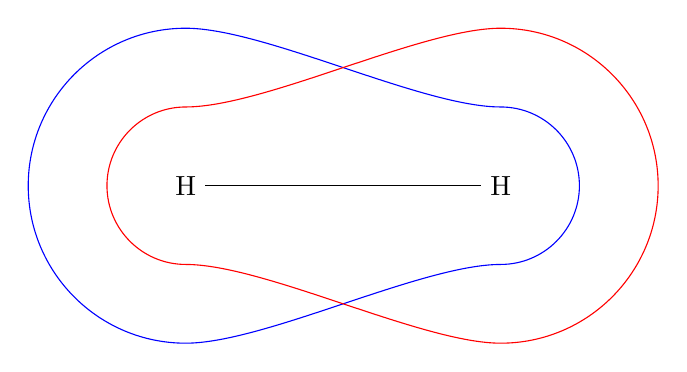
\begin{tikzpicture}
	\draw (-2,0) node[fill=white]{H} -- (2,0) node[fill=white]{H};
	\draw (-2,2)[blue] arc(90:270:2)
	.. controls +(1,0) and +(-1,0) .. (2,-1)
	arc(-90:90:1)
	.. controls +(-1,0) and +(1,0) .. (-2,2);

	\draw (-2,1)[red] arc(90:270:1)
	.. controls +(1,0) and +(-1,0) .. (2,-2)
	arc(-90:90:2)
	.. controls +(-1,0) and +(1,0) .. (-2,1);
\end{tikzpicture}

Representation of Hydrogen Gas with \\Two Single Electron Ground States Shown.
\end{center}
A common example of the exchange interaction is the ground state of hydrogen gas\footnote{Sometimes called "hydrogenic atoms" since,
despite commonly being a gas,
we don't have to assume so for the quantum analysis.}.
For reasons outside the scope of this example,
the ground states for hydrogen gas with a single electron are known to be spanned by two wave functions,
both independent of spin,
where the electron favours one atom more than another but are otherwise similar.
To analyse the ground state for hydrogen gas with two electrons it makes sense to consider combinations of these wave functions:
\[\ket{1,1},\,\ket{1,2},\,\ket{2,1},\,\ket{2,2}\]
Where $\ket{1,2}$ is the wave function where the first electron is closer to the first atom and the second electron is closer the second atom and likewise for other states.
The combination of these states with minimal energy is given by:
\[\frac{1}{\sqrt{2}}(\ket{2,1}+\ket{1,2})\]
A symmetric function.
If we similarly let $\ket{\uparrow,\downarrow}$ be the spin state were the first electron is up and the second is down we can write all our spin options for two electrons as:
\[\left.\begin{matrix}\ket{\uparrow,\uparrow}\\\frac{1}{\sqrt{2}}(\ket{\uparrow,\downarrow}+\ket{\downarrow,\uparrow})\\\ket{\downarrow,\downarrow}\end{matrix}\right\}\text{Symmetric}\quad\quad\frac{1}{\sqrt{2}}(\ket{\uparrow,\downarrow}-\ket{\downarrow,\uparrow})\bigg\}\text{Antisymmetric}\]
Noticing that there's only one antisymmetric spin option to get an antisymmetric total wave function from our symmetric spinless wave function our only choice is:
\[\frac{1}{2}(\ket{\uparrow,\downarrow}-\ket{\downarrow,\uparrow})(\ket{2,1}+\ket{1,2})\]
Hence despite the ground state seemingly not putting any requirements on spin a requirements arises from the spin statistics of indistinguishable particles which does.
\\

Two quick interesting notes to include here are:
\begin{enumerate}
\item Anyone that enjoyed high-school chemistry should be please to see that we have recovered the idea of a covalent bond between the two hydrogen.
As the ground state of two first group elements being two electrons of in opposite spin being shared between them.
\item I'm being somewhat lose when saying "spinless wave function". 
What I technically mean is that if our total wave function belongs to the vector space $V$ and our available spins form the space $S$ then our spinless wave function is from a space $W$ such that $V=S\otimes W$.
This works because our space of wave functions happen to be independent of spin meaning we can factorize $V$ into such a form.
This also means that the multiplication in our final expression is actually the tensor product.
\end{enumerate}

%% A Draft for the Exchange Interaction that I ended up not liking enough to continue with, but also didn't want to delete.
% 
% \subsection{Exchange Interaction Draft}
% Let $\ket{\Phi_1}$ and $\ket{\Phi_2}$ be wave functions for indistinguishable particles that include spin.
% We express these states in the position-spin base in the standard way:
% \[\ket{\Phi_n} = \int\Phi_n(r_n)\ket{s_n,r_n}\,dr_n\]
% Observe that theres no summation over $s_n$ since it is fixed for each $\ket{\Phi_n}$.
% It could be included anyway and just zero half the coefficients,
% but I find that too messy.
% \\
% 
% Construct basis for the combined systems through the standard:
% \[\ket{s_1,s_2,r_1,r_2} = \ket{s_1,r_1}\otimes\ket{s_2,r_2}\]
% We can get some immediate results from just by analysing the basis, let:
% \begin{equation*}
% \begin{aligned}
% \hat{P}_s\ket{s_1,s_2,r_1,r_2} =& k_s\hat{P}_s\ket{s_2,s_1,r_1,r_2}\\ 
% \hat{P}_r\ket{s_1,s_2,r_1,r_2} =& k_r\hat{P}_s\ket{s_1,s_2,r_2,r_1}\\ 
% \hat{P}\ket{s_1,s_2,r_1,r_2} =& k\hat{P}_s\ket{s_1,s_1,r_2,r_1}\\ 
% \end{aligned}
% \end{equation*}
% The last operator is swapping the two indistinguishable particles and hence is governed by standard exchange symmetry, meaning $k=1$ for bosons and $k=-1$ for fermions. 
% 
% The other operators swap just position and spin and are governed by similar rules.
% To see why observe that the left and right states have the same observables,
% hence the operators are unitary,
% but the operators are also involuntary:
% \[\hat{P}_s^2 = \hat{P}_r^2 = I\]
% This means:
% \[\ket{s_1,s_2,r_1,r_2} = \hat{P}_s^2\ket{s_1,s_2,r_1,r_2}=k_s^2\ket{s_1,s_2,r_1,r_2}\]
% Requiring $k_s = \pm 1$,
% and likewise for $k_r$.
% 
% Let $\hat{H}_1$ and $\hat{H}_2$ be operators for the respective states.
% Define a new operator:
% \[\hat{H} = \hat{H}_1\otimes I + I\otimes\hat{H}_2+\hat{H}_{12}\]
% Where $\hat{H}_{12}$ is the "interaction" term.
% 
% \subsection{Future Plans}
% Clebsch–Gordan coefficients and triplet states
% \[\bra{\Phi_\pm}H\ket{\Phi_\pm} = \frac{1}{2}\bigg(\bra{\Phi_+}H\ket{\Phi_+}+\bra{\Phi_-}H\ket{\Phi_-}\bigg)\pm\frac{1}{2}\bigg(\bra{\Phi_+}H\ket{\Phi_+}-\bra{\Phi_-}H\ket{\Phi_-}\bigg)\]
% Non-separable, no classic interpretation.
% Magnetite and lodestone
% Open problem, clearly not from another magnetic but from an current induced field.
% Not made from another magnet Earths magnetic field is likely too weak, maybe lightning bolt
%\begin{center}
%\begin{tikzpicture}
%	% E_0 Levels
%	\draw [red] (1,2) node[left] {$E_0$}--(3,2);
%	\draw [red] (4,3)--(6,3) node [midway] {$\big\uparrow\big\uparrow$};
%	\draw [red] (4,1)--(6,1) node [midway] {$\big\uparrow\big\downarrow$};
%	\draw [red] (7,3)--(9,3) node [midway] {$\big\downarrow\big\downarrow$};
%	\draw [red] (7,1)--(9,1) node [midway] {$\big\downarrow\big\uparrow$};
%
%	% E_0 links
%	\draw [blue, dashed] (3,2) -- (4,3);
%	\draw [blue, dashed] (3,2) -- (4,1);
%	\draw [blue, dashed] (6,3) -- (7,3);
%	\draw [blue, dashed] (6,1) -- (7,1);
%
%	% E_1 Levels
%	\draw [red] (1,7) node[left] {$E_1$}--(3,7);
%	\draw [red] (4,8)--(6,8) node [midway] {$\big\uparrow\big\uparrow$};
%	\draw [red] (4,6)--(6,6) node [midway] {$\big\uparrow\big\downarrow$};
%	\draw [red] (7,8)--(9,8) node [midway] {$\big\downarrow\big\downarrow$};
%	\draw [red] (7,6)--(9,6) node [midway] {$\big\downarrow\big\uparrow$};
%
%	% E_1 links
%	\draw [blue, dashed] (3,7) -- (4,8);
%	\draw [blue, dashed] (3,7) -- (4,6);
%	\draw [blue, dashed] (6,8) -- (7,8);
%	\draw [blue, dashed] (6,6) -- (7,6);
%\end{tikzpicture}
%
%Naïve Energy Level Diagram
%\end{center}
%\[\left.\begin{matrix}\ket{1,1}\\\frac{1}{\sqrt{2}}(\ket{1,2}+\ket{2,1})\\\ket{2,2}\end{matrix}\right\}\text{Symmetric}\quad\quad\frac{1}{\sqrt{2}}(\ket{1,2}-\ket{2,1})\bigg\}\text{Antisymmetric}\]

% Copyright 2024 Kieran W Harvie. All rights reserved.

\section{Clebsch–Gordan Coefficients}
Moving from classical mechanics where a system with two subsystems $V_1$ and $V_2$ is identified with $V_1\oplus V_2$ to quantum mechanic where it's instead identified with $V_1\otimes V_2$ brings many interesting changes.
A notable change is how angular momentum begins to add in a counterintuitive way which lead to a lot of systemizations:
"It's a vector!", "No it's a rotating cone!", "No the cones have to be set up a certain way!".
Well I'm going to do some revision and work my way back up to the Clebsch–Gordan coefficients.
\\

Let $\hat{j}$ be the angular momentum operator and $\hat{j}_z$ the operator for the projection of angular momentum on the $z$-axis, and like wise for $\hat{j}_x$ and $\hat{j}_y$.
Physically these that these operators satisfy the following commuting relations:
\[[\hat{j}_x,\hat{j}_y]=i\hbar\hat{j}_z,\quad
[\hat{j}_y,\hat{j}_z]=i\hbar\hat{j}_x,\quad
[\hat{j}_z,\hat{j}_x]=i\hbar\hat{j}_y\]
Which can be shorten to:
\[[\hat{j}_k,\hat{j}_l]=i\hbar\varepsilon_{klm}\hat{j}_m\]
Where $\varepsilon_{jkm}$ is the standard Levi-Civita symbol where we identify $x$ with $1$, $y$ with $2$, $z$ with $3$.
\\

The first problem with the transition is already clear,
these operators don't commute!
To work around this problem we instead consider the operator $\hat{j}^2$
\[\hat{j}^2 = \hat{j}_x^2+\hat{j}_y^2+\hat{j}_z^2\]
This operator does commute with the projection onto the axis:
\begin{equation*}
\begin{aligned}
	[\hat{j}^2,\hat{j}_z] =& (\hat{j}_x^2j_z-j_z\hat{j}_x^2)+(\hat{j}_y^2\hat{j}_z-\hat{j}_z\hat{j}_y^2)+(\hat{j}_z^2\hat{j}_z-\hat{j}_z\hat{j}_z^2) \\
	=& \hat{j}_x[\hat{j}_x,j_z]+[\hat{j}_x,j_z]\hat{j}_x+\hat{j}_y[\hat{j}_y,\hat{j}_z]+[\hat{j}_y,\hat{j}_z]\hat{j}_y \\
	=& i\hbar(-\hat{j}_x\hat{j}_y-\hat{j}_y\hat{j}_x+\hat{j}_y\hat{j}_x+\hat{j}_x\hat{j}_y) \\
	=& \hat{0}\\
\end{aligned}
\end{equation*}
This means we can find a common eigenbasis of $\hat{j}_z$ and $\hat{j}^2$\footnote{
	And likewise for $\hat{j}_x$ and $\hat{j}_y$ (but only one at a time) however $z$ is the conventional axis.
	Also I can't shake the feeling that I'm missing some point when getting a common eigenbasis from commuting hermitian operators.}.
We label these states $\ket{j,m}$ and,
for application reasons,
the relationship between the eigenvalues and labels aren't as expected.
Instead of using the eigenvalue as the label they are related by:
\begin{equation*}
\begin{aligned}
	\hat{j}^2\ket{j,m} =& \hbar^2 j(j+1)\ket{j,m},\quad j\in\left\{0,\frac{1}{2},1,\frac{3}{2},\cdots\right\}&\\
	\hat{j}_z\ket{j,m} =& \hbar m\ket{j,m}\,\quad m\in\left\{-j,-j+1,\cdots,j-1,j\right\}&\\
\end{aligned}
\end{equation*}

Note that an immediate result from $\hat{j}$ and $\hat{j}_k$ being hermitian is that their eigenvalues are real,
meaning we only have to assume $m\in\mathbb{Z}$ since:
\[\begin{aligned}
	j(j+1) =& \frac{1}{\hbar^2}\bra{j,m}\hat{j}^2\ket{j,m}\\
	=&\frac{1}{\hbar^2}\bra{j,m}\hat{j}^2_x\ket{j,m}+\frac{1}{\hbar^2}\bra{j,m}\hat{j}^2_y\ket{j,m}+\frac{1}{\hbar^2}\bra{j,m}\hat{j}^2_z\ket{j,m}\\
	\geq& \frac{1}{\hbar^2}\bra{j,m}\hat{j}_z^2\ket{j,m}\\
	=& m^2
\end{aligned}\]

\subsection{Total Angular Momentum}
The total angular momentum $\hat{J}$ on $V_1\otimes V_2$ is defined as expected:
\[\hat{J} = \hat{j_1}\otimes\hat{I}_2+\hat{I}_1\otimes\hat{j_2}\]
Observe that the left element of the tensor product always has to be from $V_1$ and carries a $1$ subscript,
and like wise for right and $2$.
This is annoying (even the identity elements need them),
so will be omitted.
Since we will be in the same tensor product space remember which space each element has to be from an mentally append the subscript.
\\

In this convention the total angular momentum operator would be written as:
\[\hat{J} = \hat{j}\otimes\hat{I}+\hat{I}\otimes\hat{j}\]
And the projection onto the $k$th axis as
\[\hat{J}_k = \hat{j}_k\otimes\hat{I}+\hat{I}\otimes\hat{j}_k\]

\subsubsection{Commutator Identities}
We will use the following two commutator identities:
\[[A\otimes B\,,\,C\otimes D] = (AC)\otimes(BD)-(BD)\otimes(AC)\]
\[[A+B,C+D] = [A,C]+[A,D]+[B,C]+[B,D]\]
And the following two sub cases of the first:
\[[A\otimes \hat{I}\,,\,C\otimes \hat{I}] = [A,C]\otimes\hat{I}\]
\[[A\otimes \hat{I}\,,\,\hat{I}\otimes D] =\hat{0}\]
While these identities can be directly algebraically verified they are worth clearly saying up front.

\subsubsection{Commuting Problems}
Unfortunately $\hat{J_k}$ follows the same commuting identities of $\hat{j_k}$,
preventing common eigenstates:
\begin{equation*}
\begin{aligned}
	[\hat{J}_k\,,\,\hat{J}_l] =& [\hat{j}_k\otimes\hat{I}+\hat{I}\otimes\hat{j}_k\,,\,\hat{j}_l\otimes\hat{I}+\hat{I}\otimes\hat{j}_l] \\
	=&[\hat{j}_k\otimes\hat{I}\,,\,\hat{j}_l\otimes\hat{I}]+[\hat{j}_k\otimes\hat{I}\,,\,\hat{I}\otimes\hat{j}_l] \\
	&+[\hat{I}\otimes\hat{j}_k\,,\,\hat{j}_l\otimes\hat{I}]+[\hat{I}\otimes\hat{j}_k\,,\,\hat{I}\otimes\hat{j}_l] \\
	=& [\hat{j}_k\,,\,\hat{j}_l]\otimes \hat{I}+\hat{I}\otimes[\hat{j}_k\,,\,\hat{j}_l]\\
	=& i\hbar\varepsilon_{klm}(\hat{j}_m\otimes\hat{I}+\hat{I}\otimes\hat{j}_m)\\
	=& i\hbar\varepsilon_{klm}\hat{J}_m\\
\end{aligned}
\end{equation*}
But this isn't such a big deal,
since we also have:
\[[\hat{J}^2,\hat{J}_z]=\hat{0}\]
However the use of $\hat{J}^2$ comes with its own problem in an awkward cross term: 
\[\hat{J}^2 = \hat{j}^2\otimes\hat{I}+\hat{I}\otimes\hat{j}^2+2\hat{j}\otimes\hat{j}\]

\subsubsection{Bases}
These results give us two bases for $V_1\otimes V_2$.
First is the natural basis from its definition as a tensor product:
\[\ket{m_1,j_1}\otimes\ket{m_2,j_2} = \ket{m_1,m_2,j_1,j_2}\]
With the natural interpretation of the subsystem $V_1$ being $\ket{m_1,j_1}$ and $V_2$ being in $\ket{m_2,j_2}$.
Second is the common eigenbasis of the commuting hermitian operators $\hat{J}^2$ and $\hat{J}_z$ defined by:
\begin{equation*}
\begin{aligned}
	\hat{J}^2\ket{J,M} =& \hbar^2 J(J+1)\ket{J,M}\\
	\hat{J}_z\ket{J,M} =& \hbar M\ket{J,M}\\
\end{aligned}
\end{equation*}
With the natural interpretation of the angular momentum and projected angular momentum of the supersystem.
We can convert between the two,
i.e. given the total angular momentum calculate the superposition subsystems or vise-versa,
is done in the normal way:
\[\ket{J,M} = \sum_{m_1,m_2,j_1,j_2}\ket{m_1,m_2,j_1,j_2}\braket{m_1,m_2,j_1,j_2}{J,M}\]
Note that despite the bounds being absent the use of a sum is justified by $\ket{m_1,m_2,j_1,j_2}$ being a base,
hence any state is in the span.
\\

But there's still a lot of them can we know in advance in any are $0$?
Well consider the following manipulation:
\[\begin{aligned}
	&\sum_{m_1,m_2,j_1,j_2}\hbar(m_1+m_2)\ket{m_1,m_2,j_1,j_2}\braket{m_1,m_2,j_1,j_2}{J,M}\\
	=&\sum_{m_1,m_2,j_1,j_2}(\hat{j}_z\otimes\hat{I}+\hat{I}\otimes\hat{j}_z)\ket{m_1,m_2,j_1,j_2}\braket{m_1,m_2,j_1,j_2}{J,M}\\
	=&\sum_{m_1,m_2,j_1,j_2}\hat{J}_z\ket{m_1,m_2,j_1,j_2}\braket{m_1,m_2,j_1,j_2}{J,M}\\
	=&\hat{J}_z\sum_{m_1,m_2,j_1,j_2}\ket{m_1,m_2,j_1,j_2}\braket{m_1,m_2,j_1,j_2}{J,M}\\
	=&\hat{J}_z\ket{J,M}\\
	=&\hbar M\ket{J,M}\\
	=&\hbar M\sum_{m_1,m_2,j_1,j_2}\ket{m_1,m_2,j_1,j_2}\braket{m_1,m_2,j_1,j_2}{J,M}\\
\end{aligned}\]
Taking the first expression away from the final gives:
\[
	0=\sum_{m_1,m_2,j_1,j_2}\hbar(M-(m_1+m_2))\ket{m_1,m_2,j_1,j_2}\braket{m_1,m_2,j_1,j_2}{J,M}\\
\]
Hence the coefficients must be $0$ unless $M=m_1+m_2$.

\subsection{Clebsch–Gordan Coefficients}
Consider the case where we fix $j_1$ and $j_2$ of the subsystems along side the $J$ and $M$ of the supersystem.
This is a common application when the subsystems are elementary particles with fixed $j_1$ and $j_2$ and the supersystem is in a state with fixed $J$ and $M$ due to externalities. 
Instead of considering the whole of $V_1\otimes V_2$ instead just consider the subspace:
\[\spn\{\ket{m_1,j_1}\mid\{|m_1|\leq j_1\}\}\otimes\spn\{\ket{m_2,j_2}\mid\{|m_2|\leq j_2\}\}\]
After proving closure everything we proved about $V_1\otimes V_2$ applies here,
prefixing $[j_1,j_2]$ to the kets to denote the subspace,
or dropping when the meaning is clear.
We can use these results to express the supersystem as a superposition of different $m_1$ and $m_2$.
\[\ket{[j_1,j_2],J,M} = \sum_{k=-j_1}^{j_1}\ket{k,M-k,j_1,j_2}\braket{k,M-k,j_1,j_2}{[j_1,j_2]J,M}\]
(Note, alternative parametrizations of this sum are common and available)
These coefficients $\braket{m_1,m_2,j_1,j_2}{J,M}$ are the Clebsch–Gordan coefficients and can be looked up in readily available and iconically shaped tables.

\subsection{Rotating Cones}
In the beginning I talked about interpreting quantum angular momentum as rotating cones,
what did I mean by this?
Well consider the set of points in $\mathbb{R}^3$ with a known distance to the origin and known $Z$ component.
We get a circle centered on the $Z$ axis at that known hight.
The analogy to quantum angular momentum is obvious:
\begin{center}
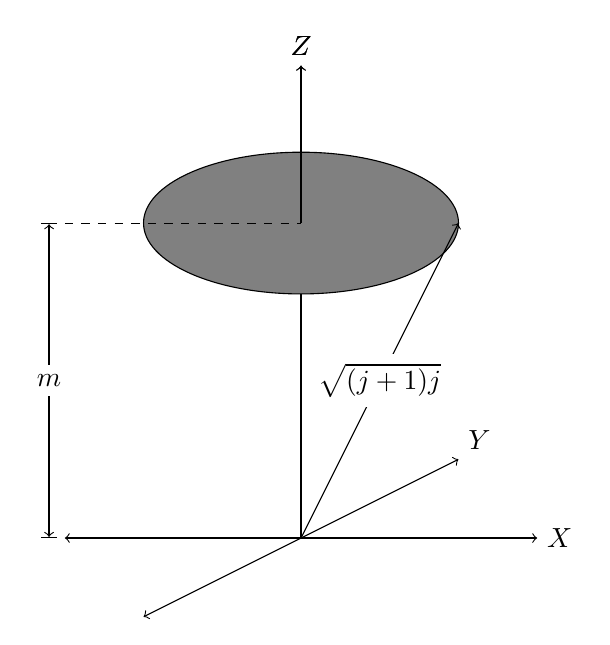
\begin{tikzpicture}
	\draw[<->] (-3,0)--(3,0) node[right]{$X$};
	\draw[->] (0,0)--(0,6) node[above]{$Z$};
	\draw[<->] (-2,-1)--(2,1) node[above right]{$Y$};
	\draw[fill = gray] (0,4) circle[x radius = 2, y radius = 0.9];
	\draw[->] (0,4)--(0,6) node[above]{$Z$};

	\draw[dashed] (-3,4)--(0,4);
	\draw[|<->|] (-3.2,0)--  (-3.2,4) node[midway,fill=white]{$m$};

	\draw[->] (0,0)--(2,4) node[midway,fill=white]{$\sqrt{(j+1)j}$} ;
\end{tikzpicture}
\end{center}
But how do we add momentum this way?
Well if we consider the most simple case of adding a one of these disks to to itself.
We simply take one point on the edge of the disk and scale up accordingly:
\begin{center}
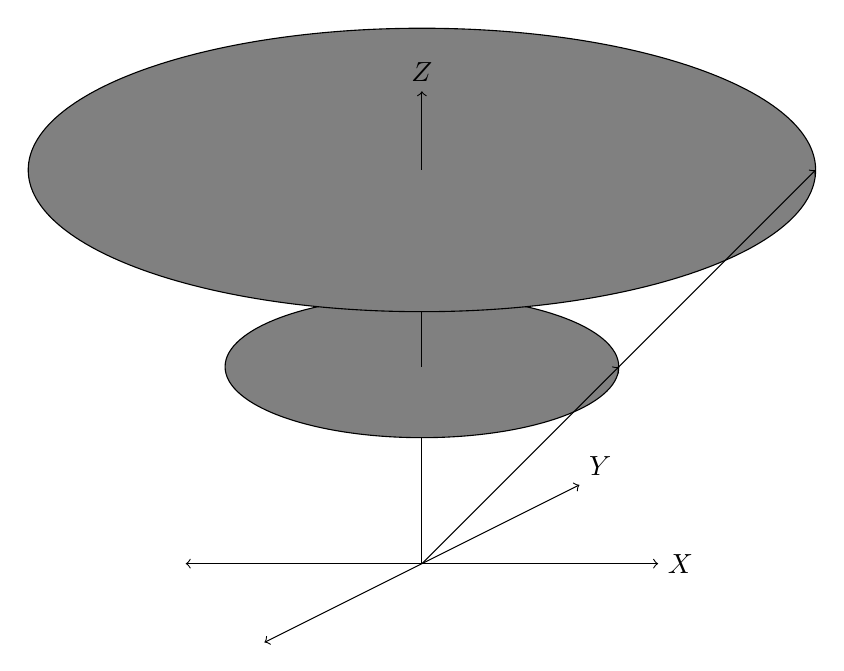
\begin{tikzpicture}
	\draw[<->] (-3,0)--(3,0) node[right]{$X$};
	\draw[<->] (-2,-1)--(2,1) node[above right]{$Y$};
	\draw (0,0)--(0,2.5);
	\draw[fill = gray] (0,2.5) circle[x radius = 2.5, y radius = 0.9];
	\draw (0,2.5)--(0,5);
	\draw[fill = gray] (0,5) circle[x radius = 5, y radius = 1.8];
	\draw[->] (0,5)--(0,6) node[above]{$Z$};

	\draw[->] (0,0)--(2.5,2.5);
	\draw[->] (2.5,2.5)--(5,5);
\end{tikzpicture}
\end{center}
This corresponds to the following equation:
\[\ket{\left[\frac{1}{2},\frac{1}{2}\right],1,1}=\frac{1}{\sqrt{2}}\left(\ket{\frac{1}{2},\frac{1}{2}}+\ket{\frac{1}{2},\frac{1}{2}}\right)\]
But this idea isn't complete because we need to incorporate relative phase of the basis vectors into the picture.
For example we have could be in phase:
\begin{center}
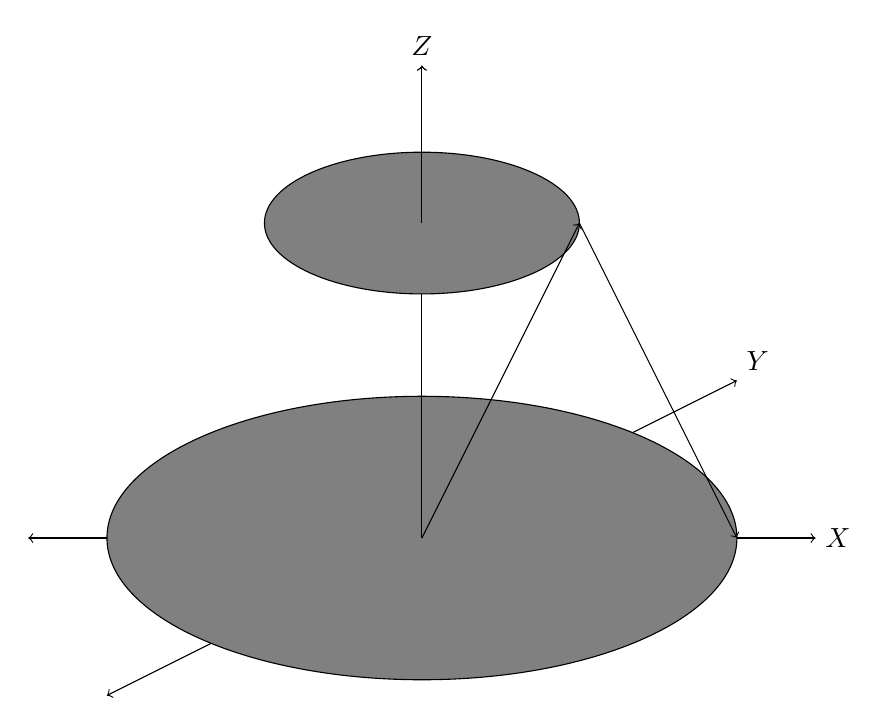
\begin{tikzpicture}
	\draw[<->] (-5,0)--(5,0) node[right]{$X$};
	\draw[<->] (-4,-2)--(4,2) node[above right]{$Y$};
	\draw[fill = gray] (0,0) circle[x radius = 4, y radius = 1.8];
	\draw[->] (0,0)--(0,6);
	\draw[fill = gray] (0,4) circle[x radius = 2, y radius = 0.9];
	\draw[->] (0,4)--(0,6) node[above]{$Z$};

	\draw[->] (0,0)--(2,4);
	\draw[->] (2,4)--(4,0);
\end{tikzpicture}
\end{center}
\[\ket{1,0}=\frac{1}{\sqrt{2}}\left(\ket{\frac{1}{2},-\frac{1}{2}}+\ket{-\frac{1}{2},\frac{1}{2}}\right)\]
As well as in opposite phase:
\begin{center}
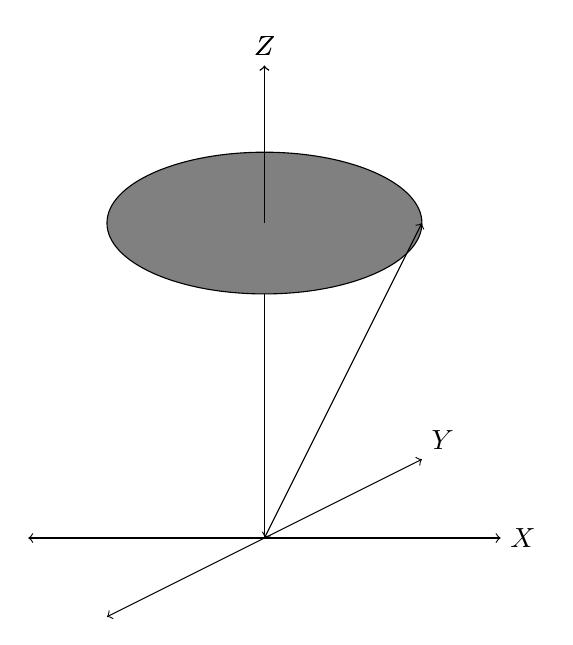
\begin{tikzpicture}
	\draw[<->] (-3,0)--(3,0) node[right]{$X$};
	\draw[->] (0,0)--(0,6) node[above]{$Z$};
	\draw[<->] (-2,-1)--(2,1) node[above right]{$Y$};
	\draw[fill = gray] (0,4) circle[x radius = 2, y radius = 0.9];
	\draw[->] (0,4)--(0,6) node[above]{$Z$};

	\draw[<->] (0,0)--(2,4);
\end{tikzpicture}
\end{center}
\[\ket{0,0}=\frac{1}{\sqrt{2}}\left(\ket{\frac{1}{2},-\frac{1}{2}}-\ket{-\frac{1}{2},\frac{1}{2}}\right)\]
As suggested by the picture the relative phase of the basis vectors is the relative phase of the $\mathbb{R}^3$ vectors as they rotate around.
In the first example the two basis vectors are in phase so both vectors start at $0$ degrees and rotate together.
While in the second example the two basis vectors are in opposite phase so one starts at $0$ degrees and the other at $180$ meaning as they rotate they cancel out.
\\

This is what's meant by "Rotating cones set up a certain way".
First you convert vectors into cones using the initial geometry analogy.
Then you scale them by the basis vectors' coefficients relative magnitude and rotate them by their relative phase.
Finally you rotate the vectors at the same angular velocity and see which disk is traced out.
\\

(Note the reason they are disks instead of cones is because it's surprisingly difficult to draw cones in tikz.
The reader is invited to use their imagination to fill in the missing sides.)

\subsection{Conclusion}
The previous section concludes the revision I needed and I'm getting kind of tired of thinking about Clebsch–Gordan theory.
However the topic is rich and I can see myself coming back later and appending to this section,
bellow is a wish-list of explorations on my return:
\begin{itemize}
	\item Actually calculating some Clebsch–Gordan coefficients.
		I normally just look them up confident someone has done them correctly.
	\item Talk about the total angular momentum raising and lowering operators:
		\[\hat{J}_\pm = \hat{j}_\pm\otimes I + I\otimes\hat{j}_\pm\]
	\item Talk about Lie Algebras.
		Both how they apply to the communicator section in general and how the calculations used here are the basis of a representation of the SU(2) Lie Algebra.
	\item There relationship between the coefficients and spherical harmonics.
\end{itemize}

% Copyright 2024 Kieran W Harvie. All rights reserved.

\section{Quadratic Form Hadamard Matrix}
Consider the following equality between quadratic forms:
\[\begin{aligned}
	&w_{+,+}(x+y+z)^2+w_{+,-}(x+y-z)^2+w_{-,+}(x-y+z)^2+w_{-,-}(x-y-z)^2\\
	=&h_0(x^2+y^2+z^2)+2h_{xy}xy+2h_{xz}xz+2h_{yz}yz\\
\end{aligned}\]
Their coefficients are related by:
\[
	\begin{bmatrix}1&1&1&1\\1&-1&1&-1\\1&1&-1&-1\\1&-1&-1&1\\\end{bmatrix}
	\begin{bmatrix}w_{+,+}\\w_{+,-}\\w_{-,+}\\w_{-,-}\end{bmatrix}
	=\begin{bmatrix}h_0\\h_{xz}\\h_{xy}\\h_{yz}\end{bmatrix}
\]
This might already be a cool result as expressions with squares like this are often useful.
But the matrix is $H_4$, the fourth order Hadamard Matrix,
a known matrix with many cool properties like:
\[H_n^2=4I_4\]

\subsection{Sedrakyan's Inequality}
If we express a general linear relation between $x$,$y$, and $z$ as:
\[\begin{aligned}
	&a_0x+a_1y+a_2z\\
	=& t(x+y+z) + (\mu_{+,-}-t)(x+y-z)\\
	&+(\mu_{-,+}-t)(x-y+z)+(\mu_{-,-}-t)(x-y-z)\\
	=& |\mu_{+,+}-t|\sgn(\mu_{+,+}-t)(x+y+z) + |\mu_{+,-}-t|\sgn(\mu_{+,-}-t)(x+y-z)\\
	&+|\mu_{-,+}-t|\sgn(\mu_{-,+}-t)(x-y+z)+|\mu_{-,-}-t|\sgn(\mu_{-,-}-t)(x-y-z)\\
\end{aligned}\]
Where:
\[\mu_{+,+} =0,\,\mu_{+,-} = \frac{a_0+a_1}{2},\,\mu_{-,+}=\frac{a_0+a_2}{2},\,\mu_{-,-}=\frac{a_1+a_2}{2}\]
Assuming $t$ is not equal to any of the $\mu_S$, we can apply Sedrakyan's Inequality to give: 
\[\begin{aligned}
	&\frac{(a_0x+a_1y+a_2z)^2}{|t|+|\mu_{+,-}-t|+|\mu_{-,+}-t|+|\mu_{-,-}-t|}\\
	\leq&\frac{(x+y+z)^2}{|t|}+\frac{(x+y-z)^2}{|\mu_{+,-}-t|}+\frac{(x-y+z)^2}{|\mu_{-,+}-t|}+\frac{(x-y-z)^2}{|\mu_{-,-}-t|}
\end{aligned}\]
When $t$ is equal to one or more of the $\mu_S$ simply use a lower dimensional Sedrakyan's Inequality for a similar result.
Combining these gives:
\[\begin{aligned}
	&(a_0x+a_1y+a_2z)^2\\
	\leq&w_{+,+}(x+y+z)^2+w_{+,-}(x+y-z)^2+w_{-,+}(x-y+z)^2+w_{-,-}(x-y-z)^2\\
\end{aligned}\]
With:
\[w_S = \begin{cases}|\mu_S-t|^{-1}(|t|+|\mu_{+,-}-t|+|\mu_{-,+}-t|+|\mu_{-,-}-t|)&t\neq \mu_S\\0&t=\mu_S\end{cases}\]
(Note that the orginal LHS denominator being $0$ isn't an issue when at lest one $a_k$ is nonzero).
\\

Meaning we can use the main result to express a bound of $(a_0x+a_1y+a_2z)^2$ as a linear sum of $x^2+y^2+z^2$, $xy$, $xz$, and $yz$.

% Copyright 2024 Kieran W Harvie. All rights reserved.

\section{Incidence Algebra}
While working on the harmonic series I got an itch to revise some incidence algebra.
This is because of the use of the inclusion-exclusion principle,
which is beautifully generalized by the structure. 

\subsection{Poset Revision}
A poset $P$ is set with an operator $\preceq$ referred to as the `partial order' and works as one would expect, meaning for $x,y,z\in P$ :
\begin{itemize}
	\item {\bf Reflexivity:}  $x\preceq x$.
	\item {\bf Antisymmetry:}  If $x\preceq y$ and $y\preceq x$ then $x=y$.
	\item {\bf Transitivity:}  If $x\preceq y$ and $y\preceq z$ then $x\preceq z$.
\end{itemize}
We write $x\prec y$ is $x\preceq$ and $x\neq y$ and a chain is a subset of $P$ such that:
\[x_0\prec x_1 \prec x_2 \prec \dots \prec x_n\]
A multichain is a subset of $P$ such that:
\[x_0\preceq x_1 \preceq x_2 \preceq \dots \preceq x_n\]
A closed interval $[x,y]$ is a subset of $P$ defined as:
\[[x,y] = \{z\,:\,x\preceq z\preceq y \text{ where }x,y,z\in P\}\]
The set of all intervals of a $P$ is denoted $\operatorname{Int}(P)$ and a locally finite poset $P$ is one where each closed interval is finite.

\subsection{Incidence Algebra Definition}
The Incidence Algebra of $P$ over $K$ is denoted $I(P,K)$ where the vector space is the space of functions $K^{\operatorname{Int}(P)}$ with addition and scalar multiplication defined in the normal way.
The bilinear function of the algebra is called convolution and is defined as:
\[(f*g)([x,y]) = \sum_{z\in [x,y]}f([x,z])g([z,y])\]
Where meaning is obvious a lot of symbols are dropped:
\[fg[x,y] = \sum_{z\in [x,y]}f[x,z]g[z,y]\]
Some special names elements are the delta and zeta functions:
\[\zeta[x,y] = 1,\quad\delta[x,y] = \begin{cases}1&x=y\\0&x\neq y\end{cases}\]
These functions are defined their useful convolution properties:
\begin{equation*}
\begin{aligned}
	f\zeta[x,y] =& \sum_{z\in [x,y]}f[x,z]\\
	\zeta f[x,y] =& \sum_{z\in [x,y]}f[z,y]\\
	f\delta[x,y] =& \delta f[x,y] = f[x,y]\\
\end{aligned}
\end{equation*}
We can see that the set of invertible functions $K^{\operatorname{Int}(P)}$ are a group with unit element $\delta$.
To this end  with define a new function $\mu$ called the Möbius function:
\[\mu[x,y] = \begin{cases}1&x=y\\-\sum_{x\preceq z\prec y}\mu(x,z)&x\prec y\\0&y\prec x\\\end{cases}\]
You can show that:
\[\mu\zeta = \delta\]
An important use for this group is as a group action from this group onto $K^P$ such that:
\[(f\cdot a)(x) = \sum_{y\preceq x}f(y)a[y,x]\]

\subsection{General Inclusion-Exclusion Principle}
Assume all the previous results are true\footnote{Prove them yourself.} we get the following corollary.
Let $f,g\in K^P$ then:
\[g(x) = (f\cdot \zeta)(x) \Leftrightarrow f(x) = (g\cdot \mu)(x)\]
Or more verbosely:
\[g(x) = \sum_{y\preceq x}f(y) \Leftrightarrow f(x) = \sum_{y\preceq x}g(y)\mu[y,x]\]
For a sketch of how this is generalization of the more common inclusion-exclusion principle consider the following:
\begin{enumerate}
	\item Let $(A_i)_{i\in I}$ be a family of sets indexed by $I$ and let $P$ be the poset of subsets of $I$ ordered by inclusion.
	This makes $\mu[S,T] = (-1)^{T/S}$
	\item Define $f:P\rightarrow \mathbb{N}$ where $f(T)$ is the number of elements $a$ such that:
		\[\left\{a \in \bigcup_{i\in I/T}A_i \mid i\in T \Rightarrow a\not\in A_i \right\}\]
	In natural language, this is set elements in the sets indexed by $I/T$ but not in the sets indexed by $T$.
	\item These sets are mutually exclusive so we directly get:
		\[g(T)=\begin{cases}\left|\bigcap_{i\in I/T}A_i\right| T\neq I\\\left|\bigcup_{i\in I\phantom{/I}}A_i\right|T=I\end{cases}\]
	\item $f(I)=0$ because $\bigcup_{i\in I/I}A_i = \varnothing$ applying the general inclusion-exclusion principle to $f(I)$ we get: 
		\[0=\left|\bigcup_{i\in I}A_i\right|+\sum_{T\subset I}\left|\bigcap_{i\in I/T}A_i\right|(-1)^{I/T}\quad\square\]
\end{enumerate}

\subsection{A Section Where I Drily Preform Calculations}
In this section I will preform some of the calculations I glossed over for the sketch of the common inclusion-exclusion principle proof,
all notation is inherited from there.

\subsubsection{Calculating $\mu[S,T]$:}
We will only consider the case $S\subset T$ and define $n=|T/S|$,
as other cases are given by the definition of $\mu$.
In this case $T/S$ contains at least on element and we can consider sets $X$ such that:
\[\varnothing\subseteq X\subset T/S\]
An important and immediate result is that $S$ and all $X$ are mutually exclusive as:
\[X\cup S \subset (T/S)\cup S = \varnothing\]
Hence sets $X$ such that $|(X\cup S)/S|=|X|=k$ are the $k$ elements subsets of $T/S$,
meaning there are $\binom{n}{k}$ of them.
\\

For the inductive assumption we assume for all sets $X$ such that:
\[|(S\cup X)/S| = k < n = |T/S|\]
We have:
\[\mu[S,S\cup X] = (-1)^{|(S\cup X)/S|} = (-1)^k\]
These are clearly the sets we just considered meaning we can reparametrize the following sum to get:
\begin{equation*}
\begin{aligned}
	\mu[S,T] =& -\sum_{S\subseteq X\subset T}\mu[S,X] \\
	=&-\sum_{\varnothing\subseteq X\subset T/S}\mu[S,S\cup X]\\
	=& -\left(\sum_{k=0}^{n-1}\binom{n}{k}(-1)^k\right)\\
	=& -\left(-(-1)^{n+1}+\sum_{k=0}^{n}\binom{n}{k}(-1)^k\right)\\
	=& -\left(-(-1)^{n+1}+(1-1)^n\right)\\
	=& (-1)^{n}\\
\end{aligned}
\end{equation*}
As required.

\subsubsection{Formalization of $f(T)$:}
To cleanly formalize $f(T)$ we will define a new utility function $\chi:\cup_{i\in I}A_i \rightarrow P$ such that:
\[\chi(a) = \{i\mid a\in A_i\}\]
In natural language $a$ is in the sets indexed by $\chi(a)$ and not in the sets indexed by $I/\chi(a)$,
hence $f(T)$ can be defined as:
\[f(T) = \left|\left\{a\in \bigcup_{i\in I}A_i \mid I/\chi(a)=T\right\}\right|\]
An important corollary of this formalization is:
\[T\neq T' \Rightarrow f(T)+f(T') =\left|\left\{a\in \bigcup_{i\in I}A_i \mid I/\chi(a)\in\{T,T'\}\right\}\right| \]
This follows from the underlying sets being mutually exclusive:
\[T\neq T' \Rightarrow \left\{a\in \bigcup_{i\in I}A_i \mid I/\chi(a)=T\right\}\cup\left\{a\in \bigcup_{i\in I}A_i \mid I/\chi(a)=T'\right\}=\varnothing\]
Mutual exclusivity doesn't come from any unique property of $\chi$ beyond being a function,
to see let $X$ be any set and $f$ be any function with domain $X$ and consider:
\[a\neq b\Rightarrow\{x\in X | f(x) = a\}\cup\{x\in X| f(x) = b\} = \varnothing\]
Assume $a=b$ but that the two sets do intersect then there would exist an element $x_0$ in that intersection such that:
\[a = f(x_0) = b\]
A contradiction, hence the sets are mutually exclusive.

\subsubsection{Alternative Formalization of $f(T)$:}
Although the previous formalization is enough to recover the more common inclusion-exclusion principle
there's a more standard and interesting way to write this set when $T\neq I$,
start by considering:
\[a\in\bigcap_{i\in I/T}A_i \Leftrightarrow I/T\cap \chi(a) = I/T \Leftrightarrow I/\chi(a)\subseteq T\] 
Since, by definition, for $a$ to be in the intersection of a set of sets it must be an element of each set.
(This is why $T\neq I$ as if the set of sets is empty then the statement becomes vacuous).
Likewise for an element not being in union of a set of sets we get:
\[a\not\in\bigcup_{i\in T}A_i \Leftrightarrow T\cap \chi(a) = \varnothing \Leftrightarrow I/\chi(a)\supseteq T\]
Since $a$ can't be an element of any of the $T$ sets, combining these results gives:
\[a\in\frac{\bigcap_{i\in I/T}A_i}{\bigcup_{i\in T\phantom{/T}} A_i}\Leftrightarrow I/\chi(a) = T\]
Hence:
\[\frac{\bigcap_{i\in I/T}A_i}{\bigcup_{i\in T\phantom{/T}} A_i}=\left\{a\in \bigcup_{i\in I}A_i \mid I/\chi(a) = T\right\}\]
Meaning when $T\neq I$ it's equivalent to the previous formalization to write:
\[f(T) = \left|\frac{\bigcap_{i\in I/T}A_i}{\bigcup_{i\in T\phantom{/T}} A_i}\right|\]

\subsubsection{Calculating $g(T)$:}
Now $g(T)$ is defined as:
\[g(T) = \sum_{S\subseteq T}f(S) = \sum_{S\subseteq T} \left|\left\{a\in \bigcup_{i\in I}A_i \mid I/\chi(a) = S\right\}\right|\]
Recall the corollary in the formalization section we have:
\[g(T)  =  \left|\left\{a\in \bigcup_{i\in I}A_i \mid I/\chi(a)\subseteq T\right\}\right|\]
Also recall from the alternative formalization section that when $T\neq I$ we have:
\[a\in\bigcap_{i\in I/T}A_i \Leftrightarrow I/\chi(a)\subseteq T\]
Hence:
\[g(T)  =  \left|\left\{\bigcap_{i\in I/T}A_i\right\}\right|\]
And when $T = I$ we have:
\[g(I)  =  \left|\left\{a\in \bigcup_{i\in I}A_i \mid I/\chi(a)\subseteq I\right\}\right|\]
Which is the whole set as for all $a$ we have:
\[I/\chi(a) \subseteq I\]
As $I$ is,
by definition,
the overarching set all other sets are an element of.
Hence:
\[g(I)  =  \left|\left\{\bigcup_{i\in I}A_i\right\}\right|\]
As required.

\subsubsection{Example Calculation of $f(I)$:}
Stated explicitly,
the general inclusion-exclusion principle applied to subsets ordered by inclusion is:
\[g(T) = \sum_{S\subseteq T}f(S) \Leftrightarrow f(T) = \sum_{S\subseteq T}g(S)(-1)^{|T/S|}\]
Note: The empty set is included in both these sums.
\\

Now let the overarching set be $I = \{0,1,2\}$ giving the indexed family of sets as $\{A_0,A_1,A_2\}$.
Calculating $f$ directly gives:
\begin{equation*}
\begin{aligned}
	f(\varnothing) =& |A_0 \cap A_1\cap A_2|\\
	f(\{0\}) =& |(A_1 \cap A_2)/A_0|\\ 
	f(\{0,1\}) =& |A_2/(A_0\cup A_1)|\\ 
	f(\{0,1,2\}) =& |\varnothing| = 0\\ 
\end{aligned}
\end{equation*}
Similarly calculating $g(T)$ directly gives:
\begin{equation*}
\begin{aligned}
	g(\varnothing) =& f(\varnothing) \\
	=& |A_0\cap A_1 \cap A_2|\\
	g(\{0\}) =& f(\varnothing) + f(\{0\})\\
	=& |A_0 \cap A_1 \cap A_2| + |(A_1\cap A_2)/A_0|\\
	=& |A_1\cap A_2|\\
	g(\{0,1\}) =& f(\varnothing) + f(\{0\})+f(\{1\})+f(\{0,1\})\\
	=& |A_0 \cap A_1\cap A_2| + |(A_1\cap A_2)/A_0|+|(A_0\cap A_2)/A_1|+|A_2/(A_0\cup A_1)|\\
	=& |A_2|\\
	g(\{0,1,2\}) =& f(\varnothing) + f(\{0\})+f(\{1\})+f(\{2\})\\
	&+f(\{0,1\})+f(\{0,2\})+f(\{1,2\})+f(\{0,1,2\})\\
	=& |A_0 \cap A_1\cap A_2| + |(A_1\cap A_2)/A_0|+|(A_0\cap A_2)/A_1|+|(A_0\cap A_2)/A_1|\\
	&+|A_2/(A_0\cup A_1)|+|A_1/(A_0\cup A_2)|+|A_0/(A_1\cup A_2)|+|\varnothing|\\
	=& |A_0\cup A_1\cup A_2|\\
\end{aligned}
\end{equation*}
Applying the general inclusion-exclusion principle gives:
\[f(\{0,1,2\}) = \sum_{S\subseteq \{0,1,2\}}g(S)(-1)^{|\{0,1,2\}/S|} \Rightarrow\,0= \sum_{S\subseteq \{0,1,2\}}g(S)(-1)^{|S|}\]
Hence:
\[g(\{0,1,2\})=g(\{0,1\})+g(\{0,2\})+g(\{1,2\})-g(\{0\})-g(\{1\})-g(\{2\})+g(\varnothing)\]
And:
\[|A_0\cup A_1\cup A_2|= |A_2|+|A_1|+|A_0|-|A_1\cap A_2|-|A_0\cap A_2|-|A_0\cap A_1|+|A_0\cap A_1\cap A_2|\]

\subsubsection{Example Calculation when $T\neq I$:}
We have a cool form of $f(T)$ when $T\neq I$,
so what does that look like in the inclusion-exclusion principle?
Well start with:
\[f(\{0,1\}) = \sum_{S\subseteq \{0,1\}}g(S)(-1)^{|\{0,1\}/S|} \Rightarrow\,\left|\frac{A_2}{A_0\cup A_1}\right|= \sum_{S\subseteq \{0,1\}}g(S)(-1)^{|S|}\]
And use the previous calculations to give:
\[\left|\frac{A_2}{A_0\cup A_1}\right| = |A_2|-|A_1\cap A_2|-|A_0\cap A_2|+|A_0\cap A_1\cap A_2|\]

%\subsection{Hasse Diagram}
%\subsection{Change summation order?}
% Expand group action?
%\subsection{Invertability}
%recurisive with $\mu$

% Copyright 2024 Kieran W Harvie. All rights reserved.

\section{Geometric $\gcd$}
Let $(X,Y)\in\mathbb{N}^2_{>0}\subset \mathbb{R}^2$, it's common knowledge that the number of points with integer coordinates on the line between $(X,Y)$ and $(0,0)$, not including $(0,0)$, is $\gcd(X,Y)$.
\\

Proof of this is usually to just draw an example and hope the reader gets it by inspection:
\begin{center}
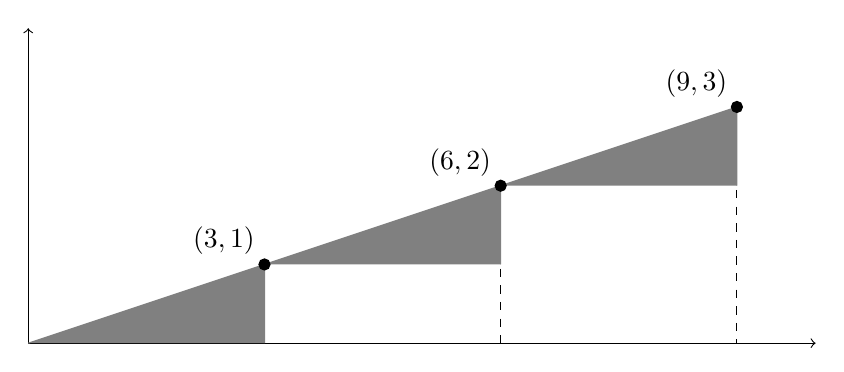
\begin{tikzpicture}[every node/.style={black}]
	\draw[->] (0,0)--(0,4);
	\draw[->] (0,0)--(10,0);

	\draw[dashed] (3,1)--(3,0);
	\draw[dashed] (6,2)--(6,0);
	\draw[dashed] (9,3)--(9,0);
	
	\filldraw[gray] (0,0)--(3,1)--(3,0);
	\filldraw[gray] (3,1)--(6,2)--(6,1);
	\filldraw[gray] (6,2)--(9,3)--(9,2);

	\filldraw (3,1) node[above left] {$(3,1)$} circle(2pt);
	\filldraw (6,2) node[above left] {$(6,2)$} circle(2pt);
	\filldraw (9,3) node[above left] {$(9,3)$} circle(2pt);
\end{tikzpicture}

Diagram for $(9,3)$ with $\gcd(9,3)=3$.
\end{center}

A sketch of a formal proof of this is the following:
\begin{enumerate}
\item There are a finite number of integer points in the square $(0,0)-(X,0)-(X,Y)-(0,Y)$,
a superset of the line between $(0,0)-(X,Y)$,
and all points of the line $(0,0)-(X,Y)$ can be uniquely ordered by their $X$ coordinate.
Hence there exits a unique integer point $(x,y)$ with minimal non-zero $X$ coordinate, this point may be $(X,Y)$ itself.
\item If a point $(x',y')$ is on the line then so is the point $(x'\mod x,y'\mod y)$.
Hence, by the minimality of $(x,y)$, all other integer points on the line are multiples of $(x,y)$ otherwise we could take $(x'\mod x,y'\mod y)$ as a smaller point.
\item Hence $x | X$, and let $d = \frac{X}{x}=\frac{Y}{y}$, then the set of integer points on the line $\{k(x,y)\,|\, k \in \{1,2,\cdots d\}\}$
\item By the minimality of $(x,y)$, $d$ must be the largest integer with the above property, meaning $d=\gcd(X,Y)$.
\end{enumerate}

But have you even considered how novel this answer is when the algebraic definition of $\gcd$ is used?
Let $(X,Y)\in\mathbb{N}^2_{>0}$ we can defined the $\gcd(X,Y)$ as:
\[\gcd(X,Y) = \min\{sX+rY\,|\,(s,r)\in\mathbb{Z}^2,\,sX+rY>0\}\]
And answer can be written as:
\begin{center}
\quad The number of solutions $(x,y)\in \mathbb{Z}^2$ to the equation $Xy-Yx=0$ such that $0<x\leq X$ is equal to $\min\{sX+rY\,|\,(s,r)\in\mathbb{Z}^2,\,sX+rY>0\}$.
\end{center}

% Copyright 2024 Kieran W Harvie. All rights reserved.

\section{Curried Function}
(This is a simple `I got something wrong and am revising' note).

There are two related but distinct operations one can apply to a multivariate function:
Currying and (partial) application.
\\

Consider the case of a bivariate\footnote{Easily generalized to higher variate functions.}
function $f:X\times Y\rightarrow Z$
(Partial) application takes the function $f$ and a value $x_0 \in X$ and outputs a new function $g:Y\rightarrow Z$ such that:
\[g(y) = f(x_0,y)\]
This operations is likely known to the reader and has the following signature:
\[\operatorname{apply}:[X\times Y\rightarrow Z]\times X\rightarrow [Y\rightarrow Z]\]
Currying a function just the function $f$ and outputs a new function $h$.
The function $h$ is itself a higher order function that takes an element $x_0\in X$ and outputs a function such that:
\[h(x_0) = g\]
This operation has the following signature:
\[\operatorname{curry}:[X\times Y\rightarrow Z]\rightarrow(X\rightarrow [Y\rightarrow Z])\]
Hence currying a function is like a middle step for partially applying it.
An important observation is that when currying a function all steps take a single parameter while partial applying needs to take two, both $x_0$ and $f$:
\[\operatorname{curry}(f)(x_0)(y) = \operatorname{apply}(f,x_0)(y)\]
This property can be useful for analysis. 
\\

Also note that currying is named after Haskell Curry.
The similarity of the term `curried function $f$' to the foods like `curried egg' and `curried sausage' is coincidental.
Won't stop me thinking of the later when people say the former.

% Copyright 2024 Kieran W Harvie. All rights reserved.

\section{Series Involving Harmonic Numbers}
I've once again wasted to much time thinking about the following series:
\[\sum_{n=1}^\infty\frac{H_n}{n^2}=2\zeta(3),\quad \sum_{n=1}^\infty\frac{H_n}{n^3}=\frac{1}{2}\zeta(2)\]
While the time wasted is a nice example of how math sometimes feels more compulsive then is healthy,
I also want to write down some theory here and hope I may avoid wasting time thinking about this in future.

\subsection{Convergence}
From the standard harmonic number bounds:
\[\ln(n)+\frac{1}{n} \leq H_n \leq \ln(n)+1\]
We can see that the series $\sum_{n=1}^\infty H_nn^{-k}$ wouldn't converge for $k=0,1$ but would for $k\geq 2$.

\subsection{Properties of $T$:}
Series of the form:
\[T(s_1,s_2;s) = \sum_{n=1}^{\infty}\sum_{m=1}^{\infty}\frac{1}{n^{s_1}m^{s_2}(n+m)^s}\]
Are called Tornheim Sums and is a case of the more general Mordell-Tornheim Sums with a depth of $2$.
The weight of a Tornheim Sum is the sum of its parameters, $s_1+s_2+s$.

\subsubsection{Argument Symmetry of $T$:}
From the symmetry of $n$ and $m$ in the bounds and summand we get:
\[T(s_1,s_2;s) = T(s_2,s_1;s)\]
By convention, we simplify Tornheim Sums by writing them with $s_1\leq s_2$.

\subsubsection{Recursion:}
Consider the following expression:
\[\frac{1}{n^{s_1}m^{s_2}(n+m)^s} = \frac{1}{n^{s_1-1}m^{s_2}(n+m)^{s+1}}+\frac{1}{n^{s_1}m^{s_2-1}(n+m)^{s+1}}\]
It can be verified pretty easily by factorizing out $n^{s_1-1}m^{s_2-1}(n+m)^s$,
double summing this expression over $n$ and $m$ we obtain:
\[T(s_1,s_2;s) = T(s_1-1,s_2;s+1)+T(s_1,s_2-1;s+1)\]
Note the weight of all terms is the same.

\subsubsection{Relation to $\zeta$ functions:}
When one or more of the arguments are zero the Tornheim Sums simplify to the (general) zeta functions:
\begin{equation*}
\begin{aligned}
	T(s_1,s_2;0) =& \sum_{n=1}^\infty\sum_{m=1}^\infty\frac{1}{n^{s_1}m^{s_2}} =\zeta(s_1)\zeta(s_2)\\
	T(0,s_2;s) =& \sum_{n=1}^\infty\sum_{m=1}^\infty\frac{1}{m^{s_2}(n+m)^s} =\zeta(s,s_2)\\
\end{aligned}
\end{equation*}

\subsubsection{Telescoping Recursion:}
Consider the last expression in more detail,
if we change how we parameterize the summation we get:
\begin{equation*}
\begin{aligned}
	T(0,s_2;s)=& \sum_{n=1}^\infty\sum_{m=1}^\infty\frac{1}{m^{s_2}(n+m)^s}\\
	=&\sum_{n=2}^\infty\frac{1}{n^s}\sum_{m=1}^{n-1}\frac{1}{m^{s_2}} \\
	=&\sum_{n=2}^\infty\frac{1}{n^s}\sum_{m=1}^n\frac{1}{m^{s_2}}-\sum_{n=2}^\infty\frac{1}{n^{s+s_2}} \\
	=&\sum_{n=1}^\infty\frac{1}{n^s}\sum_{m=1}^n\frac{1}{m^{s_2}}-\sum_{n=1}^\infty\frac{1}{n^{s+s_2}} \\
\end{aligned}
\end{equation*}
The left term is very similar to a Tornheim Sum!
All we need to do is turn the finite sum into a series.
When $s_2=1$ we can achieve this with a telescoping series,
(even though this technique is normally used to go from series to finite sum):
\begin{equation*}
\begin{aligned}
	\sum_{m=1}^{n}\frac{1}{m} =&\sum_{m=1}^\infty\left(\frac{1}{m}-\frac{1}{m+n}\right)\\
	=&n\sum_{m=1}^\infty\frac{1}{m(n+m)}\\
\end{aligned}
\end{equation*}
Substitution gives:
\begin{equation*}
\begin{aligned}
	T(0,1;s) =&\sum_{n=1}^\infty\frac{1}{n^s}\sum_{m=1}^n\frac{1}{m}-\sum_{n=1}^\infty\frac{1}{n^{s+1}} \\
	=&\sum_{n=1}^\infty\sum_{m=1}^\infty\frac{1}{n^{s-1}m(n+m)}-\sum_{n=1}^\infty\frac{1}{n^{s+1}} \\
	=&T(1,s-1;1)-T(0,s+1;0)\\
\end{aligned}
\end{equation*}
Again note that the weights are the same.

\subsection{Calculating the Original Series}
With all this machinery in place we return to the original series.
Start by writing them as Tornheim Sums by using the telescoping trick again:
\begin{equation*}
\begin{aligned}
	\sum_{n=1}^\infty\frac{H_n}{n^k} =& \sum_{n=1}^\infty\frac{1}{n^k}\left(\sum_{m=1}^{n}\frac{1}{m}\right)\\
	=& \sum_{n=1}^\infty\sum_{m=1}^\infty\frac{1}{mn^{k-1}(n+m)}\\
	=& T(1,k-1;1)\\
\end{aligned}
\end{equation*}

\subsubsection{Case $k=3$:}
This case is follows from a direct application of general recursion to $T(2,2;0)$
\[T(2,2;0) = T(1,2;1)+T(2,1;1) = 2T(1,2;1)\]
Hence:
\[\sum_{n=1}^\infty\frac{H_n}{n^3} = T(1,2;1) = \frac{1}{2}T(2,2;0) = \frac{1}{2}\zeta(2)^2\]

\subsubsection{Case $k=2$:}
For this case we first use the telescoping result to give:
\[T(1,1;1) = T(0,1;2)+T(0,3;0)\]
And the general recursive result to give:
\[T(1,1;1) = 2T(0,1;2)\]
Combining these results gives:
\[T(0,1;2) = T(0,3;0) = \zeta(3)\]
Hence:
\[\sum_{n=1}^\infty\frac{H_n}{n^2} = T(1,1;1) = 2\zeta(3)\]

% Copyright 2024 Kieran W Harvie. All rights reserved.

\section{Direct Sum and Tensor Product}
(While doing something else I got the direct sum and tensor product confused again.
So this section is my penance to try and not do that again.)
\\

Lets say we have two vector spaces $V$ and $W$ over the shared field $F$ and want to construct a new vector space based on them,
how would we do that?
Well the most general way would be to consider the formal sum of $V\times W$ over $F$.
\\

The formal sum of the set $S$ over the ring $R$ is a $R$-submodule of standard $R$-module of functions from $S$ to $R$ where the elements are the function  with a finite number of non-zero terms\footnote{As expected, a formal series drops this condition}.
For example the function:
\[f(s) = \begin{cases} 1_R & s=s_0\\ 2_R & s=s_1\\ 0_R & \text{ otherwise} \end{cases}\]

Corresponds to the formal sum:
\[s_0+2_Rs_1\]

In our case $S=V\times W$ and $R$ is the shared underlying field $F$,
upgrading the module to a vector space.
While this construct {\em is} a vector space based on $V$ and $W$,
it doesn't actually use them being vector space in anyway beyond having a set of underlying elements,
and is hence too general for many applications.
\\

We can enrich the structure by the use of quotient spaces.
For example,
let $S$ be the subset of elements of {\bf either} of the following forms:
\begin{equation*}
\begin{aligned}
	k(v,w) -& (kv,kw)\\
	(v_1,w_1)+(v_2,w_2) -& (v_1+v_2,w_1+w_2)\\
\end{aligned}
\end{equation*}

The quotient space of the main space by the span of this set is called the direct sum and is denoted $V\oplus W$ and similarly the equivalent class containing the element $\sum_nk_n(v_n,w_n)$ is denoted $\sum_nk_n(v_n\oplus w_n)$.
\\

The equivalent classes are linear.
The proof is basically just expanding notation but I'll demonstrate the scaling property,
just for future me rereading this in 10 years.
\begin{enumerate}
	\item $k(v,w)-(kv,kw)$ can be written in above form as:
		\begin{equation*}
		\begin{aligned}
			k_0=k,&\quad v_0=v,\quad w_0=w\\
			k_1=-1,&\quad v_1=kv,\quad w_1=kw\\
		\end{aligned}
		\end{equation*}
	\item This means it's in the $k(v\oplus w) - (kv)\oplus(kw)$ equivalent class.
	\item Since the construction of quotient spaces takes $k(v,w)-(kv,kw)$ to $0$ we have:
		\[k(v\oplus w) - (kv)\oplus(kw) = 0\quad\square\]
\end{enumerate}
A similar argument works for:
\[(v_1\oplus w_1)+(v_2\oplus w_2) = (v_1+v_2)\oplus (w_1+w_2)\]

For the equivalent classes to be bilinear instead consider the following forms:
\begin{equation*}
\begin{aligned}
	k(v,w) -& (kv,w)\\
	k(v,w) -& (v,kw)\\
	(v_1,w)+(v_2,w) -& (v_1+v_2,w)\\
	(v,w_1)+(v,w_1) -& (v,w_1+w_2)\\
\end{aligned}
\end{equation*}
Replace uses of $\oplus$ with $\otimes$ and "direct sum" with "tensor product".

\subsection{Important Lemmas}
There's two useful lemmas I want to get out there but their proof is bloated.
Either I define two new functions that I won't use again or juggle a lot of constants.
Since I don't like either I'm just going to let them have a messy subsection to themselves.
\\

Let $S$ be the subset of forms from the linear case above, $f$ be linear, and $s \in \spn(S)$.
We can write $s$ as:
\[s =\sum_nK_n(k_n(v_n,w_n)-(k_nv,k_nw))+\sum_nK_n'((v_n',w_n')+(v_n'',w_n'')-(v_n'+v_n'',w_n'+w_n''))\]
If we consider these values in the following expression:
\begin{equation*}
\begin{aligned}
	&\sum_nK_n(k_nf(v_n,w_n)-f(k_nv,k_nw))+\sum_nK_n'(f(v_n',w_n')+f(v_n'',w_n'')-f(v_n'+v_n'',w_n'+w_n'')) \\
	=&\sum_nK_n\cdot0+\sum_nK_n'\cdot0 \\
	=&0\\
\end{aligned}
\end{equation*}

We see that if take the values out of $s$ and plug them into a linear function then we get zero.
If the reader feels so inclined they can define a function from the formal sums to range of $f$ to formalize this argument but as stated I don't want to do that,
and instead will hope you simply get that it works here and with the bilinear case.

\subsection{Universal Properties}
$V\oplus W$ and $V\otimes W$ have important applications as bookkeeping for function arguments.
To see what I mean let $X$ be an unknown vector space and consider a linear function $f:V\times W \rightarrow X$:
\begin{equation*}
\begin{aligned}
	kf(v,w) =& f(kv,kw)\\
	f(v_1,w_1)+f(v_2,w_2) =& f(v_1+v_2,w_1+w_2)\\
\end{aligned}
\end{equation*}

We define a new function $\tilde{f}:V\oplus W \rightarrow X$ by:
\[\tilde{f}\left(\sum_nk_n(v_n\oplus w_n)\right) = \sum_nk_nf(v_n,w_n)\]

By inspection we can see that $\tilde{f}$ is defined for all members of $V\oplus W$ and that those values are completely defined by $f$\footnote{All members of $V\oplus W$ can be written as $\sum_nk_nf(v_n\oplus w_n)$ and the LHS is defined solely in terms of $f$.},
so to prove well-definedness of {\em the} function we only need to show that all ways to write the same direct sum give the same value, i.e. that things like the following hold:
\[f((v_1\oplus w_1)+(v_2\oplus w_2)) = f((v_1+v_2)\oplus (w_1+w_2))\]
\\

By definition of the quotient space direct sums are equivalent class meaning they are equal iff their formal sums differ by an element in $\spn(S)$:
\begin{equation*}
\begin{aligned}
	&\sum_nk_n(v_n\oplus w_n) = \sum_nk_n'(v_n'\oplus w_n')\\
	\Rightarrow&\sum_nk_n(v_n,w_n) - \sum_nk_n'(v_n',w_n') \in \spn(S)\\
\end{aligned}
\end{equation*}
From the important lemmas section, 
if we input the values of these formal sums into $f$ it evaluates to $0$.
\[\sum_nk_nf(v_n,w_n) - \sum_nk_n'f(v_n',w_n') = 0 \]

Hence:
\begin{equation*}
\begin{aligned}
	\tilde{f}\left(\sum_nk_n(v_n\oplus w_n)\right) =& \sum_nk_nf(v_n,w_n)\\
	=& \sum_nk_n'f(v_n',w_n')\\
	=&\tilde{f}\left(\sum_nk_n'(v_n'\oplus w_n')\right) \\
\end{aligned}
\end{equation*}
Hence $\tilde{f}$ is well-defined and unique for any given $f$.
Similar arguments work for bilinear functions and the tensor product.

\subsection{Interpretation}
Consider archetypal linear and bilinear functions that occur when $V=W=F$:
\begin{equation*}
\begin{aligned}
	\text{Linear: }&f(v,w) = v+w\\
	\text{Bilinear: }&f(v,w) = vw\\
\end{aligned}
\end{equation*}
It's easy to verify these functions are linear and bilinear respectfully and that,
down to constants,
are the only such functions.
Hence we expect expect the direct some resemble the addition of vector from two different spaces and for the tensor product to resemble their multiplication.

% Copyright 2024 Kieran W Harvie. All rights reserved.

\section{Sedrakyan Ellipse}
Sedrakyan's inequality states that for positive reals $a$ and $b$ we have:
\[\frac{(x+y)^2}{a+b} \leq \frac{x^2}{a}+\frac{y^2}{b}\]
With equality iff there exists $k$ such that:
\[x=ka,\,y=kb\]
Simple manipulation gives:
\[2xy \leq rx^2+r^{-1}y^2\quad r = \frac{a}{b}\]
With equality iff:
\[y=rx\]
Both sides have a direct geometric interpretation as an ellipse and hyperbola,
by setting both sides equal a constant (WLOG $1$).
And the ellipse is contained within the hyperbola:
\begin{center}
\begin{tikzpicture}[every node/.style={black}]
	\draw plot[variable=\x, samples=200,domain=0.25:2.5] ({\x},{1/(2*\x)});
	\draw plot[variable=\x, samples=200,domain=-0.25:-2.5] ({\x},{1/(2*\x)});
	\draw[red] (0,0) ellipse (1.5 and 0.666666);
\end{tikzpicture}
\end{center}
I'm not the most brushed up on algebraic varieties, 
so perhaps there is more direct proof,
but I know it doesn't follow from:
\[f(x,y)\leq g(x,y)\]
That $f(x,y)=1$ is contained in $g(x,y)=1$, 
or vise versa.
This can be seen by considering circles and noting that we can easily change the radii with:
\[h(x,y)=f(x,y)\pm r\]

But the inequality does also have an equality condition that $y=rx$,
these intersect with the hyperbola at $(\pm r,\pm\frac{1}{2r})$.
These intersect occur once at each branch of the hyperbola,
and the hyperbola's branches divides the plane into three disconnected spaces.
Hence the ellipse in wholly in the central space.
Because for the ellipse to cross a second space requires crossing the same branch at least twice.
\\

Again there's likely a more rigours and direct proof then the above one,
but I'm not brushed up.
If I had to provide a more rigorous argument I would calculate the tangents for the figures at $(\pm r,\pm\frac{1}{2r})$.
\\

Another interesting observation is the ellipses have area $1$ and,
if you reflect he hyperbola,
intersects then four times:
\begin{center}
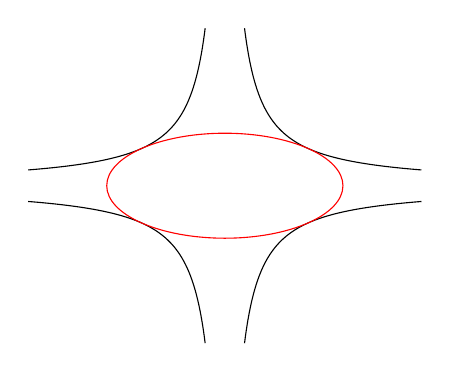
\begin{tikzpicture}[every node/.style={black}]
	\draw plot[variable=\x, samples=200,domain=0.25:2.5] ({\x},{1/(2*\x)});
	\draw plot[variable=\x, samples=200,domain=-0.25:-2.5] ({\x},{1/(2*\x)});
	\draw plot[variable=\x, samples=200,domain=0.25:2.5] ({\x},{-1/(2*\x)});
	\draw plot[variable=\x, samples=200,domain=-0.25:-2.5] ({\x},{-1/(2*\x)});
	\draw[red] (0,0) ellipse (1.5 and 0.666666);
\end{tikzpicture}
\end{center}
There seems to be enough symmetry here to say that the largest area an ellipse can obtain in the area between hyperbolas is $1$.
Especially since how well hyperbolas act when scaling the axes while maintaining area.

% Copyright 2024 Kieran W Harvie. All rights reserved.

\section{Barycentric Coordinates}
Let $P_k$ be the points of an $n$-simplex.
Then for any point $Q$ in the interior there exists a unique set of scalars $\lambda_k$ such that:
\begin{equation*}
\begin{aligned}
	0\leq&\lambda_k\\
	1=&\sum_{k=1}^n\lambda_n\\
	Q=&\sum_{k=1}^nP_n\lambda_n\\
\end{aligned}
\end{equation*}
These scalars are called the barycentric coordinates of the point $Q$.
In this section I will review the $n=2$ case, where the $n$-simplexes are triangles.

\subsection{Etymology}	
This is something that may be obvious to everyone but went over my head for a while.
The `bary' in barycentric isn't from someone named Bary,
but instead comes from the ancient Greek word `barús' meaning heavy,
similar to baryon.

\subsection{Triangles}
Given three 2D points $P_n$ why would we expect the set:
\[\{\lambda_1P_1+\lambda_2P_2+\lambda_3P_3|\lambda_1+\lambda_2+\lambda_3 = 1,\,\lambda_1 \geq 0,\,\lambda_2 \geq 0,\,\lambda_3 \geq 0\}\]
To have anything to do with triangles?
Well consider the function $f:\mathbb{R}^3\rightarrow\mathbb{R}^2$:
\[f(x,y,z) = P_1x+P_2y+P_3z\]
And consider the subset of $S\subset\mathbb{R}^3$ such that $x,y,z\geq0$ and $x+y+z=1$.
\\

$S$ is an equilateral triangle spanning the points $(1,0,0),\,(0,1,0)$ and $(0,0,1)$,
with the image of these points being the points $P_n$.
And $S$ is defined analogously the span of the barycentric coordinates,
so it's a good starting place to get some intuition.

\subsubsection{$f$ is linear}
This function is clearly linear:
\begin{equation*}
\begin{aligned}
	&f(ax_0+bx_1,ay_0+by_1,az_0+bz_1)\\
	=&P_1(ax_0+bx_1) + P_2(ay_0+by_1)+P_3(az_0+bz_1)\\
	=&a(P_1x_0+P_2y_0+P_3z_0) + b(P_1x_1+P_2y_1+P_3z_1)\\
	=&af(x_1,y_1,z_1)+bf(x_1,y_1,z_1)\\
\end{aligned}
\end{equation*}

\subsubsection{$f$ sends line segments to line segments}
Being linear means it sends line segments to lines segments (Or to a single point point if $f(A)=f(B)$):
\[f(At+B(1-t)) = f(A)t+f(B)(1-t)\] 
The function also keeps the `progress' along the line segment.
The point $Q=At+B(1-t)$ is $t$\% along the line $BA$ and $f(Q)$ is $t$\% along $f(B)f(A)$.

\subsubsection{$f$ is a bounded operator}
From the Cauchy-Schwartz inequality we can see that $f$ is a bounded operator:
\begin{equation*}
\begin{aligned}
	||f(\lambda_1,\lambda_2,\lambda_3)||
	=&(\lambda_1x_1+\lambda_2x_2+\lambda_3x_3)^2+(\lambda_1y_1+\lambda_2y_2+\lambda_3y_3)^2\\
	\leq&(\lambda_1^2+\lambda_2^2+\lambda_3^2)(x_1^2+x_2^2+x_3^2)+(\lambda_1^2+\lambda_2^2+\lambda_3^2)(y_1^2+y_2^2+y_3^2)\\
	=&(\lambda_1^2+\lambda_2^2+\lambda_3^2)(x_1^2+x_2^2+x_3^2+y_1^2+y_2^2+y_3^2)\\
\end{aligned}
\end{equation*}
For $(\lambda_1,\lambda_2,\lambda_3)\in S$ we have:
\[\lambda_1^2+\lambda_2^2+\lambda_3^2 \leq 1\]
meaning:
\[s\in S \Rightarrow ||f(s)|| \leq x_1^2+x_2^2+x_3^2+y_1^2+y_2^2+y_3^2\]
Hence all geometry in the image of $S$ takes place is a fixed circle around the origin.
While I don't think this result is technically necessary it does put my mind at ease about weird "projective geometry at infinity" edge cases.
\\

Curiously, 
we can make the inequality strict if we assume the triangle is non-degenerate.
Since there's equality in Cauchy-Schwartz iff:
\[k(x_1,x_2,x_3)=(\lambda_1,\lambda_2,\lambda_3)=l(y_1,y_2,y_3)\]
Which contradicts the triangle being non-degenerate.

\subsubsection{Interior}
Let $Q = (\lambda_1,\lambda_2,\lambda_3)\in S$ and $Q' = \frac{1}{\lambda_1+\lambda_2}(\lambda_1,\lambda_2,0)$, we can write:
\begin{equation*}
\begin{aligned}
	Q'=&\frac{\lambda_1}{\lambda_1+\lambda_2}(1,0,0)+\left(1-\frac{\lambda_1}{\lambda_1+\lambda_2}\right)(0,1,0)\\
	Q =& (1-\lambda_3)Q'+\lambda_3(0,0,1)\\
\end{aligned}
\end{equation*}
Which shows $Q'$ as being on the line segment $P_1P_2$ and $Q$ on $Q'P_3$:
\begin{center}
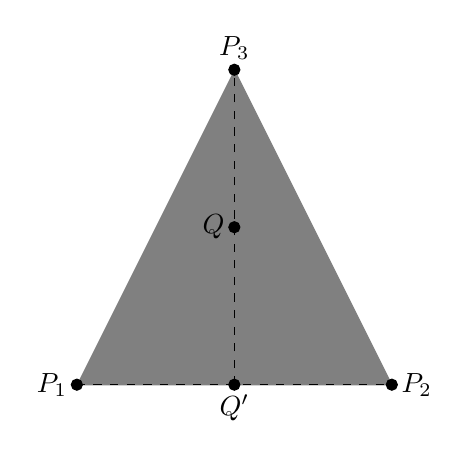
\begin{tikzpicture}[every node/.style={black}]
	\coordinate (P1) at (-2,0);
	\coordinate (P2) at (2,0);
	\coordinate (P3) at (0,4);

	\coordinate (Q') at (0,0);
	\coordinate (Q) at (0,2);

	\filldraw[gray] (P1) -- (P2) -- (P3);

	\draw[dashed] (P1) -- (P2);
	\draw[dashed] (Q') -- (P3);


	\filldraw (Q) node[left] {$Q$} circle (2pt);
	\filldraw (Q') node[below] {$Q'$} circle (2pt);
	\filldraw (P1) node[left] {$P_1$} circle (2pt);
	\filldraw (P2) node[right] {$P_2$} circle (2pt);
	\filldraw (P3) node[above] {$P_3$} circle (2pt);
\end{tikzpicture}
\end{center}
Because $Q'$ is on $P_1P_2$,
the opposite side to $P_3$,
$Q$ is on the segment between a point $P_3$ and that points opposite side $P_1P_2$ and hence is an interior point of $P_1P_2P_3$.
Hence $S\subset P_1P_2P_3$, 
this argument can be reversed to show that $P_1P_2P_3 \subset S$ and thus equality.
\\

Because of how $f$ preserves line segments,
the same stands for $f(Q')$ and $f(Q)$,
The same stands for $f(S) = f(P_1)f(P_2)f(P_3)$.

\subsection{Area coordinates}
\begin{center}
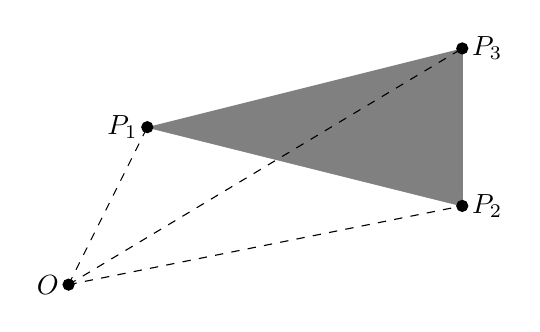
\begin{tikzpicture}[every node/.style={black}]
	\coordinate (O) at (0,0);
	\coordinate (P1) at (1,2);
	\coordinate (P2) at (5,1);
	\coordinate (P3) at (5,3);


	\filldraw[gray] (P1) -- (P2) -- (P3);

	\draw[dashed] (O) -- (P1);
	\draw[dashed] (O) -- (P2);
	\draw[dashed] (O) -- (P3);

	\filldraw (O) node[left] {$O$} circle (2pt);
	\filldraw (P1) node[left] {$P_1$} circle (2pt);
	\filldraw (P2) node[right] {$P_2$} circle (2pt);
	\filldraw (P3) node[right] {$P_3$} circle (2pt);
\end{tikzpicture}
\end{center}
The (unsigned) area of a triangle with points $P_1P_2P_3$ is given by:
\begin{equation*}
\begin{aligned}
	&\frac{1}{2}\left|\begin{vmatrix} x_1&x_2\\y_1&y_2\end{vmatrix} + \begin{vmatrix} x_2&x_3\\y_2&y_3 \end{vmatrix} + \begin{vmatrix} x_3&x_1\\y_3&y_1\end{vmatrix}\right|\\
	=&\frac{1}{2}(x_1(y_3-y_2)+x_2(y_1-y_3)+x_3(y_2-y_1))\\
\end{aligned}
\end{equation*}
This follows directly from the determinant being the signed area of the parallelogram spanned by its column vectors and can be rewritten, to isolate $P_1$, as:
\[\frac{1}{2}\big|x_1(y_3-y_2)-y_1(x_3-x_2)+x_3y_2-x_2y_3\big|\]
Let $Q$ have barycentric coordinates $(\lambda_1,\lambda_2,\lambda_3)$ and consider the area of the triangle $P_2P_3Q$:
\[\frac{1}{2}(\big|\lambda_1x_1+ \lambda_2x_2 + \lambda_3x_3)(y_3-y_2)-(\lambda_1y_1+ \lambda_2y_2 + \lambda_3y_3)(x_3-x_2)+x_3y_2-x_2y_3\big|\]
Considering just the first part shows that the like term, $x_ny_m$ where $n=m$, cancel to give:
\begin{equation*}
\begin{aligned}
	&(\lambda_1x_1+ \lambda_2x_2 + \lambda_3x_3)(y_3-y_2)-(\lambda_1y_1+ \lambda_2y_2 + \lambda_3y_3)(x_3-x_2)\\
	=&\lambda_1(x_1(y_3-y_2)-y_1(x_3-x_2))+ (\lambda_2x_2 + \lambda_3x_3)(y_3-y_2)-(\lambda_2y_2 + \lambda_3y_3)(x_3-x_2)\\
	=&\lambda_1(x_1(y_3-y_2)-y_1(x_3-x_2))+ \lambda_2(x_2y_3-x_3y_2) +\lambda_3(x_2y_3-x_3y_2)\\
	=&\lambda_1(x_1(y_3-y_2)-y_1(x_3-x_2))+ (1-\lambda_1)(x_2y_3-x_3y_2)\\
\end{aligned}
\end{equation*}
And hence and area of the triangle as:
\[\frac{\lambda_1}{2}\big|x_1(y_3-y_2)-y_1(x_3-x_2)+x_3y_2-x_2y_3\big|\]
This is why barycentric coordinates for triangles are also called area coordinates.
Because the first coordinate is the ratio of the area of the total triangle to $P_2P_3Q$,
and likewise for the other coordinates.
\\

% Trilinear conversion?

%The altitude of $P_1$ is perpendicular to $\overline{P_2P_3}$ giving it a gradient of:
%\[-\left(\frac{y_3-y_2}{x_3-x_2}\right)^{-1}= \frac{x_2-x_3}{y_3-y_2}\]
%Hence the foot lies at the intersection of:
%\begin{equation*}
%\begin{aligned}
%	0=&(y_3-y_2)(x-x_2)-(x_3-x_2)(y-y_2)\\
%	0=&(x_3-x_2)(x-x_1)+(y_3-y_2)(y-y_1)\\
%\end{aligned}
%\end{equation*}
%Giving the cool relations:
%\begin{equation*}
%\begin{aligned}
%	0=&(y_3-y_2)^2(x-x_2)+(x_3-x_2)^2(x-x_1)+(x_3-x_2)(y_3-y_2)(y_2-y_1)\\
%	0=&(x_3-x_2)^2(y-y_2)-(y_3-y_2)^2(y-y_1)+(x_3-x_2)(y_3-y_2)(x_2-x_1)\\
%\end{aligned}
%\end{equation*}
%

% Copyright 2024 Kieran W Harvie. All rights reserved.

\section{Partial Fractions}
Some observations and proofs of well known facts that I want to write down.

\subsection{Bézout's Identity}
Let $P_n$ be a finitely indexed family of polynomials and define:
\begin{equation*}
\begin{aligned}
Q_n =& \prod_{k\neq n}P_k\\
G =&\gcd(\{Q_n\}_n)\\
\end{aligned}
\end{equation*}
Then there exits polynomials $q_n$ such that:
\[\left(\prod_n P_n\right)^{-1} = G^{-1}\sum_n\frac{q_n}{P_n}\]
And that this solution is "the best we can get" in the sense that if there exits $q'_n$ and $G'$ such that:
\[\left(\prod_n P_n\right)^{-1} = G'^{-1}\sum_n\frac{q'_n}{P_n}\]
Then $\deg(G') \geq \deg(G)$

\subsubsection{Existence}
From Bézout's identity on $\{Q_n\}_n$ there existences $q_n$ such that:
\[\sum_n q_n Q_n = G \,\Rightarrow\, G^{-1}\sum_n q_n Q_n = 1\]
Substitution gives:
\begin{equation*}
\begin{aligned}
\left(\prod_n P_n\right)^{-1} =& \left(\prod_n P_n\right)^{-1}\left(G^{-1}\sum_n q_n Q_n\right)\\
=& G^{-1}\left(\sum_n q_n \left(\prod_{k\neq n} P_k\right)\left(\prod_k P_k\right)^{-1}\right)\\
=& G^{-1}\sum_n\frac{q_n}{P_n}\quad \square\\
\end{aligned}
\end{equation*}

\subsubsection{Best Case}
Assume we have $q_n'$ and $g'$ such that:
\[\left(\prod_n P_n\right)^{-1} = G'^{-1}\sum_n\frac{q'_n}{P_n}\]
Then doing all the previous steps in reverse gives:
\[\sum_n q_n' Q_n = G'\]
Meaning $G | G'$ and hence $\deg(G') \geq \deg(G)\quad\square$.

\subsubsection{Sharpness}
The above inequality is sharp,
this can be seen in the standard way.
Multiply the relevant polynomials by the same element $k$ from underlying ring gives a new solution with $\deg(G') = \deg(G)$:
\begin{equation*}
\begin{aligned}
	q'_n =& kq_n\\
	G' =& kG\\
\end{aligned}
\end{equation*}
We could, however, probably get some interesting results by putting some restrictions on $q_n$ and $P_n$.

\subsubsection{Remarks}
This result matches our intuition when calculating partial fractions,
that shared factors can't easily be removed:

If a polynomial $P$ can be factorized as $P=P_0P_1$ then:
\[\frac{1}{P} = \frac{1}{\gcd(P_0,P_1)}\left(\frac{q_0}{P_0}+\frac{q_1}{P_1}\right)\]
And the "Best Case" condition means we can't get rid of the external fraction.
\\

Also note that this result suggest the application of extended euclidean algorithm to partial fractions,
which sounds like it might be a fun one-day project.

\subsection{Divisibility}
What of the reverse?
If we have:
\[\frac{1}{P} = \frac{q_0}{P_0}+\frac{q_1}{P_1}\]
What can we say of the factorization of $P$?
Well the desired answer,
that $P_0$ and $P_1$ are factors of $P$,
doesn't work:
\[\frac{1}{x-1} = \frac{1}{x-2}-\frac{1}{(x-1)(x-2)}\]
The problem seems to come from cancellation means $P$ can be of lower degree then $P_0$ or $P_1$,
so lets take $\deg(P)$ as a possible condition.
\\

Simple manipulation gives:
\[(q_1P_0+q_0P_1)P = P_0P_1 = \lcm(P_0,P_1)\gcd(P_0,P_1)\]
Since $\gcd(P_0,P_1) | (q_1P_0+q_0P_1)$ we have $P | \lcm(P_0,P_1)$ meaning if $\deg(P) \geq \deg(\lcm(P_0,P_1))$ we have:
\[P = \lcm(P_0,P_1)\]

\subsubsection{Remark}
When preforming calculations we may not know $\deg(\lcm(P_0,P_1))$,
instead we can use $\deg(P) \geq \deg(P_0P_1)$ as:
\[\deg(P_0P_1) \geq \deg(\lcm(P_0,P_1))\]

\subsection{Complex Residue}
The application of the extended euclidean algorithm to finding the complex residues of rational functions is something I've talked about before.
But my prior attempts can be improved with these observations.
\\

Assume us want to find the residues of $P/Q$ at $a$ and $b$ where $Q$ has multiplicities $n$ and $m$.
Let $q$ be the polynomial such that:
\[Q(z) = q(z)(z-a)^n(z-b)^m\]
All three factors are pairwise relatively prime meaning there exists polynomials $s$,$r$, and $t$ such that:
\[s(z)(z-a)^nq(z)+r(z)(z-b)^mq(z)+t(z)(z-a)^n(z-b)^m = 1\]
Giving:
\[\frac{P(z)}{Q(z)} = s(z)\frac{P(z)}{(z-b)^m}+r(z)\frac{P(z)}{(z-a)^n}+t(z)\frac{P(z)}{q(z)}\]
Residues naturally follow.
Interestingly,
this approach might be able to to link the residues at $a$ and $b$ together.

\subsection{Perturbation}
I found this interesting perturbation identity while working:
\begin{equation*}
\begin{aligned}
	\frac{1}{(P_0-\lambda \delta_0)(P_1+\lambda \delta_1)} =& \frac{1}{P_0\delta_1+P_1\delta_0}\left(\frac{\delta_0}{P_0-\lambda \delta_0}+\frac{\delta_1}{P_1+\lambda \delta_1}\right)\\
	=&\frac{1}{P_0\delta_1+P_1\delta_0}\sum_{n=0}^{\infty}\lambda^n\left(\left(\frac{\delta_0}{P_0}\right)^{n+1}-\left(-\frac{\delta_1}{P_1}\right)^{n+1}\right)\\
\end{aligned}
\end{equation*}

This probably only has useful results when $\delta_0$ and $\delta_1$ are chosen such that $P_0\delta_1+P_1\delta_0$ means something.
Still cool.

% Copyright 2024 Kieran W Harvie. All rights reserved.

\section{Euler's Criterion}
Euler's criterion is and elementary number theory result that states that for odd prime $p$ and coprime non-zero integer $a$ we have:
\[x^{\frac{p-1}{2}}\mod p = \begin{cases} 1 & \text{ if $x$ is a square}\\ -1 & \text{ otherwise.}\end{cases}\]
I proved this the `involved' way back in the day,
but it's really easy to prove and generalize with field theory.

\subsubsection{Field Theory Proof:}
Let $p$ be an odd prime and consider the polynomial $q\in\mathbb{F}_p[X]$:
\[p(x) = x^{\frac{p-1}{2}}-1\]

\textbf{Lemma, every non-zero square is a root of $p$:}
Let $a=b^2$ then:
\[p(a) = p(b^2) = b^{p-1}-1 = 0\,\, \square\]

\textbf{Lemma, there are at least $\frac{p-1}{2}$ non-zero squares in $\mathbb{F}_p$:}
Let $a\in \mathbb{F}_p$ and consider the polynomial:
\[q(x) = x^2-a\]
There are at most two distinct roots of $q$ and when $a\neq 0$ any roots are non-zero.
However there are $p-1$ distinct non-zero elements of $\mathbb{F}_p$ and the square of every non-zero element is non-zero,
but no more than two can share the same value when squared,
hence there are at least $\frac{p-1}{2}$ non-zero squares in $\mathbb{F}_p$. $\square$
\\

Combining the previous results means every root of $p$ is distinct and a square.
The only loose end is to prove that $x^\frac{p-1}{2}=-1$ when $x$ isn't a square.
\\

From the previous result when $x$ isn't a square we know $x^\frac{p-1}{2}\neq 1$.
$0$ is a square, hence $x$ is non-zero meaning:
\[0 = x^{p-1}-1=\left(x^{\frac{p-1}{2}}-1\right)\left(x^{\frac{p-1}{2}}+1\right)\]
Since the first factor isn't zero the second must be,
giving $x^{\frac{p-1}{2}}=-1$, as required.
\\

This result easily generalizes to all finite fields of odd size.
Which are fields of odd prime characteristic,
cool.

\subsubsection{Low Hanging Generalizations:}
Let $\mathbb{F}_n$ be a finite field and suppose $n-1$ is divisible by $m$ and let:
\[p(x) = x^\frac{n-1}{m}-1\]
Similar arguments show that all the roots of $p$ are distinct and are the non-zero $m$th powers.
Now it's only the loose ends of non-powers that matter.
\\

Let $h$ be an element of order $m$.
(Guaranteed since every finite field has a generator $g$ which you can raise to power $g^\frac{n-1}{m}$).
And let $q$ be:
\[q(x)=x^m-1\]
From similar arguments as those above,
you can show that the powers of $h$ are the roots of $q$:
\[q(x) = x^m-1= \prod_{k=1}^m(x-h^k)\]
Substitute $x\mapsto x^\frac{n-1}{m}$ to give:
\[\prod_{k=1}^m(x^\frac{n-1}{m}-h^k)= (x^\frac{n-1}{m})^m-1=x^{n-1}-1\]
Hence for non-zero $x$ we have:
\[\prod_{k=1}^m(x^\frac{n-1}{m}-h^k)= 0\]
Meaning $x^\frac{n-1}{m}$ is a power of $h$.
\\

We can combine these results in a nice way:
Let $m$ divide $n-1$ and let $h$ be an element of order $m$.
Define $f_m:\mathbb{F}_n^\times\rightarrow \langle h\rangle \cong C_m$ such that $f_m(x) = x^{\frac{n-1}{m}}$
$f_m$ is a group homomorphism where the kernel is the $m$th powers of $\mathbb{F}_n$

%Suppose $n-1$ is divisible by $3$ and let $h$ be an element of order $3$.
%(Guaranteed since every finite field has a generator $g$ which you can raise to power $g^\frac{n-1}{3}$).
%We have:
%\begin{equation*}
%\begin{aligned}
%&\left(x^\frac{n-1}{3}-1\right)\left(x^\frac{n-1}{3}-h\right)\left(x^\frac{n-1}{3}-h^2\right)\\
%=&x^{n-1}-x^\frac{2(n-1)}{3}\left(1+h+h^2\right) +x^\frac{n-1}{3}\left(1\cdot h+1\cdot h^2+h\cdot h^2\right)-1\cdot h\cdot h^2\\
%=&x^{n-1}-1\\
%\end{aligned}
%\end{equation*}
%Easy to see that:
%\[\img\left(x^\frac{n-1}{m}\right)=\langle h \rangle \cong C_3\]
%and
%\[\ker\left(x^\frac{n-1}{m}\right)=\{\text{$m$th powers}\}\]
%
%Unfortunately this doesn't work for $4$ and I'll have to actually think,
%will probably use:
%\[\ord(x^k) = \frac{\ord(x)}{\gcd(k,\ord(x))}\]

% Copyright 2024 Kieran W Harvie. All rights reserved.

\section{p-adic Acceleration}
Say we are part way through calculating the p-adic expansion of $\frac{1}{n}$ and have:
\[\frac{1}{n} = a_0+a_1p^1+a_2p^2+\dots+a_{k-1}p^{k-1}+rp^{k}\frac{1}{n}\]
Then we have:
\begin{equation*}
\begin{aligned}
\frac{1}{n} =& a_0+a_1p^1+a_2p^2+\dots+a_{k-1}p^{k-1}+rp^{k}\frac{1}{n}\\
=& a_0+a_1p^1+a_2p^2+\dots+a_{k-1}p^{k-1}+rp^{k}\left(a_0+a_1p^1+a_2p^2+\dots+a_{k-1}p^{k-1}+rp^{k}\frac{1}{n}\right)\\
=& a_0+a_1p^1+a_2p^2+\dots+a_{k-1}p^{k-1}+a_0rp^{k}+a_1rp^{k+1}+a_2rp^{k+2}+\dots+a_{k-1}rp^{2k-1}+r^2p^{2k}\frac{1}{n}\\
\end{aligned}
\end{equation*}

Observe that,
after we clean up the multiplication of coefficients by $r$,
we have doubled the number of coefficients.
\\

Unfortunately,
despite getting the unclean coefficients being $O(\log(N))$ cleaning the coefficients is still $O(N)$.
Where $N$ is the number of desired coefficients.

\subsubsection{Example:}
Consider $n=1000$ and $p=7$.
User Bézout's identity to get the initial value:
\[(-857 )\times7+6\times1000=1\Rightarrow \frac{1}{1000} = 6-\frac{857}{1000}7\]
First iteration:
\[\frac{1}{1000}=6-5142\times7+734449\times7^2\times\frac{1}{1000}\]
Example cleanup:
\begin{equation*}
\begin{aligned}
\frac{1}{1000}=&6+(735\times7-5142\times-735\times7)7+734449\times7^2\times\frac{1}{1000}\\
=&6+3\times7+(734449-735\times1000)\times7^2\times\frac{1}{1000}\\
=&6+3\times7-551\times7^2\times\frac{1}{1000}\\
\end{aligned}
\end{equation*}
Second iteration:
\begin{equation*}
\begin{aligned}
\frac{1}{1000}=&6+3\times7-551\times7^2\times\left(6+3\times7-551\times7^2\times\frac{1}{1000}\right)\\
=&6+3\times7+5\times7^2-2126\times7^3+303601\times7^4\frac{1}{1000}\\
=&6+3\times7+5\times7^2+2\times7^3-399\times7^4\frac{1}{1000}\\
\end{aligned}
\end{equation*}
We got the coefficient of $7^3$ and well as $7^2$.



\chapter{2023}
% Copyright 2023 Kieran W Harvie. All rights reserved.

\section{Laplace Expansion}
The Laplace Expansion is a way to compute the determinate of an $n\times n$ matrix in term of $(n-1)\times (n-1)$ determinates.
It's also kind of hard to cleanly state without some terminology I'll introduce later,
but the gist can be found in the $n\in\{2,3\}$ examples:
\[\begin{vmatrix} a&b&c\\d&e&f\\g&h&i\\ \end{vmatrix} =
	a\begin{vmatrix} e&f\\h&i\end{vmatrix}
	-b\begin{vmatrix}d&f\\g&i\end{vmatrix}
	+c\begin{vmatrix}d&e\\g&h\end{vmatrix}
\]
and:
\[\begin{vmatrix} a&b\\ c&d\\ \end{vmatrix} = a|d|-b|c| = ad-bc 
\]
(Note that in the second expression $|\cdot|$ is the determinate of a $1\times 1$ matrix and not absolute value.)

This seems like a good way to define the determinate,
something I have been working on
\footnote{Yes I know the geometric characterization, 
I'm just not looking for that right now.},
so with this definition I wish to understand:

\begin{itemize}
	\item Why it is well defined, meaning that we can expand along different rows columns.
	\item Elementary row operations.
	\item Product rule.
	\item Triangle rule.
	\item Inverse matrix in terms of the cofactor.
	\item Relation to the Wedge product.
\end{itemize}

\subsection{Terminology}
For a given $m\times n$ matrix $A$ the entries $a_{i,j}$ are arranged such that:
\[\begin{bmatrix}
	a_{1,1}&a_{1,2}&\dots&a_{1,n} \\
	a_{2,1}&a_{2,2}&\dots&a_{2,n} \\
	\vdots&\vdots&\ddots&\vdots\\
	a_{m,1}&a_{m,2}&\dots&a_{m,n} \\
\end{bmatrix}\]

\subsubsection{Principal Diagonal}
The principal diagonal of a matrix are the elements $a_{i,j}$ such that $i=j$. 
\[\begin{bmatrix}
	\color{red} a_{1,1}&a_{1,2}&a_{1,3}&a_{1,4} \\
	a_{2,1}&\color{red} a_{2,2}&a_{2,3}&a_{2,4} \\
	a_{3,1}&a_{3,2}&\color{red} a_{3,3}&a_{3,4} \\
	a_{4,1}&a_{4,2}&a_{4,3}&\color{red} a_{4,4} \\
\end{bmatrix}\]
Sometimes also called the "main diagonal".

\subsubsection{Submatrix}
A submatrix is a subset of rows and column and can look quite different depending on how the rows/columns are chosen.
For example both:
\[
\begin{bmatrix}
	\color{red} a_{1,2} \\
	\color{red} a_{2,2} \\
\end{bmatrix}
\quad\text{and}\quad
\
\begin{bmatrix}
	\color{blue} a_{1,1}&\color{blue} a_{1,3}&\color{blue} a_{1,4} \\
	\color{blue} a_{2,1}&\color{blue} a_{2,3}&\color{blue} a_{2,4} \\
	\color{blue} a_{4,1}&\color{blue} a_{4,3}&\color{blue} a_{4,4} \\
\end{bmatrix}\]
Are submatrices of:
\[\begin{bmatrix}
	\color{blue} a_{1,1}&\color{red} a_{1,2}&\color{blue} a_{1,3}&\color{blue} a_{1,4} \\
	\color{blue} a_{2,1}&\color{red} a_{2,2}&\color{blue} a_{2,3}&\color{blue} a_{2,4} \\
	a_{3,1}&a_{3,2}&a_{3,3}&a_{3,4} \\
	\color{blue} a_{4,1}&a_{4,2}&\color{blue} a_{4,3}&\color{blue} a_{4,4} \\
\end{bmatrix}\]
Where in the first one the subset was rows $1$ and $2$ and column $1$ making the block contiguous in the main matrix.
Where for the second one we took all except rows $3$ and column $2$, effectively cutting them out.

\subsubsection{Minor}
The minor $M_{i,j}$ of an element $a_{i,j}$ is the determinate of the submatrix where the row and column are removed.
Given:
\[\begin{bmatrix}
	a_{1,1}&a_{1,2}&a_{1,3}&a_{1,4} \\
	a_{2,1}&a_{2,2}&a_{2,3}&a_{2,4} \\
	a_{3,1}&a_{3,2}&a_{3,3}&a_{3,4} \\
	a_{4,1}&a_{4,2}&a_{4,3}&a_{4,4} \\
\end{bmatrix}\]
The minor $M_{3,2}$ is given by:
\[M_{3,2} = \begin{vmatrix}
	a_{1,1}&a_{1,3}&a_{1,4} \\
	a_{2,1}&a_{2,3}&a_{2,4} \\
	a_{4,1}&a_{4,3}&a_{4,4} \\
\end{vmatrix}\]

\subsubsection{Minor of General Order}
There is a more general definition of a minor that isn't used in the definition of Laplace Expansion,
but will be used in proofs.
\\

Let $I$ and $J$ be a set of integers between $1$ and $n$ such that the submatrix with all $I$ rows and $J$ columns are removed is a $k\times k$ matrix.
Then the determinate of the submatrix is denoted $M_{I,J}$ and is called a `minor of order $k$'.
\\


The minor $M_{\{1,3\},\{1,2\}}$ is of order $2$ and is given by:
\[M_{\{1,3\},\{1,2\}} = \begin{vmatrix}
	a_{2,3}&a_{2,4} \\
	a_{4,3}&a_{4,4} \\
\end{vmatrix}\]
The minor $M_{\{1,2,3\},\{1,2,4\}}$ is of order $1$ and is given by:
\[M_{\{1,2,3\},\{1,2,4\}} = \begin{vmatrix}
	a_{4,3} \\
\end{vmatrix} = a_{4,3}\]
Some important observations before continuing:
\begin{itemize}
	\item As expected, $M_{\{i\},\{j\}} = M_{i,j}$ and the previous minor can be called the "minor of order $n-1$" or "first minor".
	\item We have the base cases $M_{\varnothing,\varnothing} = |A|$ and $M_{\{1,2,\ldots,i-1,i+1,\ldots n\},\{1,2,\ldots,j-1,j+1,\ldots n\}} = a_{i,j}$.
	\item This definition can be extended to non-square matrices, provided the submatrix with all $I$ rows and $J$ columns removed is a square $k\times k$ matrix everything still works.
		$I$ and $J$ just wont have the same number of elements.
\end{itemize}

\subsubsection{Cofactor}
The cofactor $C_{i,j}$ of an element $a_{i,j}$ is the minor of that element multiplied by $(-1)^{i+j}$.
The cofactor of $a_{3,2}$ of the previous example is given by:
\[C_{3,2} = (-1)^5\begin{vmatrix}
	a_{1,1}&a_{1,3}&a_{1,4} \\
	a_{2,1}&a_{2,3}&a_{2,4} \\
	a_{4,1}&a_{4,3}&a_{4,4} \\
\end{vmatrix}= -\begin{vmatrix}
	a_{1,1}&a_{1,3}&a_{1,4} \\
	a_{2,1}&a_{2,3}&a_{2,4} \\
	a_{4,1}&a_{4,3}&a_{4,4} \\
\end{vmatrix}\]

\subsection{Laplace Expansion}
Laplace Expansion states that you can find the determinate of a matrix by the sum of the elements in a row/column times by their cofactor.
Expanding along the $j$th column gives:
\[|A| = \sum_{i=1}^na_{i,j}C_{i,j}\]
Like wise for the $i$th row:
\[|A| = \sum_{j=1}^na_{i,j}C_{i,j}\]
If we include the base case that the determinate of a $1\times 1$ matrix is its sole element,
this actually serves as a definition of the determinate.

\subsubsection{Well Definedness of Row/Column}
Well definedness of columns requires showing that the following expression is independent of $j$:
\[|A| = \sum_{i=1}^na_{i,j}(-1)^{i+j}M_{i,j}\]
The idea of the proof is simple induction.
Show its true for $n\leq 2$
then prove for $n>2$ with $j_0\neq j_1$ by expanding along $j_0$ then $j_1$ and $j_1$ then $j_0$ and comparing the two results.
\\

\textit{The determinate of dimension $1$ and $2$ are well defined:}
For dimension $1$ there is one element and hence are well defined.
For dimension $2$ have we have:
\[|A| = \begin{vmatrix} a_{1,1} & a_{1,2}\\a_{2,1} & a_{2,2}\end{vmatrix}\]
Expand on the first column to give:
\[|A| = a_{1,1}|a_{2,2}|-a_{1,2}|a_{2,1}| = a_{1,1}a_{2,2}-a_{1,2}a_{2,1}\]
And likewise on the second column to give:
\[|A| = -a_{2,1}|a_{1,2}|+a_{2,2}|a_{1,1}| = a_{1,1}a_{2,2}-a_{1,2}a_{2,1}\]

\textit{Determinates of dimension greater than $2$:}
Let $j_0>j_1$ be indexes of columns in $A$ and expand $|A|$ on the larger $j_0$th column first:
\[|A| = \sum_{i_0=1}^na_{i_0,j_0}(-1)^{i_0+j_0}M_{i_0,j_0}\]
By the inductive assumption the determinate is well defined for the for any column of the submatrix defining $M_{i_0,j_0}$.
Expanding on $j_1$ gives:
\begin{equation*}
	\begin{aligned}
		M_{i_0,j_0}=&\sum_{i_1=1}^{i_0-1}(-1)^{i_1+j_1}a_{i_1,j_1}M_{\{i_0,i_1\},\{j_0,j_1\}}+\sum_{i_1=i_0+1}^{n}(-1)^{i_1+j_1-1}a_{i_1,j_1}M_{\{i_0,i_1\},\{j_0,j_1\}}\\
		=&\sum_{i_1=1}^{i_0-1}(-1)^{i_1+j_1}a_{i_1,j_1}M_{\{i_0,i_1\},\{j_0,j_1\}}-\sum_{i_1=i_0+1}^{n}(-1)^{i_1+j_1}a_{i_1,j_1}M_{\{i_0,i_1\},\{j_0,j_1\}}\\
	\end{aligned}
\end{equation*}

The split sum is because when $i_1>i_0$ a prior row has been removed in making the submatrix,
so we have to move the elements up one,
which factors out to a multiplication by $-1$.
No such modification is required for the column because we assume $j_1<j_0$,
if we had chosen $j_1 > j_0$ the whole expression would have been multiplied by $-1$.
\\

Observe that the left term is positive and has matching $i_1< i_0$ and $j_1 < j_0$ while the right term is negative and has mismatched $i_1> i_0$ and $j_1 < j_0$.
If we had expanded along the smaller $j_1$ first the whole expression would gain a $-1$ making the left term negative and the right positive but the left would have mismatched $i_1< i_0$ and $j_1 > j_0$ while the right would have matching $i_1 > i_0$ and $j_1 > j_0$.
Hence pairing of sign and matched-ness stay the same.
\\

This is what causes both orders of expansion to be the same and the well definedness for columns,
as can be seen when substituting the above expression back into the Laplace Expansion for $|A|$ and changing the order of summation such that the larger row is the outer summation:
\begin{equation*}
\begin{aligned}
	|A|=&\sum_{i_0=1}^{n}(-1)^{i_0+j_0}a_{i_0,j_0}M_{i_0,j_0} \\
	=&\sum_{i_0=1}^{n}(-1)^{i_0+j_0}a_{i_0,j_0}\bigg(
		\sum_{i_1=1}^{i_0-1}(-1)^{i_1+j_1}a_{i_1,j_1}M_{\{i_0,i_1\},\{j_0,j_1\}}\\
		&\quad+\sum_{i_1=i_0+1}^{n}(-1)^{i_1+j_1+1}a_{i_1,j_1}M_{\{i_0,i_1\},\{j_0,j_1\}}
	\bigg) \\
	=&\sum_{i_0=1}^{n}\sum_{i_1=1}^{i_0-1}(\overbrace{a_{i_0,j_0}a_{i_1,j_1}}^\text{Matched}-\overbrace{a_{i_1,j_0}a_{i_0,j_1}}^\text{Mismatched})(-1)^{i_0+i_1+j_0+j_1}M_{\{i_0,i_1\},\{j_0,j_1\}} \\
\end{aligned}
\end{equation*}

Expanding $j_1$ first would have multiplied the expression for the minor by $-1$ but make the outer factor ($a_{i_0,j_1}$) mismatched.
When changing the order of summation,
such that the larger row is the outer summation,
this $-1$ would sill get paired with the mismatched term.
Hence we get the same result regardless of if the smaller or larger column is expanded first,
as required.
\\

Note that this argument can be recycled for rows.
Also note that the final summed term is symmetric in $j_0$ and $j_1$,
maybe a closing argument can come from this symmetry.

\subsubsection{Well Definedness of Direction}
From the previous section we know the following expressions are independent of $k$:
\[|A|_r = \sum_{i=1}^na_{i,k}C_{i,k},\quad |A|_c = \sum_{i=1}^na_{k,i}C_{k,i}\]
Define:
\[S=\frac{1}{n}\sum_{j=1}^n\sum_{i=1}^na_{j,i}C_{j,i}\]
We have:
\[S=\frac{1}{n}\sum_{j=1}^n\sum_{i=1}^na_{j,i}C_{j,i} = \frac{1}{n}\sum_{j=1}^{n}|A|_c = |A|_c\]
However, the finitude of the summation means we can reverse the order to similarly give:
\[S=|A|_r\]
Hence:
\[|A|_r = S = |A|_c\]
As required.

\subsection{Triangular Matrix}
A lower triangular matrix is one where $i<j \Rightarrow a_{i,j} = 0$.
They are called such because when written out in matrix form they look like a triangle:
\[\begin{bmatrix}
	a_{1,1}&a_{1,2}&a_{1,3}&a_{1,4} \\
	a_{2,1}&a_{2,2}&a_{2,3}&a_{2,4} \\
	a_{3,1}&a_{3,2}&a_{3,3}&a_{3,4} \\
	a_{4,1}&a_{4,2}&a_{4,3}&a_{4,4} \\
\end{bmatrix} =
\begin{bmatrix}
	a_{1,1}&0&0&0 \\
	a_{2,1}&a_{2,2}&0&0 \\
	a_{3,1}&a_{3,2}&a_{3,3}&0 \\
	a_{4,1}&a_{4,2}&a_{4,3}&a_{4,4} \\
\end{bmatrix}\]
The upper triangular matrix is the reverse with $i>j \Rightarrow a_{i,j} = 0$.
\\

By induction the determinate of a lower triangular matrix is the product of all principal diagonal elements.
The base case is a matrix of size $1\times 1$ and true by definition. 
In the induction step observe that the only nonzero element in the $1$st row is $a_{1,1}$ hence:
\[|A| = a_{1,1}C_{1,1} = a_{1,1}M_{1,1}\]
The submatrix used for $M_{1,1}$ is a lower diagonal matrix with all principle elements but $a_{1,1}$
Hence:
\[M_{1,1} = a_{2,2}a_{3,3}\dots a_{n,n}\]
Giving:
\[|A| = a_{1,1}a_{2,2}a_{3,3}\dots a_{n,n}\]
As required.
\\

I've included a more visual proof bellow:
\[\begin{vmatrix}
	a_{1,1}&0&0&\dots&0 \\
	a_{2,1}&a_{2,2}&0&\dots&0 \\
	a_{3,1}&a_{3,2}&a_{3,3}&\dots&0 \\
	\vdots&\vdots&\vdots&\ddots&\vdots \\
	a_{n,1}&a_{n,2}&a_{n,3}&\dots&a_{n,n} \\
\end{vmatrix}
=a_{1,1}
\begin{vmatrix}
	a_{2,2}&0&\dots&0 \\
	a_{3,2}&a_{3,3}&\dots&0 \\
	\vdots&\vdots&\ddots&\vdots \\
	a_{n,2}&a_{n,3}&\dots&a_{n,n} \\
\end{vmatrix}
=a_{1,1}a_{2,2}a_{3,3}\dots a_{n,n}\]

\subsection{Product Rule}
We wish to show that:
\[|AB|=|A||B|\]
This will be useful for analysing other properties of the determinate because if we can find a matrix representing that operation we can simply times by that matrix's determinate.
\\

We will have to deal with multiple cofactor so use that notation:
\[C[A]_{i,j}\]
For the $(i,j)$th cofactor of matrix $A$.
Maybe move this notation into the terminology section.

\subsection{Permutation Matrix}
A permutation matrix is a matrix where each row and each column have exactly one non-zero element and every non-zero element is equal to $1$.
\\

Let $\pi:\mathbb{N}\rightarrow\mathbb{N}$ be a function where $\pi(n)$ is the column of the non-zero element it the $n$th row.

\[S=n+\sum_{k=1}^n\pi(k)-\sum_{k=1}^{n}|\{j<k \text{ where } \pi(j)<\pi(k)\}|\]
Then the determinate is $(-1)^S$

% Copyright 2023 Kieran W Harvie. All rights reserved.

\section{Finite Field Endofunctions}
Let $F_n$ be and finite field and let $f$ be an endofunction,
then $f$ can be written as a polynomial of degree $n-1$ or less.
\\

Construct an indicator function in the normal way:
\[\chi_y(x) = \prod_{z\in F_n/\{y\}}\frac{x-z}{y-z}\]
Observe that this is a $n-1$ degree polynomial.
Now use the indicator function in the normal way:
\[f(x) = \sum_{y\in F_n}\chi_y(x)f(y)\]

\subsection{Low Hanging Fruit}
\[f(x) = yx\]
For non-zero $y$,
this is a permutation of $F_n$ that only fixes $0$.
\[f(x) = x+y\]
Is a permutation that doesn't fix anything.
Combining the two gives:
\[f(x) = y(x-x_0)+x_0\]
A permutation that only fixes $x_0$.

\subsection{Elementary Symmetric Function}
Let $e_n(S)$ be the $n$th elementary symmetric function of the set $S$ with element $y$.
\[e_0(S) = 0\]
\[e_n(S/\{y\})=e_n(S)-ye_{n-1}(S/\{y\})\]
\[e_n(S/\{y\})=\sum_{k=0}^ne_k(S)(-y)^{n-k}\]
Now recall:
\[x^{n}-x = \prod_{y\in F_n}(x-y)\]
Which gives the classic:
\[e_m(F_n) = \begin{cases} 1 & m = 0\text{ or } m = n-1\\ 0 & \text{ else}\\\end{cases}\]
\\

The first simplification we can make is to notice that:
\begin{equation*}
\begin{aligned}
\prod_{z\in F_n/\{y\}}\frac{1}{y-z} =& \frac{1}{e_{n-1}(F_n/\{0\})}\\
=& \frac{1}{e_{n-1}(F_n)-0e_{n-2}(F_n/\{0\})}\\
=&1\\
\end{aligned}
\end{equation*}
Hence:
\[\chi_y(x) = \prod_{z\in F_n/\{y\}}(x-z)\]
Going further:
\begin{equation*}
\begin{aligned}
e_m(F_n/\{y\})=&\sum_{k=0}^me_k(F_n)(-y)^{m-k}\\
=&(-y)^m+[m\geq n-1](-y)^{m-(n-1)}\\
\end{aligned}
\end{equation*}

\begin{equation*}
\begin{aligned}
\chi_y(x) =& \prod_{z\in F_n/\{y\}}(x-z)\\
=&\sum_{k=0}^{n-1}x^k(-1)^{n-k-1}e_{n-k-1}(F_n/\{y\})\\
=&\sum_{k=0}^{n-1}x^k(-1)^{n-k-1}(-y)^{n-k-1}+(-1)^{n-1}\\
=&\sum_{k=0}^{n-1}x^ky^{n-k-1}+(-1)^{n-1}\\
\end{aligned}
\end{equation*}
Which I guess makes a lot of sense when looked at like a geometric progression with
Frobenius to the numerator.
But that this more formal argument is cool.

\subsection{Second Attempt}
The last attempt with elementary polynomials had errors and was generally sloppy,
but it's enough to work backwards from:
\[\chi_y(x) = \frac{1}{n-1}\sum_{k=0}^{n-2}x^ky^{n-1-k}+y^{n-1}\frac{x^{n-1}-1}{n-1}+(1-x^{n-1})(1-y^{n-1})\]
When $y=0$ we have:
\[\chi_y(x) = 1-x^{n-1}\]
When $y\neq 0$ we have:
\[\chi_y(x) = \frac{1}{n-1}\sum_{k=0}^{n-2}(xy^{-1})^k+\frac{x^{n-1}-1}{n-1}\]
Gives Fourier vibes, might try again with generators.
\\

On further reflection:
\begin{equation*}
\begin{aligned}
	\chi_y(x) =& \frac{1}{n-1}\sum_{k=0}^{n-2}(xy^{-1})^k+\frac{x^{n-1}-1}{n-1}\\
	=& \frac{1}{n-1}\sum_{k=1}^{n-1}(xy^{-1})^k\\
\end{aligned}
\end{equation*}
So yea, Fourier.

\subsection{Polynomial}
\[f(x) = \frac{1}{n-1}\sum_{k=1}^{n-1}x^k\sum_{y\in F_n/\{0\}}\frac{f(y)}{y^k}+f(0)(1-x^{n-1})\]
If we write:
\[\hat{f}(k)=\sum_{y\in F_n/\{0\}}f(y)y^{-k}\]
Then the Fourier transform becomes even more apparent,
especially if rephrased in terms of a generator,
which is a cool result.
\\

Also note that a endomorphism will have $f(0)=0$ and remove the annoying edge case.

% Copyright 2023 Kieran W Harvie. All rights reserved.

\section{Vieta's Formula Applied to Prime Fields}
For a prime number $p$ we have the well known formula:
\[x^p-x \equiv \prod_{k=0}^{p-1}(x-k)\,\mod p\]
(Look up Frobenius Endomorphism for more info).

Vieta's formulas link the elementary symmetric functions of a polynomials roots to it's polynomials.
There are two nonzero coefficients the $p$-th degree doesn't tell anything and the $1$ is one-half of Wilson's Theorem:
\[(p-1)! \equiv -1\,\mod p\]

The other coefficients are zero hence the other elementary symmetric functions of $0$ to $p-1$ are divisible by $p$.
(Since terms with $0$ vanish $1$ to $p-1$ can be used).

\subsubsection{Example $p=5$:}
\begin{equation*}
\begin{aligned}
	&1\cdot2\cdot3\cdot 4 &=& 24 =&&5\cdot5-1\\
	&1\cdot2\cdot3 + 1\cdot2\cdot4+1\cdot3\cdot4+2\cdot3\cdot4&=& 50 =&& 5\cdot 10\\
	&1\cdot2+1\cdot3+1\cdot4+2\cdot3+2\cdot4+3\cdot4 &=& 35 =&&5\cdot 7\\
	&1+2+3+4 &=& 10 =&&5\cdot 2\\
\end{aligned}
\end{equation*}

\subsection{Commutative Rings}
Let $R$ be a commutative ring and let $x_0$ and $x_1$ be distinct elements of $R$.
Let $f$ be an element of $R[X]$ such that $f(x_0)=f(x_1) = 0$ then:
\[f(x) = (x-x_0)(x-x_1)q(x)+(x-x_0)r\]
For some $r\in R$ and $q \in R[X]$.
\\

\subsubsection{Proof:}
It is a corollary of Euclidean division of polynomials with monic polynomials that for a given $p\in R[X]$ and $x'\in R$ there exists a $p' \in R[X]$ such that:
\[p(x) = (x-x')p'(x)+p(x')\]
Applying this to $f$ and $x_0$ we get:
\[f(x) = (x-x_0)f'(x) + f(x_0) = (x-x_0)f(x)\]
And applying this to $f'$ and $x_1$ we get:
\[f(x) = (x-x_0)((x-x_1)f''(x)+f'(x_1))\]
Setting $q=f''$ and $r=f'(x_1)$ completes the proof

\subsubsection{Corollary:}
If $R$ is a domain, 
has no zero dividers,
then $r=0$ since $x_1-x_0\neq 0$ and:
\[0 = f(x_1) = (x_1-x_0)r\]
This is why the result main result works since $\mathbb{Z}/p\mathbb{Z}$ is a field,
and hence domain,
and why it may not work in general as:
\[2\cdot 3 \equiv 0 \mod 6\]

\subsection{Composite Numbers}
For general $n$ and relative prime $x$ we have:
\[x^{\lambda(n)}\equiv 1 \mod n\]
Which looks similar but we already see problems.
There are $\phi(n)$ totients to $n$ but $\lambda(n)$ can be less than $\phi(n)$ meaning a $\lambda(n)$ degree polynomial with $\phi(n)$ distinct roots has more roots than it's degree.
For example:
\[\lambda(8) = 2 < 4 = \phi(8)\]
So all of $\{1,3,5,7\}$ are roots of:
\[x^2-1 \mod 8\]

\subsubsection{Notes}
Considering the case $n=15$ since it's the lowest number with $2<\lambda(n)<\phi(n)$ as $\lambda(15) = 4$ and $\phi(15) = 8$.

\[x^4-1 = (x-1)(x-2)(x^2+3x+7)\]
\[x^4-1 = (x-1)(x-14)(x^2+1)\]
\[x^4-1 = (x-1)(x-8)(x^2+9x+13)\]

% Copyright 2023 Kieran W Harvie. All rights reserved.

\section{Harmonic Mean Probability}
Cool little result,
let there be a binary categorical random veritable with a probability $p$ of being $1$ and $1-p$ of being $0$.
Then we have the cool result:
\[\frac{\Pr(10)+\Pr(01)}{\Pr(11)+\Pr(00)} = \frac{2p(1-p)}{p^2+(1-p)^2} = \frac{2}{\frac{p}{1-p}+\frac{1-p}{p}}\]
The ratio of the chance of two dissimilar results to two similar results is the harmonic mean of $\frac{p}{1-p}$ and it's reciprocal.
\\

Neat.

% Copyright 2023 Kieran W Harvie. All rights reserved.

\section{Iverson Bracket and Möbius Function}
I saw a pretty cool manipulation the other day.
Let $f$ be a function such that:
\[f(da,db) = g(d)h(a,b)\]
Then we can "factor out" a relative prime condition in a cool way:
\[\sum_{\substack{a,b > 0\\ \gcd(a,b) = 1}}f(a,b) = \left(\sum_{d>0}\mu(d)g(d)\right)\left(\sum_{a,b>0}h(a,b)\right)\]
Where $\mu$ is the Möbius function.
I won't be going into it here,
just know there are a lot of known sums that make the first term of the RHS tractable:
\\

\begin{tabular}{|c|c|c|c|c|c|c|}
\hline
	$g(n)$&$n^{-s}$&$n^{-1}$&$\ln(n)n^{-1}$&$\ln(n)^2n^{-1}$&$q^n(1-q^n)^{-1}$&$\mu(n)n^{-s}$\\
	\hline
	$\sum_{n>0}\mu(n)g(n)$&$\zeta(n)^{-1}$&$0$&$1$&$-2\gamma$&$q$&$\zeta(s)\zeta(2s)^{-1}$\\
	\hline
\end{tabular}
\\

To prove this consider the well known result:
\[\sum_{d|n}\mu(d) = \begin{cases} 1&n=1\\ 0&\text{else} \end{cases}\]
And the Iverson bracket,
notation I normally think is ugly but is cool here,
where for a true or false proposition $P$ we define:
\[[P] = \begin{cases} 1 & P \text{ is true} \\ 0 & P \text{ is false} \end{cases}\]
(Basically an indicator function, or like typecasting from programing).
We have:
\begin{equation*}
\begin{aligned}
[\gcd(a,b)=1] =&
\sum_{d|\gcd(a,b)}\mu(d)\\
=&\sum_{d>0}[d|\gcd(a,b)]\mu(d)\\
=&\sum_{d>0}[d|a \cap d|b]\mu(d)\\
=&\sum_{d>0}[d|a][ d|b]\mu(d)\\
\end{aligned}
\end{equation*}

Hence:
\begin{equation*}
\begin{aligned}
\sum_{\substack{a,b > 0\\ \gcd(a,b) = 1}}f(a,b) =& \sum_{a,b>0}[\gcd(a,b)=1]f(a,b)\\
=&\sum_{a,b>0}\left(\sum_{d>0}[d|a][d|b]\mu(d)\right)f(a,b) \\
=&\sum_{d>0}\mu(d)\sum_{a,b>0}[d|a][d|b]f(a,b) \\
=&\sum_{d>0}\mu(d)\sum_{a,b>0}f(da,db) \\
=&\sum_{d>0}\mu(d)\sum_{a,b>0}g(d)h(a,b) \\
=& \left(\sum_{d>0}\mu(d)g(d)\right)\left(\sum_{a,b>0}h(a,b)\right)\\
\end{aligned}
\end{equation*}

\subsubsection{Tornheim Sums}
Define the, second depth, Tornheim sum as:
\[T(a,b,c) = \sum_{n,m>0}\frac{1}{n^am^b(n+m)^b}\]
They're sums I have some exposure to already,
and wish to have more,
but using the above methods we obtain:
\[\sum_{\substack{n,m>0\\\gcd(n,m)=1}}\frac{1}{n^am^b(n+m)^b} = T(a,b,c)\sum_{d>0}d^{-(a+b+c)}\mu(d) = \frac{T(a,b,c)}{\zeta(a+b+c)}\]
Which is cool.

% Copyright 2023 Kieran W Harvie. All rights reserved.

\section{Orthogonal Group}
The orthogonal group $O(n)$ has two equivalent definitions:
\begin{quote}
	The group of endomorphisms of the vector space $\mathbb{R}^n$, under compositions, such that the endomorphisms:

	\quad $\circ$\,Preserve the Euclidean Norm.
	
	{\centering Or}

	\quad$\circ$\,Takes orthonormal bases to orthonormal bases.
\end{quote}
To prove equivalence we will identify endomorphisms with matrices,
taking cation that for the second definition the matrix base $b_k$ will need to be orthonormal:

Preserving the Euclidean Norm:
\[\|Mv\| = \|v\|\]

Orthonormal bases to orthonormal bases:
\[MM^T=M^TM=I\]

\subsubsection{Preserving the Euclidean Norm $\Rightarrow$ Orthonormal bases to Orthonormal bases:}
The inner product can be written in terms of the Norm:
\[\langle u,v\rangle = \frac{\|u+v\|-\|v\|-\|u\|}{2\sqrt{\|u\|\|v\|}}\]
Hence:
\begin{equation*}
\begin{aligned}
\langle Mb_i,Mb_j\rangle =&\frac{\|Mb_i+Mb_j\|-\|Mb_j\|-\|Mb_i\|}{2\sqrt{\|Mb_i\|\|Mb_j\|}}\\
 =&\frac{\|b_i+b_j\|-\|b_j\|-\|b_i\|}{2\sqrt{\|b_i\|\|b_j\|}}\\
 =&\langle b_i,b_j\rangle\\
\end{aligned}
\end{equation*}
As required.

\subsubsection{Orthonormal bases to Orthonormal bases $\Rightarrow$ Preserving the Euclidean Norm:}
This follows directly from Parseval's identity:
\begin{equation*}
\begin{aligned}
\|Mv\| =& \left\|a_k\sum_kMb_k\right\| \\
=& \sum_k|a_k|^2\\
=& \|v\|\\
\end{aligned}
\end{equation*}

\subsection{Parameterization of $O(2)$}
The elements of $O(2)$ are pretty easy to parameterize: 

\subsubsection{Matrix Parametrization:}
We need to find a parametrization for the following elements:
\[
\begin{bmatrix}
	m_{1,1}&m_{1,2} \\
	m_{2,1}&m_{2,2} \\
\end{bmatrix}
\]
Start by multiplying the standard basis: 
\[
\begin{bmatrix}
	m_{1,1}&m_{1,2} \\
	m_{2,1}&m_{2,2} \\
\end{bmatrix}
\begin{bmatrix}
	1\\0\\
\end{bmatrix}
=
\begin{bmatrix}
	m_{1,1} \\ m_{2,1}\\
\end{bmatrix}
\quad
\begin{bmatrix}
	m_{1,1}&m_{1,2} \\
	m_{2,1}&m_{2,2} \\
\end{bmatrix}
\begin{bmatrix}
	0\\1\\
\end{bmatrix}
=
\begin{bmatrix}
	m_{1,2} \\ m_{2,2}\\
\end{bmatrix}
\]
Since orthonormal bases are sent to orthonormal bases the following set is an orthonormal basis:
\[
\left\{
\begin{bmatrix}
	m_{1,2} \\ m_{2,1}\\
\end{bmatrix}
,
\begin{bmatrix}
	m_{1,2} \\ m_{2,2}\\
\end{bmatrix}
\right\}
\]
Hence the norm of the first element is $1$, meaning:
\[m_{1,1}^2+m_{2,1}^2=1\]
Hence the first column is given by, for some $\theta$:
\[m_{1,1} = \cos(\theta)\,,\quad m_{2,1} = \sin(\theta)\]
\\
The second column needs to be perpendicular to the first.
The perpendicular space to $(\cos(\theta),\sin(\theta))$ has dimension $2-1 = 1$ and is given by:
\[
t
\begin{bmatrix}
	-\sin(\theta) \\ \cos(\theta)\\
\end{bmatrix}
\]
However the second column needs to be normalized:
\[
\left\|
t
\begin{bmatrix}
	-\sin(\theta) \\ \cos(\theta)\\
\end{bmatrix}
\right\|
= t^2
\]
Hence the second column is one of:
\[
\begin{bmatrix}
	\mp\sin(\theta) \\ \pm\cos(\theta)\\
\end{bmatrix}
\]

\subsubsection{Geometric Parametrization:}
Let $A$ and $B$ be the end points orthogonal unit vectors with shared origin $O$.
Let $A'$ and $B'$ be the transforms of $A$ and $B$ respectfully.
Given $A'$ where can the $B'$ be located?
\begin{center}
\begin{tikzpicture}[every node/.style={black}]
	\coordinate (O) at (0,0);
	\coordinate (A) at (3,0);
	\coordinate (B) at (0,3);
	\coordinate (A') at (-2.4,1.8);

	\begin{scope}[-stealth]
		\draw (O) node[below]{$O$}-- (A) node[right] {$A$};
		\draw (O) -- (B) node[above] {$B$};
		\draw (O) -- (A') node[left] {$A'$};
	\end{scope}

	\pic[draw] {right angle = A--O--B};
\end{tikzpicture}
\end{center}
From normality all of $A,B,A'$ and $B'$ are on the same circle centered at $O$.
From orthogonality $B'$ is located on the intersection of this circle with the perpendicular line to $A'O$ at $O$ (Here labeled $P$ and $Q$):
\begin{center}
\begin{tikzpicture}[every node/.style={black}]
	\coordinate (P) at (1.8,2.4);
	\coordinate (Q) at (-1.8,-2.4);

	\draw[dashed,gray] (O) circle (3);

	\begin{scope}[-stealth]
		\draw (O) node[below]{$O$}-- (A) node[right] {$A$};
		\draw (O) -- (A') node[left] {$A'$};
	\end{scope}

	\draw (3.6,4.8) -- (-3.6,-4.8);
	\filldraw (Q) node[left] {$Q$} circle (2pt);
	\filldraw (P) node[right] {$P$} circle (2pt);
	\pic[draw] {right angle = A'--O--P};
\end{tikzpicture}
\end{center}
These operations have easy interpretations as rotation and reflection.
This can easily be seen by angle counting and introducing an angular bisector of $\angle AOA'$:
\begin{center}
\begin{tikzpicture}[every node/.style={black}]
	\draw[dashed,gray] (O) circle (3);

	\begin{scope}[-stealth]
		\draw (O) node[below]{$O$}-- (A) node[right] {$A$};
		\draw (O) -- (A') node[left] {$A'$};
		\draw (O) -- (B) node[above] {$B$};
		\draw (O) -- (Q) node[left] {$B'$};
	\end{scope}

	\pic[draw=red, ->] {angle = A--O--A'};
	\pic[draw] {right angle = A--O--B};
	\pic[draw] {right angle = A'--O--Q};
\end{tikzpicture}
\begin{tikzpicture}[every node/.style={black}]
	\draw[dashed,gray] (O) circle (3);

	\begin{scope}[-stealth]
		\draw (O) node[below]{$O$}-- (A) node[right] {$A$};
		\draw (O) -- (A') node[left] {$A'$};
		\draw (O) -- (B) node[above] {$B$};
		\draw (O) -- (P) node[right] {$B'$};
	\end{scope}

	\draw[red] (-0.9,-3) -- (0.9,3);
\end{tikzpicture}
\end{center}

\subsection{Group Order:}
This result is the main reasion I was thinking about the Orthogonal group.
\\

Let:
\[
R_\theta=\begin{bmatrix}
	\cos(\theta) & -\sin(\theta) \\
	\sin(\theta) & \cos(\theta) \\
\end{bmatrix}
\, ,\quad
M_\theta=\begin{bmatrix}
	\cos(\theta) & \sin(\theta) \\
	\sin(\theta) & -\cos(\theta) \\
\end{bmatrix}
\]
Through angle sum formulae we can derive:
\[R_\theta R_\phi = R_{\theta+\phi}\,,\quad M_\theta M_\phi = R_{\theta -\phi}\]
As a corollary we have:
\[M_\theta^2 = I\]
And 
\[R_\theta^n = I \text{ if and only if } \frac{n\theta}{2\pi}\in\mathbb{Z}\]

Hence, despite $M_{0}$ and $M_{\sqrt{2}\pi}$ having finite order $2$ their product:
\[M_{\sqrt{2}\pi}M_0 = R_{\sqrt{2}\pi}\]
Doesn't have a finite order, since the angle is irrational.
\\

This result can also be proved geometrically by considering a vector collinear with the mirror and that two reflections is a rotation (through considering order).

% Copyright 2023 Kieran W Harvie. All rights reserved.

\section{Square Root Limit}
While working on something else and the Stack Overflow and the "Hot Network Questions" brought up the following limit:
\[\lim_{x\rightarrow \infty} \bigg(\sqrt{x^2+x+1} - x\bigg) = \frac{1}{2}\]
The questioner asked why the limit wasn't $0$ as $\sqrt{x^2+o(x^2)}\rightarrow x$.
The simple answer is that you can't split up a sum in a limit like that when each term isn't finite.
\\
An interesting point in this presentation is that $x^2+x+1$ is manipulated three different ways, 
if you include not manipulating it as a way,
and each manipulation has a different analysis step.
Pretty cool to see the algebra-analysis relationship like that.

\subsubsection{Algebra Answer}
This answer uses the algebra observation:
\[\sqrt{a^2+b}-a =\frac{(\sqrt{a^2+b})^2-a^2}{\sqrt{a^2+b}+a}=\frac{b}{\sqrt{a^2+b}+a}\]
Manipulating the limit into this form gives:
\begin{equation*}
\begin{aligned}
\sqrt{x^2+x+1} - x=& \sqrt{\left(x+\frac{1}{2}\right)^2+\frac{3}{4}}-\left(x+\frac{1}{2}\right)+\frac{1}{2}\\
=&\frac{3}{4}\frac{1}{\sqrt{\left(x+\frac{1}{2}\right)^2+\frac{3}{4}}+\left(x+\frac{1}{2}\right)}+\frac{1}{2}\\
\end{aligned}
\end{equation*}
Observe that the denominator grows without bound but the numerator is constant.
Hence the fraction goes to $0$ meaning only $\frac{1}{2}$ remains, 
as expected.

\subsubsection{L'Hôpital's Rule Answer}
This answer isn't as careful with the early algebra and gets less cancellation.
Instead it uses L'Hôpital's Rule in a kind of cool way.
First perform the algebra:
\begin{equation*}
\begin{aligned}
\sqrt{x^2+x+1} - x=&\frac{x^2+x+1-  x^2}{\sqrt{x^2+x+1} + x} \\
=&\frac{x+1}{\sqrt{x^2+x+1} + x} \\
\end{aligned}
\end{equation*}
Both numerator and denominator grow without bound,
so applying L'Hôpital's rule gives:
\[\sqrt{x^2+x+1} - x\rightarrow\left(\frac{2x+1}{2\sqrt{x^2+x+1}}+1\right)^{-1}=(f(x)+1)^{-1}\]
Where:
\[f(x)=\frac{2x+1}{2\sqrt{x^2+x+1}}\]
Similarly, 
both numerator and denominator grow without bound,
so applying L'Hôpital's rule gives:
\[f(x)\rightarrow \frac{2}{2\frac{2x+1}{2\sqrt{x^2+x+1}}} = \frac{1}{f(x)}\]
Tidying up gives:
\[\lim_{x\rightarrow \infty} f(x) = 1\]
Hence
\[\sqrt{x^2+x+1} - x\rightarrow=(f(x)+1)^{-1} = \frac{1}{2}\]
As expected.

\subsubsection{Holomorphic Answer}
Let $a$ satisfy:
\[a^2-a+1=0\]
Then let us write:
\[\sqrt{x^2+x+1} - x = \sqrt{(x+a)^2+(1-2a)(x+a)}-(x+a)+a\]
Unfortunately $a\not\in \mathbb{R}$ meaning we are now using complex analysis.
\footnote{From $(a+1)(a^2-a+1)=a^3+1=0$ we know $a$ is an odd $6^\text{th}$ root of unity but not $-1$}
\\
Define:
\[h=\frac{1-2a}{x+a}\]
Simple algebra gives:
\[\sqrt{x^2+x+1} - x =(1-2a)\frac{\sqrt{1+h}-1}{h}+a\]
Observe that as $|h|\rightarrow 0$ we've constructed the derivative of $\sqrt{\cdot}$ at $1$ giving:
\[\lim_{|h|\rightarrow 0}\bigg((1-2a)\frac{\sqrt{1+h}-1}{h}+a\bigg) = (1-2a)\frac{1}{2\sqrt{1}}+a = \frac{1}{2}\]
As expected.

\subsubsection{Geometric Progression}
If we want the general $n^\text{th}$-root consider the geometric progression:
\[(a-b)\sum_{k=0}^{n}a^kb^{n-k} = a^{n+1}-b^{n+1}\]
The difference of two squares we used earlier is the $n=1$ case.
\\
\[\frac{(x+h)^\frac{1}{n}-x^\frac{1}{n}}{h} = \frac{1}{\sum_{k=0}^{n-1}(x+h)^\frac{k}{n}x^\frac{n-1-k}{n}}\]
Both numerator and denominator are finite in the $h\rightarrow 0$ limit, giving:
\[\lim_{h\rightarrow 0}\frac{(x+h)^\frac{1}{n}-x^\frac{1}{n}}{h} = \frac{1}{nx^\frac{n-1}{n}}\]
As expected.
\\
\\
We might be apple to apply a similar argument to a more general problem.
Let $f,g$ be functions such the limits $f-g$ and $f^p-g^p$ are finite then we get a cool limit:
\[\sum_{k=0}^{p-1}f^kg^{p-1-k}\]
This is cool since the limit of $f^p-g^p$ looks like it could be related to a cool metric.
\\
\\
Similarly if $f-g$ is finite but both $f^p-g^p$ and $\sum_{k=0}^{p-1}f^kg^{p-1-k}$ are not we could apply L'Hôpital's rule to get an interesting result.
The general case has too much algebra for me to care about now, 
but I might come back to it.

% Copyright 2023 Kieran W Harvie. All rights reserved.

\section{Parabola}
For a while I've wanted to know more about conic sections and have decided that the parabola is a good plaything to start with.

\subsection{Analytic versus Synthetic}
The analytic-synthetic distinction exists in multiple fields.
Analysis means breaking something down into parts while synthesis builds something up.

A classic example is analytic-synthetic truths from Kant.
An analytic truth is ones whose truth comes from being broken down to definitions, "A number is even or it is odd" and "All bachelors are unmarried".
A synthetic truth is one whose truth depends on the real world (or is "built" from it), "The sky is blue".
\\

Like with all philosophy many will argue over my choice of examples,
but in geometry the divide is less likely to start an argument.
An analytic geometric argument breaks the figure down to coordinates while a synthetic one builds new figures up.
\\

To demonstrate the difference I will present two argument for the same result:
"Let a point $P$ be on a parabola with focus $F$.
Drop a line $PT$ such that it is perpendicular to, and $T$ is on, the directrix.
Then the tangent going though $P$ is the perpendicular bisector of $FT$."

\begin{center}
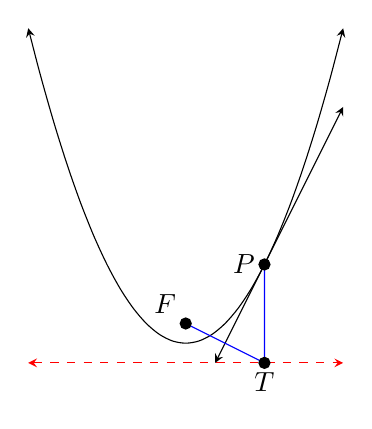
\begin{tikzpicture}[every node/.style={black}]
\draw[stealth-stealth] plot[smooth,domain=-2:2] (\x, {\x*\x});
\draw[stealth-stealth, dashed, red] (-2,-0.25) -- (2,-0.25);
\draw[stealth-stealth] (0.375,-0.25) -- (2,3);

\draw[blue] (1,1)--(1,-0.25) -- (0,0.25);

\filldraw (1,1) node[left] {$P$} circle (2pt);
\filldraw (1,-0.25) node[below] {$T$} circle (2pt);
\filldraw (0,0.25) node[above left] {$F$} circle (2pt);
\end{tikzpicture}
\end{center}

\subsubsection{Synthetic}
\begin{center}
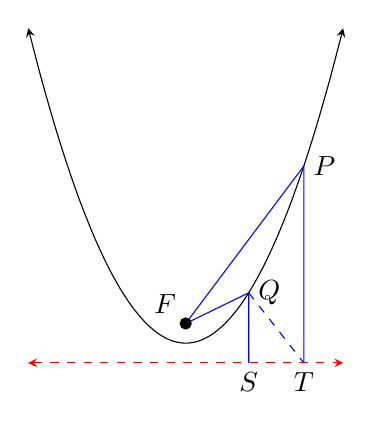
\begin{tikzpicture}[every node/.style={black}]
\draw[stealth-stealth] plot[smooth,domain=-2:2] (\x, {\x*\x});
\draw[stealth-stealth, dashed, red] (-2,-0.25) -- (2,-0.25);

\draw[blue] (0,0.25) -- (1.5,2.25) node[right] {$P$} -- (1.5,-0.25) node[below, black] {$T$};
\draw[blue] (0,0.25) -- (0.8,0.64) node[right] {$Q$} -- (0.8,-0.25) node[below, black] {$S$};
\draw[blue, dashed] (0.8,0.64) -- (1.5,-0.25);

\filldraw (0,0.25) node[above left] {$F$} circle (2pt);
\end{tikzpicture}
\end{center}
Let $F$ be the focus of the parabola,
let $P$ and $Q$ be distinct points on the parabola,
and let $T$ and $S$ be points of the directrix such that $PT$ and $QS$ are perpendicular to the directrix.
\\

By definition of a parabola $|QF|=|QS|$ and $|PF|=|PT|$,
and by construction $\triangle QST$ is a right angled triangle,
meaning:
\begin{equation*}
\begin{aligned}
|QT|^2 =& |QS|^2+|ST|^2 \\
=& |QF|^2+|ST|^2 \\
\Rightarrow |QT| >& |QF| \\
\end{aligned}
\end{equation*}

Hence the general point $Q$ isn't on the perpendicular bisector of $FT$,
but $P$ is, 
hence the perpendicular bisector of $FT$ is the tangent at $P$.

\subsubsection{Analytical}
Without loss of generality consider the unit parabola given by:
\[u: y=x^2\]
I state, without proof, that the focus is at $F=\left(0,\frac{1}{4}\right)$ and the directrix is given by:
\[d: y = -\frac{1}{4}\]
The tangent of $u$ at $P=(p,p^2)$ is given by:
\[t: y = 2px-p^2\]
Let $T=\left(p,-\frac{1}{4}\right)$ be the point of directrix such that $PT$ is perpendicular to it.
The line connecting the focus to $T$ is given by:
\[a: y= -\frac{x}{2p}+\frac{1}{4}\]
$a$ and $t$ are perpendicular since the product of their gradients is $-1$:
\[-\frac{1}{2p}\times 2p = -1\]
Also notice that the midpoint of $FT$ is given by:
\[M=\left(\frac{1}{2}(p+0),\frac{1}{2}\left(-\frac{1}{4}+\frac{1}{4}\right)\right) = \left(\frac{p}{2},0\right)\]
Is a point on both $a$ and $t$.

\subsection{Elementary Results}
\subsubsection{All points on a parabola are on the same side of the directrix as the focus:}
\begin{center}
\begin{tikzpicture}[every node/.style={black}]
	\draw[red,dashed,stealth-stealth] (-2.5,0) -- (2.5,0);
	\draw (-2,2) coordinate (F) node[above] {$F$} 
	-- (0,0) coordinate (Q) node[below] {$Q$} 
	-- (2,-2) coordinate (P) node[below] {$P$} 
	-- (2,0) coordinate (T) node[above] {$T$}
	pic[draw] {right angle = Q--T--P};
\end{tikzpicture}
\end{center}
Let $P$ be a point on the parabola on the opposite side of the focus $F$.
Let $T$ be a point on the directrix such that $PT$ is perpendicular to it.
Since $P$ and $F$ are on opposite sides of the directrix there is a point $Q$ where the segment $FP$ intersects the directrix.
\[|FP| > |QP| > |TP|\]
Which contradicts $|FP|=|TP|$,
hence $P$ doesn't exist.

\subsubsection{A line perpendicular to the directrix intersects a parabola at most once:}
\begin{center}
\begin{tikzpicture}[every node/.style={black}]
	\draw[red,dashed,stealth-stealth] (-2.5,0) -- (2.5,0);
	\coordinate (F) at (-1,3);
	\coordinate (P) at (1,4);
	\coordinate (Q) at (1,2);
	\coordinate (T) at (1,0);
	\coordinate (O) at (0,0);

	\draw (F) node[left] {$F$}
	-- (P) node[right] {$P$}
	-- (T) node[below] {$T$};

	\draw (F) -- (Q) node[right] {$Q$};

	\pic[draw] {right angle = Q--T--O};
\end{tikzpicture}
\end{center}
Let $T$ be the point where a perpendicular line to the directrix intersects the directrix.
Let $P$ and $Q$ be points on the same perpendicular line.
From the previous results both $P$ and $Q$ are on the same side as the focus $F$.
Without loss of generality let $P$ be the point further away from the directrix.
\\

Since $P$ and $Q$ are points on the parabola we have:
\[|FP| = |PT|\text{ and }|FQ| = |QT|\]
Substituting into the triangle inequality gives:
\begin{equation*}
\begin{aligned}
	|PT| =& |PQ|+|QT| \\
	=& |PQ| + |QF| \\
	>& |PF| \\
\end{aligned}
\end{equation*}
Which contradicts $|FP|=|TP|$,
hence distinct $P$ and $Q$ don't exist.

\subsubsection{A line perpendicular to the directrix intersects a parabola at least once:}
\begin{center}
\begin{tikzpicture}[every node/.style={black}]
	\draw[red,dashed,stealth-stealth] (-4.5,0) -- (2.5,0);
	\coordinate (F) at (-1,2);
	\coordinate (P) at (1,4);
	\coordinate (T) at (1,0);

	\draw (F) node[left] {$F$}
	-- (P) node[right] {$P$}
	-- (T) node[below] {$T$}
	-- (F);

	\pic[draw] {right angle = T--F--P};
\end{tikzpicture}
\end{center}
Let $F$ be the focus and let $T$ be a point on the directrix.
Extend a perpendicular line out from $T$, 
if the perpendicular intersects $F$ then the midpoint $M$ of $FT$ is on the parabola since:
\[|MF| = |MT|\]

If the perpendicular line doesn't go through $F$ suspend a second perpendicular line from the first perpendicular line at $F$ and let the two lines intersect at the point $P$.
\\

Let $X$ be a point on the segment $PT$ and define the function:
\[f(X) = |XF|-|XT|\]
We have:
\[f(T) = |TF|-|TT| > 0\]
and since $\angle PFT$ is a right angle we have $|PF| < |PT|$:
\[f(P) = |PF|-|PT| < |PT| -|PT| = 0\]
Hence by continuity there is a point $X_0$ in the segment $PT$ such that:
\[f(X_0) = 0\]
Meaning:
\[|X_0F| = |X_0T|\]
As required.

\subsubsection{A line perpendicular to the directrix intersects a parabola exactly once:}
Combine the last two results.

\subsubsection{Remarks}
These arguments are non-euclidean in two senses.
Neither sense as cool as "non-euclidean" sounds,
both of them still interesting.
\\

Firstly, is the use of continuity in the penultimate result.
The euclidean axioms famously don't include a concept of continuity.
Adding a continuity axiom to Euclid and when the concept is implicitly used has been an ongoing topic of research since the 19th century.
\\

Secondly, is the reverse.
Instead of using an another one,
we might not need to use all the euclidean axioms.
The first results don't use right-angles beyond showing $|PQ| > |PT|$ and the second result doesn't use them at all.
To me, this suggests that these results can be generalized to some subset of euclidean geometry.
I wasn't able to do so here,
but thoughts like this are why I wanted to think about parabolas more.

%% An unused diagram I don't feel like deleting.
%
%\begin{center}
%\begin{tikzpicture}[every node/.style={black}]
%	\coordinate (F) at (-2,0);
%	\coordinate (P) at (0,2);
%	\coordinate (Q) at (0,-2);
%	\coordinate (T) at (2,0);
%
%	\draw (F) node[left] {$F$} 
%	-- (P) node[above] {$P$}
%	-- (T) node[right] {$T$}
%	-- (Q) node[below] {$Q$}
%	-- (F);
%
%	\draw[red,dashed] (P) -- (Q);
%\end{tikzpicture}
%\end{center}
%With $P$ and $Q$ distinct points such that:
%\[|PT| = |PF| \text{ and } |QT| = |QF|\]
%This follows from the substitution into the triangle inequality:
%\[|PT| < |PQ|+|QT|\]
%Giving:
%\[|PT| < |PQ|+|QF|\]

%% An unused parts of an argument attempting to avoid right angles in the first result
%
%Let $F$ be the focus $P$ be the point $Q$ the intersection and $T$ the minimizing point on the directrix.
%
% Assume $|FQ| > |QT|$ then:
%\[|FP| \geq  |FQ|+|QP| > |QT|+|QP| > |TP|\]
%
%We also have:
%\[|FT|+|TP| > |FP| \geq |FQ|+|QP| = |TQ|+|QP| \geq |TP| \]

% Copyright 2023 Kieran W Harvie. All rights reserved.

\section{Time Evolution of a Two Dimensional Quantum System}
I was curious about the evolution of two dimensional quantum systems and decided to do a refresher. 
\\

Like all time-dependent problems start with the Schrödinger equation:
\[i\hbar \frac{\partial}{\partial t}\Psi = H\Psi\]
If $\Psi$ is an eigenvector of $H$ then we have:
\[i\hbar \frac{\partial}{\partial t}\Psi = E\Psi \Rightarrow \Psi = \exp(-i\hbar E t)\Psi_0\]
\\

A two-dimensional system where the energy levels are the same has a trivial evolution,
both gain phase at the same rate resulting in no observable change,
so assume there are two eigenvalues $\mu\pm\delta$.
\\

Let use working the orthonormal base of $H$ and define:
\[Z = \begin{bmatrix} 1&0\\0&-1\end{bmatrix},\quad E = \begin{bmatrix} \mu-\delta&0\\0&\mu+\delta\end{bmatrix}=\mu I -\delta Z\]
Then we have:
\[\Psi = \exp(-i\hbar E t)\Psi_0 = \exp(-i\hbar \mu t)\exp(i\hbar \delta Zt)\Psi_0\]
We will ignore the first factor as it's only relevant if working with a super system.

Consider the function $f(x) = \exp(i\hbar\delta t x)$ and apply the Cayley–Hamilton theorem to obtain:
\begin{equation*}
\begin{aligned}
\Psi =& \left(\exp(-i\hbar\delta t)\frac{Z+I}{2}-\exp(i\hbar\delta t)\frac{Z-I}{2}\right)\Psi_0 \\
=& \big[\cos(\hbar\delta t)I-i\sin(\hbar\delta t)Z\big]\Psi_0 \\
\end{aligned}
\end{equation*}
Observer that when $\delta t \rightarrow 0$ we have $\Psi \rightarrow \Psi_0$. 
This has two obvious sanity checks.
That as we return to the beginning, $t\rightarrow 0$, the state returns to $\Phi_0$ regardless of $\delta$.
And as the difference of the energy level shrinks, $\delta\rightarrow 0$, the state returns to $\Phi_0$ regardless of $t$.
\\

Other results include:

That for small $\delta$ we can keep the system in the $\Psi_0$ state for an inversely proportional time

That the system returns to $\Psi_0$ with a period of $\frac{\pi}{\hbar\delta}$.
Notice that the period is halved from the naïve value, 
as we only require the $\sin$ term to vanish.

\subsection{Change of Basis}
Assume the $\Psi_0$ isn't given in the orthonormal base of $H$.
Then we will need a change of basis matrix $P$ and have:
\[\Psi = P^{-1}\exp(-i\hbar E t)P\Psi_0\]
We can just substitute our worked expression for $\exp(-i\hbar Et)$ to give
\[\Psi = \big[\cos(\hbar\delta t)I-i\sin(\hbar\delta t)P^{-1}ZP\big]\Psi_0 \]
But lets pretend we didn't have the worked form,
what would we do?
\\

Well, interestingly we have:
\[P^{-1}\exp(-i\hbar E t)P\Psi_0= \exp(-P^{-1}i\hbar E tP)\Psi_0\]
So things don't change much yet.
And when it comes to applying the Cayley-Hamilton theorem we need the characteristic polynomials:
\begin{equation*}
\begin{aligned}
p_{P^{-1}MP}(x) =& \det(P^{-1}MP-xI) \\
=&\det(P^{-1}(M-xI)P) \\
=&\det(P^{-1})\det(M-xI)\det(P) \\
=&\det(M-xI) \\
\end{aligned}
\end{equation*}
Meaning the roots, eigenvalues, of one are the roots of another.
Meaning the result of Cayley-Hamilton is the same but with a different matrix subbed in.

From this point it's just algebra and left to the reader.
But what's interesting is that all the operations involved worked so well with:
\[M\mapsto P^{-1}MP\]
Which might be physically motivated.

In abstract algebra we would call this type of map a "conjugation", 
but that name already has a meaning in linear algebra,
so maybe "inner-automorphism" would be better.

% Copyright 2023 Kieran W Harvie. All rights reserved.

\section{Hermitian Operators}
This is some quick revision for something else.

For this section let $A$ and $B$ be hermitian operators in some complex vector space.
If they have them,
let $a$ be an eigenvector of $A$ with value $\alpha$.
Likewise for $b$ and $\beta$ for $B$.

\subsection{Immediate Results}
\subsubsection{Theorem: All eigenvalues are real}
\begin{equation*}
\begin{aligned}
\alpha\langle a,a\rangle =& \langle a,\alpha a\rangle\\
	=& \langle a, Aa\rangle\\
	=& \langle Aa, a\rangle\\
	=& \bar{\alpha}\langle a,a\rangle
\end{aligned}
\end{equation*}
Since eigenvectors can't be zero we require $\alpha=\bar{\alpha}$.

\subsubsection{Theorem: $\ker A = \img A^\perp$}
Assume $Ax=0$ and let $y$ be any arbitrary vector,
then:
\[0 = \langle Ax,y\rangle = \langle x, Ay\rangle \]
Hence $x\in\img A^\perp$

\subsection{Finite, Nonzero, Complex Vector Space}
For this section we assume that $A$ and $B$ belong to a finite, nonzero, complex vector space.
\\

A discussion on all these constraints will likely be included at the end.
But the reason of the constraints is the following powerful theorem:
\subsubsection{Theorem: If $A$ is a linear operator on a finite, nonzero, complex vector space then there exits at least one unit eigenvector.}
By the fundamental theorem of algebra the characteristic polynomial of $A$ has at least one solution and hence $A$ has at least one eigenvector.

Without loss of generality we can rescale the eigenvector to make it a unit vector.

\subsubsection{Remark:}
This existence theorem is very powerful and but uses all of the conditions.
Finite to get a polynomial, nonzero so it's not a constant polynomial, complex to make that polynomial have a root.

\subsubsection{Corollary: Let $A$ be the transform of a nonzero invariant subspace $V$, then $V$ includes a unit eigenvector of $A$:}
$V$ inherits finiteness and complex from its super space,
we can also treat $A$ as a linear operator on $V$ by invariance,
and since $V$ is also assumed to be nonzero the previous theorem applies.

\subsubsection{Lemma: Let $E$ be a set of eigenvectors for $A$ then $A$ preserves $\spn(E)^\perp$:}
If $x\in\spn{E}^\perp$ then for all $c_n$ we have:
\begin{equation*}
\begin{aligned}
	\langle Ax, \sum_n c_na_n\rangle =& \langle x, A\sum_n c_na_n\rangle\\
	=& \langle x, \sum_n c_n\alpha_na_n\rangle\\
	=&0 \\
\end{aligned}
\end{equation*}

\subsubsection{Theorem: There exits an orthonormal basis of eigenvectors of $A$}
From the existence theorem there exits a unit eigenvector $a_0$.
Let $S_0 = \spn({a_0})^\perp$, then by the previous lemma $S_0$ is an invariant subspace.
Hence by the existence theorem there is a unit eigenvector $a_1\in S_0$.
Likewise define $S_1 = \spn(\{a_0,a_1\})^\perp$ and so on until we get a basis.

\subsubsection{Theorem: If $A$ and $B$ commute then there exits a mutuality orthogonal eigenvectors basis}
From the existence theorem there is an eigenvector $a$ of $A$.
Define the set:
\[W = \spn(\{B^na\,|\,n\in\mathbb{N}\})\]
Let $w\in W$, then by definition we have $Bw\in W$ hence by the existence corollary there exits unit eigenvector vector $w$ of $B$ in $W$.
From commutativity and the definition of $W$ we also have $Aw=aw$.
Hence $w$ is an eigenvector of both operations.
We can build up a basis with induction,
like the previous theorem.

\subsection{All Those Conditions}
The critical points in the previous proofs was the existence theorem and induction on the eigenvectors.
But the existence theorem didn't use the fact the operators where Hermitian,
so surely we can remove some of those conditions!

Well we could weaken Complex to algebraically closed field without hermitian but we can't remove finite and nonzero.
The nonzero condition isn't much of a concern, 
the vector field $\{0\}$ isn't interesting but to see why we can't remove finite consider the set of square-integrable functions on $[0,1]$.
\\

The operator $[Af](t) \mapsto tf(t)$ is clearly Hermitian because the integrating veritable is real:
\[
	\langle f,tg\rangle = \int_0^1\overline{g(t)}tf(t)\,dt = \int_0^1\overline{tg(t)}f(t)\,dt = \langle tf,g\rangle
\]
But has no eigenvector as:
\[tf(t)=\alpha f(t)\]
Means $f(t)$ can only be nonzero at $t=\alpha$,
which means only $f(\alpha)$ can be nonzero.
Remembering that the vector space only cares about functions up to the equivalence class of being equal "almost everywhere" this function is the constant $0$ function.
\\

This operator is clearly important for functional analysis,
so we can't define a set of nicer functions,
so what do we do?
There is one interesting result:
\\

There exits a number $\lambda$ equal to $||A||$ or $-||A||$ and a sequence of unitary vectors $x_n$ such that:
\[\lim_{n\rightarrow\infty}\big(Ax_n-\lambda x_n\big) = 0\]
Which is like $\lambda$ being an eigenvalue in the limit.
\\

Applying this eigen-limit idea to square integral functions and we get the $\delta(t-\alpha)$ functions,
which can be approached by many different sequence of limit functions.

% Copyright 2023 Kieran W Harvie. All rights reserved.
% Don't like the order things are presented, but not enough to change it.

\section{Hadamard Matrix}
I came across this cute set of matrices today:
\[H_{2^k} = \begin{bmatrix} 1&1\\1&-1\end{bmatrix}\otimes H_{2^{k-1}},\quad H_{2} = \begin{bmatrix} 1&1\\1&-1\end{bmatrix}\]
They are called the Hadamard matrices and their first interesting property is that their columns are orthogonal.
\\

To see this consider two matrices $A$ and $B$, we have:
\[(AB^T)_{i,j} = \sum_{k=1}^nA_{i,k}B_{j,k}\]
Which is the dot product of the $i^\text{th}$ and $j^\text{th}$ columns of $A$ and $B$.
Hence $H_n$'s columns being orthogonal is the same as:
\[(H_nH_n^T)_{i,j} = f(i)\delta_{i,j}\]

For induction assume:
\[H_{2^{k-1}}H_{2^{k-1}}^T=2^{k-1}I_{2^{k-1}}\]
Hence:
\begin{equation*}
\begin{aligned}
	H_{2^k}H_{2^k}^T =& \begin{bmatrix} H_{2^{k-1}}&H_{2^{k-1}}\\H_{2^{k-1}}&-H_{2^{k-1}}\end{bmatrix}
	\begin{bmatrix} H_{2^{k-1}}^T&H_{2^{k-1}}^T\\H_{2^{k-1}}^T&-H_{2^{k-1}}^T\end{bmatrix}\\
	=&\begin{bmatrix} 2H_{2^{k-1}}H_{2^{k-1}}^T&H_{2^{k-1}}H_{2^{k-1}}^T-H_{2^{k-1}}H_{2^{k-1}}^T\\
	H_{2^{k-1}}H_{2^{k-1}}^T-H_{2^{k-1}}H_{2^{k-1}}^T&2H_{2^{k-1}}H_{2^{k-1}}^T\\\end{bmatrix}\\
	=&\begin{bmatrix}2^kI_{2^{k-1}}&0\\0&2^kI_{2^{k-1}}\end{bmatrix} \\
	=&2^kI_{2^k} \\
\end{aligned}
\end{equation*}
Which shows $H_n$'s columns are orthogonal,
and also that:
\[H_n^{-1} = \frac{1}{2^n}H_n^T\]

Taking the determinates of both sides:
\[\det(H_n)^2=\det(nI_n) = n^n\]
Hence:
\[|\det(H_n)|=  n^\frac{n}{2}\]
And it actually turn out that all other $n\times n$ real matrices with elements of magnitude less then or equal to one have a determinate whose magnitude is less than this, which is pretty cool.

% This method sucked and I abandoned it, even though it's closer to my minds eye.
%
% \[\left(H_{2^k}\right)_{i,j} = \begin{cases} 
% (H_{2^{k-1}})_{i,j} & i\leq 2^{k-1} \text{ and } j\leq 2^{k-1}\\
% (H_{2^{k-1}})_{i-2^{k-1},j} & i> 2^{k-1} \text{ and } j\leq 2^{k-1}\\
% (H_{2^{k-1}})_{i,j-2^{k-1}} & i\leq 2^{k-1} \text{ and } j> 2^{k-1}\\
% -(H_{2^{k-1}})_{i-2^{k-1},j-2^{k-1}} & i> 2^{k-1} \text{ and } j> 2^{k-1}\\
% \end{cases}\]
% \begin{equation*}
% \begin{aligned}
% (H_{2^k}H_{2^k}^T)_{i,j} =& \sum_{k=1}^{2^k}(H_{2^k})_{i,k}(H_{2^k})_{j,k} \\
% =& \sum_{k=1}^{2^{k-1}}(H_{2^k})_{i,k}(H_{2^k})_{j,k} + \sum_{k=2^{k-1}+1}^{2^k}(H_{2^k})_{i,k}(H_{2^k})_{j,k} \\
% \end{aligned}
% \end{equation*}

% Copyright 2023 Kieran W Harvie. All rights reserved.

\section{Information Theory based Entropy}
I want to do some entropy/temperature calculations only using motivations from a information perspective.
We will start with the classic problem:
\begin{equation*}
\begin{aligned}
	\text{Maximize: }& H=-\sum_i p_i\ln(p_i)\\
	\text{Subject to: }& \sum_ip_i=1,\quad \sum_ip_iw_i = \mu \\
\end{aligned}
\end{equation*}
Start with a standard Lagrangian:
\[ L = -\sum_ip_i\ln(p_i)+a\left(\sum_i p_i - 1\right) + b\left(\sum_i p_iw_i - \mu\right)\]
Giving:
\[p_i = \exp(-1-a-bw_i)\]
We can easily remove $a$ by normalizing:
\[p_i = \frac{1}{Z(b)}\exp(-bw_i)\]
Where:
\[Z(t) = \sum_i \exp(-tw_i)\]
Likewise for $\mu$:
\[\mu = \sum_ip_iw_i = \frac{1}{Z(b)}\sum_iw_i\exp(-bw_i)\]
Substituting back into $H$:
\begin{equation*}
\begin{aligned}
	H =& \frac{1}{Z(b)}\sum_i\bigg(\exp(-bw_i)(bw_i+\ln(Z(b))\bigg)\\
	=& \frac{1}{Z(b)}\bigg(bZ(b)\mu+Z(b)\ln(Z(b))\bigg)\\
	=& b\mu+\ln(Z(b))\\
\end{aligned}
\end{equation*}

The $b\mu$ term already lets us interpret $b^{-1}$ as acting like temperature.
As we'd expect an increase of $\mu$ to allows us to increase entropy because it allows us to distribute more probability to larger $w_i$.
\\

Let go further by noticing that:
\[\mu = - \frac{Z'(b)}{Z(b)} = -\frac{d}{d\,b}\ln(Z(b))\]

This lets us formalizes the statement "more probability going to larger $w_i$" from earlier.
\begin{equation*}
\begin{aligned}
	\frac{d p_i}{d \mu} =& \left(\frac{-w_i}{Z(b)}\exp(-bw_i)-\frac{Z'(b)}{Z^2(b)}\exp(-bw_i)\right)\frac{d\,b}{d\,\mu}\\
	=&p_i(\mu-w_i)\frac{d\,b}{d\,\mu}\\
\end{aligned}
\end{equation*}

And also:
\[\frac{d\,H}{d\,b} = b\frac{d\,\mu}{d\,b}+\mu+\frac{Z'(b)}{Z(b)} = b\frac{d\,\mu}{d\,b}+\mu -\mu =b\frac{d\,\mu}{d\,b}\]
Which gives:
\[\frac{d\, H}{d\, \mu} = b\]
As expected.

% Copyright 2023 Kieran W Harvie. All rights reserved.

\section{Legendre Transform}
I've used the Legendre transform a lot and always understood that it transformed between conjugate variables but never understood the motivation of its formal definition. 
Well I've thought of a good motivated argument.
\\

Let $f$ be a strictly convex differentiable function in $x$.
Then $\frac{\partial f}{\partial x}$ is a strictly increasing function.
This means $\frac{\partial f}{\partial x}$ is injective and we can defined a function $g$ such that:
\[g\left(\frac{\partial f}{\partial x}\bigg|_{x_0}\right) = x_0\]
And we can further define a new function $f^*$,
up to an additive constant,
such that:
\[\frac{\partial f^*}{\partial p} = g(p)\]
This is the Legendre Transform.
\\

This transforms usefulness comes from looking at the functions differential.
Let $f(x,y)$ and consider a point $(x_0,y_0)$ where:
\[\frac{\partial f}{\partial x}\bigg|_{(x_0,y_0)} = p,\quad\frac{\partial f}{\partial y}\bigg|_{(x_0,y_0)} = v \]
Giving the differential:
\[df = pdx+vdy\]
Now consider a $f^*(p,y)$ where $f^*$'s first argument is Legendre transformed from $f$'s, 
and the second is unchanged.
This gives:
\[df^* = xdp+vdy\]
You can see that the coefficient and differential of the first term has swapped,
pretty useful.
\\

This argument seems more motivated to me, 
but the domain of the transform can be widened to merely require $f$ being convex on $D$ by defining:
\[f^*(p) = \sup_{x\in D}\big[px-f(x)\big]\]
To see that this definition extends the strictly convex differentiable case derive the inner function by $x$ and set to zero:
\[p-f'(x)=0\]
But $f$ is injective,
so we can defined $g$ as before and obtain:
\[f'(g(p)) = p\]
meaning the maximal value of $x$ is $g(p)$, 
giving:
\[f^*(p) = pg(p)-f(g(p))\]
Deriving by $p$ gives:
% f^*'(p) doesn't work, don't feel like fixing
\[\frac{d}{d p}f^*(p) = g(p)+pg'(p)-g'(p)f'(g(p))\]
Substituting in $f'(g(p)) = p$ gives:
\[\frac{d}{d p}f^*(p) = g(p)+pg'(p)-g'(p)p = g(p)\]
As expected.

% Copyright 2023 Kieran W Harvie. All rights reserved.

\section{Weierstrass-Erdmann Corner Conditions}
I saw an enlightening Calculus of Variation problem that involved some of the more interesting results from the field.

Find $x(t)$ such that:
\[I=\int_0^2(1-\dot{x})^2\dot{x}^2\,dt\]
Is minimized with endpoints $x(0)=0$ and $x(2)=1$.
\\

By inspection $F(t,x,\dot{x})=(1-\dot{x})^2\dot{x}^2\geq 0$ making $I\geq 0$ with the $F$ vanishing iff $\dot{x} = 0,1$.
Hence any piecewise combinations of lines with gradients $0$ or $1$ from $(0,0)$ to $(2,1)$ works.
For example,
the solution of a straight line from $(0,0)$ to $(1,1)$ then to $(2,1)$ is a minimum.
This solution is continuous but not differentiable.

Now lets use more standard methods.
First calculate a table of useful properties of $F$:
\begin{equation*}
\begin{aligned}
	F_x =& 0 \\
	F_{\dot{x}} =& 2\dot{x}(1-\dot{x})(1-2\dot{x})\\
	F_{\dot{x}^2} =& 12\dot{x}^2-12\dot{x}+2\\
	\frac{d}{d\,t}F_{\dot{x}} =& \ddot{x}F_{\dot{x}^2} \\
	=& \ddot{x}(12\dot{x}^2-12\dot{x}+2)\\
\end{aligned}
\end{equation*}

The Euler-Lagrange equation,
combined with the first and last line,
means that all extremals take the form:
\[x(t) = at+b\]
These are lines, 
but a line directly between the endpoints is:
\[x(t) = \frac{1}{2}t\]
Meaning:
\[F= \frac{1}{16}>0\]

This is clearly greater than the piecewise solutions,
but lets pretend we don't know that and use some other results. 
\\

\subsection{Only solution is not a Minimum}
The Legendre-Clebsch condition says that in order for $x_0(t)$ to minimize $\int_U F(t,x,\dot{x})\,dt$ we require:
\[ t\in U \Rightarrow F_{\dot{x}^2}(t,x_0,\dot{x_0}) \geq 0\]
But we have:
\[x(t)=\frac{1}{2}t \Rightarrow F_{\dot{x}^2} = -1\]
Meaning the only solution of the Euler-Lagrange equation isn't a minimum.
Does that mean there are none?
No, just none in the set of functions that match the Euler-Lagrange equations assumptions.
(At least continuously differentiable, but the set may be bigger).
But clearly minimal solutions exits from the beginning.

\subsection{Corners} 
Continue to pretend we don't know the piecewise solutions.
The Weierstrass-Erdmann corner condition states that for first-order derivate discontinuities,
or "corners", 
at $t_0$ the functions on either side,
$x_0$ and $x_1$ must satisfy:
\[F_{\dot{x}}(t_0,x_0,\dot{x_0}) = F_{\dot{x}}(t_0,x_1,\dot{x_1})\]
and
\[F_{\dot{x}}(t_0,x_0,\dot{x_0})\dot{x_0}(t_0)-F(t_0,x_0,\dot{x_0}) = F_{\dot{x}}(t_0,x_1,\dot{x_1})\dot{x_1}(t_0)-F(t_0,x_1,\dot{x_1})\]

Our $F$ is pretty simple, 
only put a restrictions on $\dot{x_n}$, 
\begin{equation*}
\begin{aligned}
	\dot{x_0}(1-\dot{x_0})(1-2\dot{x_0}) =& \dot{x_1}(1-\dot{x_1})(1-2\dot{x_1}) \\
	\dot{x_0}^2(1-\dot{x_0})(1-3\dot{x_0}) =& \dot{x_1}^2(1-\dot{x_1})(1-3\dot{x_1}) \\
\end{aligned}
\end{equation*}
This means $\dot{x_0},\dot{x_1}\in\{0,1\}$.
It's hard to see this from algebra alone,
or maybe it's just that I'm tired,
but plotting $x(1-x)(1-2x)$ and $x^2(1-x)(1-3x)$ shows it pretty well.
\\

Observe that this is just the piecewise solutions we got from first inspection.
Pretty cool.

\subsection{Next Steps}
There were other goodies in the place I found this problem.

First there are some notes here for implicit boundaries:
\[S(x,y)=0\]
Which might be useful for shader stuff,
but haven't pieced it together yet.
\\

There is also an iterative method of solving Calculus of Variation problems.
It might be interesting to inspect this iteration and see the differential solutions converge to the piecewise solutions.
Or maybe something else cooler!!

% Copyright 2023-2024 Kieran W Harvie. All rights reserved.

\section{Rational Residue}
\label{showcase:rational_residue}
I saw a cool result,
that if $P$ and $Q$ are polynomials and $Q$ has a first order root at $a$ then the then:
\[\Res\left(\frac{P}{Q},a\right) = \frac{P(a)}{Q'(a)} \]
Which can save a lot of time over factorizing, 
which is what I would have done in the past.
\\

This trick follows directly from:
\[Q'(a)=\frac{d}{dz}(z-a)q(z)\bigg|_a = q(a)\]
and
\[\oint_\gamma\frac{P(z)}{Q(z)}\,dz = \oint_\gamma \frac{P(z)}{(z-a)q(z)}\,dz = 2\pi i\frac{P(a)}{q(a)}\]
\\

I thought this might be generalizable since the general Leibniz rule on $Q(z)=(z-a)^2q(z)$ gives:
\[Q''(a)=2q(a),\quad Q'''(a)=6q'(a)\]
Hence for a second order root:
\begin{equation*}
\begin{aligned}
	\oint_\gamma\frac{P(z)}{Q(z)}\,dz =& \oint_\gamma \frac{P(z)}{(z-a)^2q(z)}\,dz \\
	=& \pi i\frac{P'(a)q(a)-P(a)q'(a)}{q(a)^2}\\
	=& 2\pi i\frac{3P'(a)Q''(a)-P(a)Q'''(a)}{3Q'(a)^2}\\
\end{aligned}
\end{equation*}
Giving:
\[\Res\left(\frac{P}{Q},a\right)= \frac{3P'(a)Q''(a)-P(a)Q'''(a)}{3Q'(a)^2} \]

Which isn't as cool as the first order case,
and I don't feel like dealing with higher derivatives.
Still cool though.

\subsection{Actual closed form}
There actually is a way to get a closed form without dealing with higher order derivatives of reciprocals.
The idea is to use the Bézout trick to get a polynomial that acts like a reciprocal at $z=a$.
\\

Let $Q$ be a polynomial with an $n$ ordered root at $a$.
Then define $q$ as:
\[Q(z) = (z-a)^nq(z)\]
Since $\gcd(q(z),(z-a)^n) = 1$ from the Bézout's identity, there exits polynomials $r$ and $s$ such that:
\[r(z)(z-a)^n+s(z)q(z)=1\]
Hence:
\[\frac{P(z)}{(z-a)^nq(z)}(1-s(z)q(z)) = \frac{P(z)}{q(z)}r(z)\]
Has no poles at $a$ and vanishes in the contour integral.
Meaning we can split up its terms to give:
\[\oint_\gamma\frac{P(z)}{(z-a)^nq(z)}\,dz = \oint_\gamma \frac{P(z)s(z)}{(z-a)^n}\,dz\]
Resulting in the clean:
\[\Res\left(\frac{P}{Q},a\right) = \frac{1}{(n-1)!}\frac{d^{n-1}}{dz^{n-1}}P(z)s(z)\bigg|_{z=a}\]

\subsubsection{Remarks}
You can use use the standard extended Euclid algorithm to calculate $s$ from $q$, or $q$ from $s$.
But the relation:
\[r(z)(z-a)^n+s(z)q(z)=1\]
Can be derived $n-1$ times and set $z=a$ to get a linear system between derivatives of $s$ and $q$.
So why bother with Bézout at all?
Well you would need to prove that the coefficients from the system converge to an analytic function,
Bézout side steps this.
\\

I'm also wondering about $s^{(n)}(a)=0$,
because we loose information about $F$ in the sum when this happens.
Also working backwards, can we have any $s$.
Not $s(z) = z-a$ obviously, but we can add another power to keep it? 
$s(z) = z^2+z-a$?

\subsection{A Generalization}
Generate new solutions to the Bézout Identity in the standard way:
\[[r(z)-h(z)s(z)](z-a)^n+s(z)[q(z)+(z-a)^nh(z)]=1\]
If we choose $h$ such that $r(z)-h(z)s(z)$ is holomorphic,
easy since $r$ and $s$ are polynomials, we have, given $\gamma$ is small enough to not add new poles from $h$:
\[\oint_\gamma\frac{P(z)}{(z-a)^n[q(z)+(z-a)^nh(z)]}\,dz = \oint_\gamma \frac{P(z)s(z)}{(z-a)^n}\,dz= \frac{1}{(n-1)!}\frac{d^{n-1}}{dz^{n-1}}P(z)s(z)\bigg|_{z=a}\]

Observe that all function $q'(z)$ such $(z-a)^n | q(z)-q'(z)$ can be written as $q'(z) = q(z)+(z-a)^nh(z)$ for some holomorphic $h$ giving the pretty cool result that only the fist $n$ derivatives of $q'$ effect the value of the contour integral.
(Also observe that $r'(z) = r(z)-h(z)s(z)$ means $r'$ agrees  with $r$ on $s$ helping motivate the LHS)
\\

$q'(z)=1$ gives $s(z)=1-(z-a)^n,\,r'(z)=1$ and hence Cauchy's integral formula and hence generalizes it.

This could also  be used to extract terms from the reciprocal of a generating function.

% Copyright 2023 Kieran W Harvie. All rights reserved.

\section{Summation by Parts}
During a boring meeting I was reminded of a cool trick called "Summation by Parts".
Given two sequences $a_n$ and $b_n$ define $B_n = \sum_{k=0}^nb_n$.
Then we have:
\[\sum_{k=0}^Na_nb_n = a_NB_N-\sum_{n=0}^{N-1}B_n(a_{n+1}-a_n)\]
The name is clearly in reference to it being the discrete counterpart to integration by parts.
With integration replaced with summation and derivatives with difference.
\\

I will not be proving this formula, 
doing so is simple algebra.

\subsection{Nicomachus's Theorem}
Nicomachus's Theorem is the name of the following identity:
\[\sum_{k=1}^nk^3 = \left(\sum_{k=1}^nk\right)^2\]
It's a common object of recreational math and visual proofs in particular.
And while I proofs of it have reached the point of annoyance,
visual ones in particular,
Summation of Parts provides another proof that motivates the squaring.
\\

Let $\sigma_n = \sum_{k=0}^nk$ and set $a_n = \sigma_n$ and $b_n=n$.
Hence $B_n = \sigma_n$ and $a_{n+1}-a_n = n+1$ giving:
\[\sum_{k=0}^Nn\sigma_n = \sigma_n^2-\sum_{n=0}^{N-1}(n+1)\sigma_n\]
Since $\sigma_0=0$ we can shift the LHS sum up one to match the RHS's bound:
\[\sum_{k=0}^Nn\sigma_n = \sigma_n^2-\sum_{n=0}^{N}n\sigma_{n-1}\]
Giving:
\[\sum_{k=0}^Nn(\sigma_n+\sigma_{n-1}) = \sigma_n^2\]
The observation that $\sigma_n+\sigma_{n-1}=n^2$ completes the proof.
\\

It's worth nothing this proof doesn't require an explicit closed formula for $\sigma_n$.
Instead only needing $\sigma_{n+1}-\sigma_n = n+1$,$\sigma_{n+1}+\sigma_n =(n+1)^2$ and $\sigma_0 = 0$.
Yes, a close form follows easily from these properties as:
\[\sigma_{n+1} = \frac{1}{2}((\sigma_{n+1}+\sigma_n)+(\sigma_{n+1}-\sigma_n))\]
But it's still a cool proof

\subsection{Continuous Summation by Parts}
Consider the case here $a_n$ is given by a continuously differential function $a(x)$, 
that is $a_n = a(n)$.
Likewise modify $B_n$ into a continuous function,
$B(x) = B_{\lfloor x \rfloor}$.
Hence we can write the RHS summation as:
\begin{equation*}
\begin{aligned}
	\sum_{n=0}^{N-1}B_n(a_{n+1}-a_n) =& \sum_{n=0}^{N-1}B(n)(a(n+1)-a(n))\\
	=& \sum_{n=0}^{N-1}B(n)\int_n^{n+1}a'(t)\,dt\\
\end{aligned}
\end{equation*}
Note that $B(t)$ is constant for $t\in(n,n+1)$ allowing us to move it into the integral:
\begin{equation*}
\begin{aligned}
	\sum_{n=0}^{N-1}B_n(a_{n+1}-a_n) =& \sum_{n=0}^{N-1}\int_n^{n+1}B(t)a'(t)\,dt\\
	=& \int_0^{n}B(t)a'(t)\,dt\\
\end{aligned}
\end{equation*}

Substitution into the original equation gives:
\[\sum_{k=0}^Na_nb_n = a_NB_N-\int_0^{n}B(t)a'(t)\,dt\]
If we cancel the fractional parts of the product and integral on the RHS we get the more general:
\[\sum_{0\leq n\leq x}a_nb_n = a(x)B(x)-\int_0^{x}B(t)a'(t)\,dt\]

This isn't a particularly good formula for relating a sum to an integral,
see the Euler-Maclaurin formula,
but it's still good enough for some results:

\subsubsection{Results:}
Let $a(x)=\ln(x)$ and $b_n=1$ then we have:
\[\sum_{1\leq n\leq x}\ln(n) = \lfloor x \rfloor \ln(x)-\int_1^xt\,\frac{1}{t}\,dt = x\ln(x) - x +O(\ln(x))\]

Let $a(x)=\frac{1}{x}$ and $b_n =1$
\[\sum_{1\leq n\leq x}\frac{1}{n} = \frac{\lfloor x \rfloor}{x}-\int_1^xt\,\frac{-1}{t^2}\,dt = \ln(x) +O(1)\]

Both of these bounds are useful for computer science. 

% Copyright 2023 Kieran W Harvie. All rights reserved.

\section{Bounds of Three Series}
Even though I'm sick I found an interesting problem on the internet.
Given positive $a_1,b_1,c_1>0$ and:
\begin{equation*}
\begin{aligned}
	a_{n+1} =& b_n+\frac{1}{c_n}\\
	b_{n+1} =& c_n+\frac{1}{a_n}\\
	c_{n+1} =& a_n+\frac{1}{b_n}\\
\end{aligned}
\end{equation*}

Show that at least one of $a_{800},b_{800},c_{800}$ is greater than 40 and that all sequences are unbounded.

\subsection{Lemma: Closed form for $x_{n+1} = x_n+\frac{k}{x_n}$} 
The closed form is this:
\[ x_{n+1}^2 = x_1^2+2nk+k^2\sum_{l=1}^n\frac{1}{x_l^2}\]
This result is nothing special, 
just a lot of algebra,
the plan is to first get a result for the product of successive terms,
then get perform induction on the product,
and finally cleanup to get the final form.

\begin{equation*}
\begin{aligned}
	x_{n+2}x_{n+1} =& \left(x_{n+1}+\frac{k}{x_{n+1}}\right)x_{n+1}\\
	=& \left(x_n+\frac{k}{x_n}+\frac{k}{x_{n+1}}\right)x_{n+1}\\
	=& x_{n+1}x_n + k +k\frac{x_{n+1}}{x_n} \\
	=& x_{n+1}x_n + k +k\frac{1}{x_n}\left(x_n+\frac{k}{x_n}\right) \\
	=& x_{n+1}x_n + 2k +\frac{k^2}{x_n^2} \\
\end{aligned}
\end{equation*}

Induction gives:
\[ x_{n+2}x_{n+1} = x_2x_1+2nk+k^2\sum_{l=1}^n\frac{1}{x_l^2}\]

Then you clean up by using the initial relation on $x_{n+2}$ and $x_2$.

\subsection{Unbounded:}
Let $s_n = a_n+b_n+c_n$, 
from the HM-AM inequality we have:
\[\frac{1}{a_n}+\frac{1}{b_n}+\frac{1}{c_n} \geq \frac{9}{s_n}\]
With equality if and only if $a_n=b_n=c_n$.
\\

From the series definition we have:
\[s_{n+1} = s_n + \frac{1}{a_n}+\frac{1}{b_n}+\frac{1}{c_n} \geq s_n+\frac{9}{s_n}\]

Since $a_n=b_n=c_n \Rightarrow a_{n+1}=b_{n+1}=c_{n+1}$ we have $s_n$ is bounded by:
\[ s_{n+1}^2 \geq s_1^2+18n+81\sum_{l=1}^n\frac{1}{s_l^2}\]
Hence $s_n$ grows at least as much as $3\sqrt{2n}$,
which is unbounded.
\\

If the sum is unbounded at least one of the series is unbounded.
And if at least one series is unbounded the "swapping" nature of the series means that they all are.

\subsection{$800^\text{th}$ terms:}
Consider the bound sum:
\[ s_{n+1}^2 \geq s_1^2+18n+81\sum_{l=1}^n\frac{1}{s_l^2}\]
If $s_n \leq 1$ then $s_{n+1} > 1$ hence at least half of the time $\frac{1}{s_l^2}$ must be greater than one.
Giving the new bound:
\[ s_{n+1}^2 > 18n+81\left\lfloor\frac{n}{2}\right\rfloor\]
(This isn't a particularly good bound, we could consider $s_1$ separately, but if works the result we need)
Substituting in $n=799$ gives:
\[s_{800}^2 > 18\times799+81\times398 > 18\times800 = 3^2\times40^2\]
Hence:
\[a_{800}+b_{800}+c_{800} = s_{800} > 3\times40\]
From pigeon holing at least one LHS term is greater than 40.

\subsection{Remarks}
This is yet another example of this Olympian style problem where I had to be prompted to consider the HM-AM inequality.

Although I was working with inequalities between elementary polynomial sums so wasn't that far away myself,
and the other advice that was given was just straight up wrong, 
so I should probably just remember to use the inequality means in the future and let it go.

% Copyright 2023-2024 Kieran W Harvie. All rights reserved.

\section{Simplicial Homology}
I need to revise Simplicial Homology so I'm going to give some definitions and then work some examples.

\subsection{Simplicial Definitions}

\subsubsection{Simplex:}
A simplex is a generalization of a triangle to higher/lower dimensions:

\begin{itemize}
	\item 0-simplex is a point
	\item 1-simplex is a segment
	\item 2-simplex is a triangle
	\item 3-simplex is a tetrahedron
\end{itemize}

For our purposes we specify a simplex with an ordered word written from the set of points.
For example $a$ is a point, $bc$ is a segment, and $abc$ is a triangle:
\begin{center}
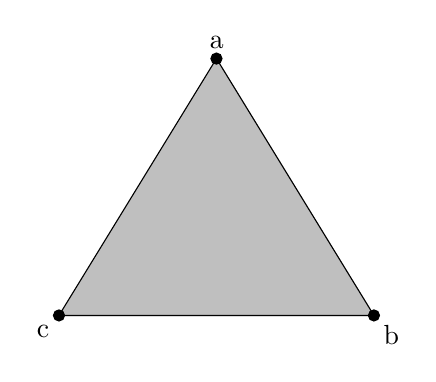
\begin{tikzpicture}
	\filldraw[lightgray] (-2,0)  --(2,0)--(0,3.26210161512);
	\draw (-2,0)--(2,0)--(0,3.26210161512)--(-2,0);
	\filldraw (-2,0) node[below left] {c} circle (2pt);
	\filldraw (2,0) node[below right] {b} circle (2pt);
	\filldraw (0,3.26210161512) node[above] {a} circle (2pt);
\end{tikzpicture}
\end{center}
Two important remarks.
Firstly, $abc\neq acb$ the former one goes around counter-clockwise and the later clockwise.
Secondly, the set $\{ab,bc,bc\}$ is not a triangle and is not the same as $abc$ or $\{abc\}$.
It's all the edges of a triangle but not its interior.

\subsubsection{Face:}
$n$ 0-simplexes defines a $n$-simplex and is called the face of the points.
Conversely the vertices that define a simplex and all the faces that come from that simplex are called the faces of the original simplex.

\subsubsection{Geometric Simplicial Complex}
A Geometric Simplicial Complex $\mathcal{K}$ is a set of simplexes such that:
\begin{enumerate}
	\item Every face of an element of $\mathcal{K}$ is also an element of $\mathcal{K}$.
	\item The non-empty intersection of two simplexes $\sigma_0,\,\sigma_1\in\mathcal{K}$ is a face of both $\sigma_1$ and $\sigma_0$.
\end{enumerate}

\subsubsection{Chain}
A $k$-chain of $\mathcal{K}$ is a formal linear sum of $k$-simplexes.
A $2$-chain is naturally interpreted as a,
possible disconnected and repeated, 
path through $\mathcal{K}$.
\\

More formally, 
given a complex $\mathcal{K}$ the group of $n$-chain $C_n(\mathcal{K})$ is a free $\mathbb{Z}$-module over the $n$-simplexes where two simplexes are equal if they have the same orientation\footnote{The words are even permutation of each other.} and additive inverse if opposite.
(Define $C_{-1} = 0$ for convenience).
\\

For example: $ab+bc$ is the path from $a$ to $c$ through $b$,
$abc = -acb$ are the same triangle with different handedness,
$2ab+dc$ is going over $ab$ twice then jumping to $dc$.
\\

Although the lower dimensions have intuitive geometric interpretation the whole configuration can more intuitively viewed as a combinatoric exercise. 

\subsection{Homology Definitions}
\subsubsection{Boundary Operator}
Given a simplex $\sigma$ define $\sigma_k$ as the same word a $\sigma$ with the $k^\text{th}$ point removed.
The boundary operator $\partial_k:C_k\rightarrow C_{k-1}$ is defined as:
\[\partial_k(\sigma) = \sum_{i=0}^k(-1)^i\sigma_i\]
The boundary of a $0$-simplex is $0$,
the boundary of a $1$-simplex is final point minus inital,
the boundary of a $2$-simplex is it's normal boundary (hence the name).
\\

\begin{equation*}
\begin{aligned}
	\partial_0(a) &= 0\\
	\partial_1(ab) &= b-a\\
	\partial_2(abc) &= ac + cb + bc\\
\end{aligned}
\end{equation*}

\subsubsection{Cycles Subgroup}
The cycles subgroup, $Z_n$, of $C_n$ is the kernel of $\partial_n$:
\[ Z_n = \ker\partial_n\]

The name comes from the $n=1$ case where a $x\in\ker\partial_n$ iff the $1$-chain is cyclic path.

\subsubsection{Boundaries Subgroup}
The boundaries subgroup, $B_n$, of $C_n$ is the image of $\partial_{n+1}$:
\[ B_n = \img\partial_{n+1}\]

The name comes from the $n=1$ case where $\partial_2(x)$ is a $1$-chain going over the boundary of $x$.

\subsubsection{Homology Group}
The boundary of a boundary is $0$.
For intuition consider the $n=1$ case,
the boundary is a cyclic path and hence the boundary of a boundary is zero.
\\

In the general case the boundary of the boundary of $\sigma$ is a sum of words of $\sigma$ with two letters removed where each word appears twice,
once for when the earlier letter is removed first then the last and again in the opposite order.
Let $\sigma_{i,j}$ be the word obtained removing the $i^\text{th}$ and $j^\text{th}$ letter.

When $i< j$ we have:
\[\sigma_{i,j} = (\sigma_i)_j\]
Since taking $i^\text{th}$ out first doesn't effect removing $j^\text{th}$.
And when taking the $j^\text{th}$ element first means the $i^\text{th}$ element is now one letter over:
\[\sigma_{i,j} = (\sigma_j)_{i-1}\]

Now observe that for the sum for the boundary of th boundary:
\begin{equation*}
\begin{aligned}
	\partial_k(\partial_{k+1}(\sigma)) =& \sum_{i=0}^{k}(-1)^i\sum_{j=0}^{k+1}(-1)^j(\sigma_j)_i\\
	=& \sum_{i=0}^{k}\sum_{j=0}^{k+1}(-1)^{i+j}(\sigma_j)_i\\
\end{aligned}
\end{equation*}
Meaning the $j-1$ in the index of the $j$ first case changes the sign of $\sigma_{i,j}$ compared to the $i$ first case.
Hence the terms cancel and the sum is zero.
\\

A direct consequence is that $\img\partial_{n+1}$ is a normal subgroup of $\ker\partial_n$ meaning we can use the fundamental isomorphism theorem to define the quotient group:
\[H_n(\mathcal{K}) = \frac{Z_n}{B_n} = \frac{\ker\partial_n}{\img\partial_{n+1}}\]

\subsection{Worked Examples}
\subsubsection{Disconnected example}
\begin{center}
\begin{tikzpicture}
	\draw (2,0)--(0,3.26210161512);
	\filldraw (-2,0) node[below left] {c} circle (2pt);
	\filldraw (2,0) node[below right] {b} circle (2pt);
	\filldraw (0,3.26210161512) node[above] {a} circle (2pt);
\end{tikzpicture}
\end{center}
\[\mathcal{K}=\{a,b,c,ab\}\]
There's no simplexes of dimensions larger than $3$ hence $C_{n\geq 3} = 0$ and $H_{n\geq 2}(\mathcal{K}) = 0$.
Hence we have:
\[0 \stackrel{\partial_2}{\longrightarrow} C_1 \stackrel{\partial_1}{\longrightarrow} C_0 \stackrel{\partial_0}{\longrightarrow} 0\]
Where:
\[C_1 = \langle ab \rangle,\quad C_0 = \langle a,b,c \rangle\]
All results are pretty trivial:
\begin{equation*}
\begin{aligned}
	&\img \partial_2 = 0 && \ker \partial_1 = 0\\
	&\img \partial_1 = \langle a-b\rangle && \ker \partial_0 = \langle a,b,c\rangle\\
\end{aligned}
\end{equation*}
Gives the homologies:
\begin{equation*}
\begin{aligned}
	H_0(\mathcal{K}) =& \frac{\ker\partial_0}{\img\partial_1} = \frac{\langle a,b,c\rangle}{\langle a-b\rangle} = \langle a,c\rangle = \mathbb{Z}^2\\
	H_1(\mathcal{K}) =& \frac{\ker\partial_1}{\img\partial_2} = 0 \\
\end{aligned}
\end{equation*}


\subsubsection{Triangle without Interior}
\begin{center}
\begin{tikzpicture}
	\draw (-2,0)--(2,0)--(0,3.26210161512)--(-2,0);
	\filldraw (-2,0) node[below left] {c} circle (2pt);
	\filldraw (2,0) node[below right] {b} circle (2pt);
	\filldraw (0,3.26210161512) node[above] {a} circle (2pt);
\end{tikzpicture}
\end{center}
\[\mathcal{K}=\{a,b,c,ab,ac,bc\}\]

Like with the previous example $H_{n\geq 2}(\mathcal{K}) = 0$.
Hence we have:
\[0 \stackrel{\partial_2}{\longrightarrow} C_1 \stackrel{\partial_1}{\longrightarrow} C_0 \stackrel{\partial_0}{\longrightarrow} 0\]
Where:
\[C_1 = \langle ab,ac,bc \rangle,\quad C_0 = \langle a,b,c \rangle\]
The $\ker$ and $\img$ are given bellow:
\begin{equation*}
\begin{aligned}
	&\img \partial_2 = 0 && \ker \partial_1 = \langle ab+bc+ca\rangle\\
	&\img \partial_1 = \langle a-b,a-c,b-c\rangle && \ker \partial_0 = \langle a,b,c\rangle\\
\end{aligned}
\end{equation*}

Proof for $\ker \partial_1$
\begin{equation*}
\begin{aligned}
	&\partial_1(\alpha\,ab+\beta\,bc+\gamma\,ca)\\
	=&\alpha(a-b)+\beta(b-c)+\gamma(c-a) \\
	=&(\alpha-\gamma)a+(-\alpha+\beta)b+(-\beta + \gamma)c \\
\end{aligned}
\end{equation*}
It might already be intuative that you can only choose one of $\alpha,\beta,\gamma$ then the rest are fixed.
But you can also use the following module equation:
\[
	\begin{bmatrix}
		1&0&-1\\
		-1&1&0\\
		0&-1&1\\
	\end{bmatrix}
	\begin{bmatrix}
		\alpha\\
		\beta\\
		\gamma\\
	\end{bmatrix}
	=
	\begin{bmatrix}
		0\\0\\0\\
	\end{bmatrix}
\]

Gives the homologies:
\begin{equation*}
\begin{aligned}
	H_0(\mathcal{K}) =& \frac{\ker\partial_0}{\img\partial_1} = \frac{\langle a,b,c\rangle}{\langle a-b,a-c,b-c\rangle} = \langle a\rangle = \mathbb{Z}\\
	H_1(\mathcal{K}) =& \frac{\ker\partial_1}{\img\partial_2} = \frac{\langle ab+bc+ca\rangle}{0} =\langle ab+bc+ca\rangle =\mathbb{Z}\\
\end{aligned}
\end{equation*}

\subsubsection{Triangle with Interior}
\begin{center}
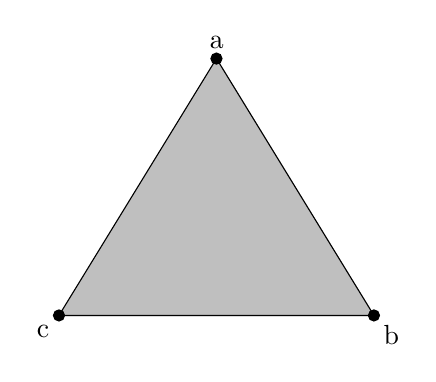
\begin{tikzpicture}
	\filldraw[lightgray] (-2,0)--(2,0)--(0,3.26210161512);
	\draw (-2,0)--(2,0)--(0,3.26210161512)--(-2,0);
	\filldraw (-2,0) node[below left] {c} circle (2pt);
	\filldraw (2,0) node[below right] {b} circle (2pt);
	\filldraw (0,3.26210161512) node[above] {a} circle (2pt);
\end{tikzpicture}
\end{center}
\[\mathcal{K}=\{a,b,c,ab,ac,bc,abc\}\]

There are no simplexes with order larger than $3$ hence like in previous examples $H_{n\geq 3}(\mathcal{K}) = 0$.
Hence we have:
\[0 \stackrel{\partial_3}{\longrightarrow} C_2 \stackrel{\partial_2}{\longrightarrow} C_1 \stackrel{\partial_1}{\longrightarrow} C_0 \stackrel{\partial_0}{\longrightarrow} 0\]
Where:
\[C_2 = \langle abc \rangle,\quad C_1 = \langle ab,ac,bc \rangle,\quad C_0 = \langle a,b,c \rangle\]
The $\ker$ and $\img$ are given bellow:
\begin{equation*}
\begin{aligned}
	&\img \partial_3 = 0 && \ker \partial_2 = 0\\
	&\img \partial_2 = \langle ab+bc+ca\rangle && \ker \partial_1 = \langle ab+bc+ca\rangle\\
	&\img \partial_1 = \langle a-b,a-c,b-c\rangle && \ker \partial_0 = \langle a,b,c\rangle\\
\end{aligned}
\end{equation*}

Gives the homologies:
\begin{equation*}
\begin{aligned}
	H_0(\mathcal{K}) =& \frac{\ker\partial_0}{\img\partial_1} = \frac{\langle a,b,c\rangle}{\langle a-b,a-c,b-c\rangle} = \langle a\rangle = \mathbb{Z}\\
	H_1(\mathcal{K}) =& \frac{\ker\partial_1}{\img\partial_2} = \frac{\langle ab+bc+ca\rangle}{\langle ab+bc+ca\rangle} = 0\\
	H_2(\mathcal{K}) =& \frac{\ker\partial_2}{\img\partial_3} = \frac{0}{0} = 0\\
\end{aligned}
\end{equation*}

\subsection{More Worked Examples}
\subsubsection{Tetrahedron without interior:}
\begin{center}
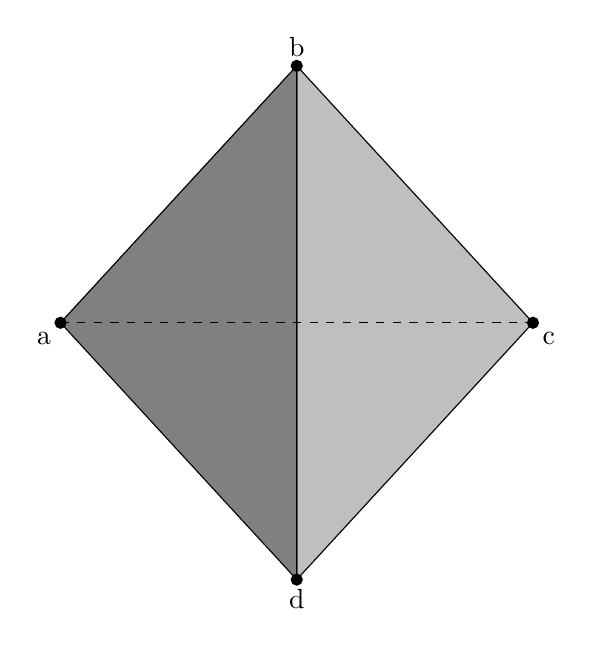
\begin{tikzpicture}
	\filldraw[gray] (-3,0)--(0,3.26210161512)--(0,-3.26210161512);
	\filldraw[lightgray] (0,3.26210161512)--(3,0)--(0,-3.26210161512);
	\draw (-3,0)--(0,3.26210161512)--(0,-3.26210161512)--(-3,0);
	\draw (3,0)--(0,3.26210161512)--(0,-3.26210161512)--(3,0);
	\draw[dashed] (-3,0)--(3,0);
	\filldraw (-3,0) node[below left] {a} circle (2pt);
	\filldraw (0,3.26210161512) node[above] {b} circle (2pt);
	\filldraw (0,-3.26210161512) node[below] {d} circle (2pt);
	\filldraw (3,0) node[below right] {c} circle (2pt);
\end{tikzpicture}
\end{center}
\[\mathcal{K}=\{a,b,c,d,ab,ac,ad,bc,cd,db,abc,abd,acd,cdb\}\]

We have:
\[0 \stackrel{\partial_3}{\longrightarrow} C_2 \stackrel{\partial_2}{\longrightarrow} C_1 \stackrel{\partial_1}{\longrightarrow} C_0 \stackrel{\partial_0}{\longrightarrow} 0\]
Where:
\[C_2 = \langle abc,abd,acd,cbd \rangle,\quad C_1 = \langle ab,ac,ad,bc,bd,dc, \rangle,\quad C_0 = \langle a,b,c \rangle\]
The $\ker$ and $\img$ are larger than previous examples,
despite being simplified,
and are given bellow:
\begin{equation*}
\begin{aligned}
	\img \partial_3 &= 0 \\
	\img \partial_2 &= \langle ab+bc+ca,ab+bd+da,ac+cd+da\rangle\\ 
	\img \partial_1 &= \langle a-b,a-c,a-d\rangle\\
	\ker \partial_2 &= \langle abc+adb+adc+dcb\rangle\\
	\ker \partial_1 &= \langle ab+bc+ca,ab+bd+da,ac+cd+da\rangle\\
	\ker \partial_0 &= \langle a,b,c,d\rangle\\
\end{aligned}
\end{equation*}

Gives the homologies:
\begin{equation*}
\begin{aligned}
	H_0(\mathcal{K}) =& \frac{\ker\partial_0}{\img\partial_1} = \frac{\langle a,b,c,d\rangle}{\langle a-b,a-c,a-d\rangle} = \mathbb{Z}\\
	H_1(\mathcal{K}) =& \frac{\ker\partial_1}{\img\partial_2} = \frac{\langle ab+bc+ca,ab+bd+da,ac+cd+da\rangle}{\langle ab+bc+ca,ab+bd+da,ac+cd+da\rangle} = 0\\
	H_2(\mathcal{K}) =& \frac{\ker\partial_2}{\img\partial_3} = \frac{\langle abc+adb+adc+dcb\rangle}{0} = \mathbb{Z}\\
\end{aligned}
\end{equation*}

\subsubsection{Mixed}
\begin{center}
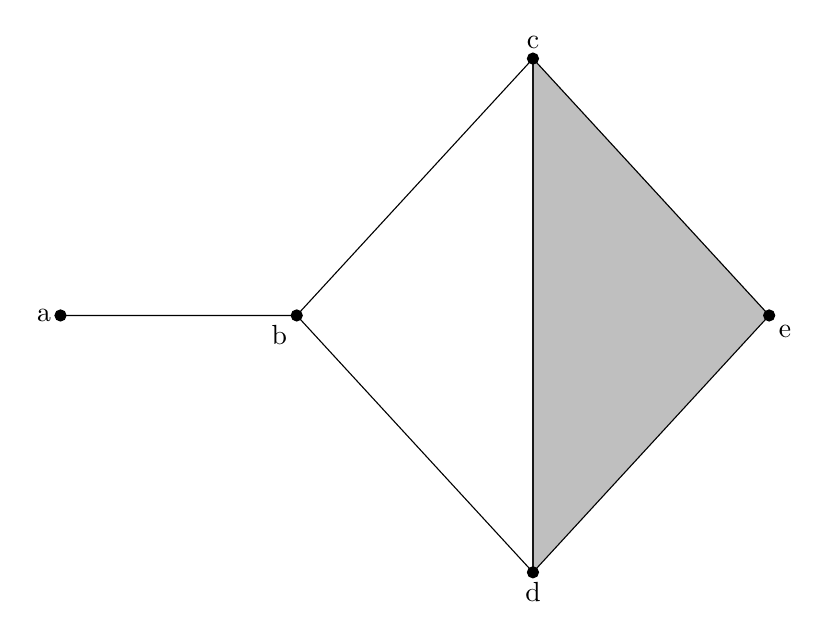
\begin{tikzpicture}
	\filldraw[lightgray] (3,0)--(0,3.26210161512)--(0,-3.26210161512);
	\draw (-6,0)--(-3,0)--(0,3.26210161512)--(0,-3.26210161512)--(-3,0);
	\draw (3,0)--(0,3.26210161512)--(0,-3.26210161512)--(3,0);
	\filldraw (-6,0) node[left] {a} circle (2pt);
	\filldraw (-3,0) node[below left] {b} circle (2pt);
	\filldraw (0,3.26210161512) node[above] {c} circle (2pt);
	\filldraw (0,-3.26210161512) node[below] {d} circle (2pt);
	\filldraw (3,0) node[below right] {e} circle (2pt);
\end{tikzpicture}
\end{center}
\[\mathcal{K}=\{a,b,c,d,e,ab,bc,bd,cd,ec,de,cde\}\]

We have:
\[0 \stackrel{\partial_3}{\longrightarrow} C_2 \stackrel{\partial_2}{\longrightarrow} C_1 \stackrel{\partial_1}{\longrightarrow} C_0 \stackrel{\partial_0}{\longrightarrow} 0\]
Where:
\[C_2 = \langle cde \rangle,\quad C_1 = \langle ab,bc,bd,cd,ec,de \rangle,\quad C_0 = \langle a,b,c,d,e \rangle\]
The $\ker$ and $\img$ are given bellow:
\begin{equation*}
\begin{aligned}
	&\img \partial_3 = 0 && \ker \partial_2 = 0\\
	&\img \partial_2 = \langle ce+ed+dc\rangle && \ker \partial_1 = \langle bc+cd+db, ce+ed+dc\rangle\\
	&\img \partial_1 = \langle a-b,b-c,b-d,c-d,e-c,d-e \rangle && \ker \partial_0 = \langle a,b,c,d,e\rangle\\
\end{aligned}
\end{equation*}

Gives the homologies:
\begin{equation*}
\begin{aligned}
	H_0(\mathcal{K}) =& \frac{\ker\partial_0}{\img\partial_1} = \frac{\langle a,b,c,d,e\rangle}{\langle a-b,b-c,b-d,c-d,e-c,d-e\rangle} = \langle a\rangle = \mathbb{Z}\\
	H_1(\mathcal{K}) =& \frac{\ker\partial_1}{\img\partial_2} = \frac{\langle bc+cd+db,ce+ed+dc\rangle}{\langle ce+ed+dc\rangle} = \langle bc+cd+db\rangle = \mathbb{Z}\\
	H_2(\mathcal{K}) =& \frac{\ker\partial_2}{\img\partial_3} = \frac{0}{0} = 0\\
\end{aligned}
\end{equation*}

\subsection{Interpretation of Simplicial Homology}
Let us summarise the worked example results:
\begin{center}
\begin{tabular}{|c|cccc|}
	\hline
	Complex & $H_0$ & $H_1$ & $H_2$ & $H_{n\geq 3}$ \\ 
	\hline
	Disconnected& $\mathbb{Z}^2$ &0&0&0 \\
	Triangle without interior& $\mathbb{Z}$ & $\mathbb{Z}$ & 0 & 0 \\
	Triangle with interior& $\mathbb{Z}$ & $0$ & 0 & 0 \\
	\hline
	\hline
	Tetrahedron without interior&$\mathbb{Z}$&0&$\mathbb{Z}$&0\\
	Mixed&$\mathbb{Z}$&$\mathbb{Z}$&0&0\\
	\hline
\end{tabular}
\end{center}
But what do they mean?
In a nutshell the power of $\mathbb{Z}$ corresponds to a specific topological feature called an $n$-hole.
A $0$-hole is a connected part,
a $1$-hole is a regular hole,
a $2$-hole is a cavity.
Hence the disconnected complex is made from two connected parts and the rest of one connected part.
And the triangle without an interior has a hole and the others don't.
\\

But why powers of  $\mathbb{Z}$?
And why does $\ker\partial_n / \img\partial_{n+1}$ give this result?
\\

The rigorous answer has to do with homotopy,
and the "Fundamental Homotopy Group" in particular,
which is the math of drawing loops on things then pulling them and then seeing where they get stuck.
Well worth a read but the basics are this:

For every hole you can wrap a loop around it multiple times and in both directions.
Wrapping it around clockwise once is identified with $1$,
wrapping it around counter-clockwise twice is identified with $-2$,
wrapping it around no hole is identified with $0$ since when the loop is pulled taut nothing gets stuck.

If there are two hole $a$ and $b$ then the loops are identified with an element over the free $\mathbb{Z}$-module over $\{a,b\}$.
For example $a+2b$ a clockwise loop over $a$ then two over $b$ and you can add two elements by making a cut in both loops then gluing them together (making sure you preserve orientation).

\begin{center}
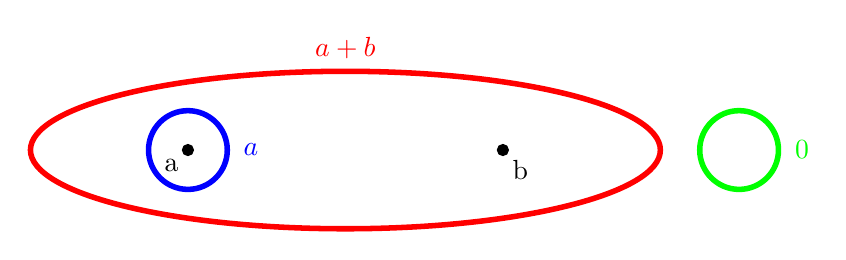
\begin{tikzpicture}
	\filldraw (-2,0) node[below left] {a} circle (2pt);
	\filldraw (2,0) node[below right] {b} circle (2pt);
	\draw[blue,line width=2pt] (-2,0) circle  [radius = 0.5cm];
	\draw[green,line width=2pt] (5,0) circle  [radius = 0.5cm];
	\draw[red,line width=2pt] (0,0) circle [x radius =4cm, y radius = 1cm];
	\node[blue] at (-1.2,0) {$a$};
	\node[green] at (5.8,0) {$0$};
	\node[red] at (0,1.3) {$a+b$};
\end{tikzpicture}
\end{center}

The free $\mathbb{Z}$-module over $\{a,b\}$ is isomorphic to $\mathbb{Z}^2$ because you need two integers to explain all the loops you can make over two holes that stay when taut,
which explains where the powers of $\mathbb{Z}$ came from.

$\ker\partial_n / \img\partial_{n+1}$ works because as noted in the definition of the chain group the elements of the chain group can jump around a bit.
But the requirement $\sigma\in\ker\partial_n$ makes it loop since it's boundary vanishes.
And $\img\partial_{n+1}$ are all the loops that have a higher order faces enabling a taut loop to move freely.
These steps combined give:
\begin{enumerate}
	\item $C_n$ contains all the loops but also completely broken path.
	\item Use $\ker\partial_n$ to get all elements of $C_n$ that are loops.
	\item Modulo $\img\partial_{n+1}$ to remove all loops that don't exit when pulled taut.
\end{enumerate}
\mbox 
Again, this explanation can be made more rigorous by studying homotopy.

\subsection{Boundaries and Cycles}
This is actually obvious,
but applying fundamental isomorphism theorem to $\partial_n:C_n\rightarrow C_{n-1}$ gives:
\[ B_{n-1} = \img\partial_n\cong \frac{C_n}{\ker\partial_n} = \frac{C_n}{Z_n} \]
This gives a new way to interpret $B_n$ based on $Z_n$,
and for $Z_n$ we only need to interpret $\sum_i (-1)^i\sigma_i =0$.
\\

It also makes me aware of how messy boundaries can be\footnote{And in math as well!}.
For example $\{ab,bc\}\subseteq C_1$ means $2a-b-c$ is and element of $B_0$ since you can take a chain of the edge from $b$ to $a$ and $c$ to $a$.

% Copyright 2023 Kieran W Harvie. All rights reserved.

\section{Matrix Function Evaluation using Cayley-Hamilton}
(This is something I'm 70\% sure I've seen before but I saw it again today).
(Assume the field is $\mathbb{R}$, don't feel like dealing with others).
\\

The Cayley-Hamilton theorem states that a matrix is the root of it's own characteristic equation.
A cool application of this is simplifying the evaluation of (analytic) matrix functions.
\\

Let $M$ be a matrix with characteristic polynomial $p$,
and eigenvalues $\lambda_i$ with multiplicity $m_i$.
Let the analytic function $f$ be given by:
\[f(x) = \sum_{k=0}^\infty f_kx^k\]
Define a new function $r$ that is interpolated on $\lambda_i$ such that:
\[0\leq k< m_i \Rightarrow\left.\frac{d^k f}{d x^k}\right|_{\lambda_i} =\left.\frac{d^k r}{d x^k}\right|_{\lambda_i}\]
This means that for some analytic function $q$ we have:
\[f(x) = q(x)p(x)+r(x)\]

Now convert these analytic functions to analytic matrix functions in the natural way.
From Cayley-Hamilton theorem we have:
\[f(M) = q(M)p(M)+r(M) = r(M)\]

\subsection{Worked Example}
Let $M$ be a $2\times 2$ matrix with two distinct eigenvalues.
Let $f(x) = \exp(tx)$ then:
\[r(x) = (x-\lambda_0)\frac{\exp(t\lambda_1)}{\lambda_1-\lambda_0}+(x-\lambda_1)\frac{\exp(t\lambda_0)}{\lambda_0-\lambda_1}\]
Hence:
\[f(M) = r(M) =(M-\lambda_0)\frac{\exp(t\lambda_1)}{\lambda_1-\lambda_0}+(M-\lambda_1)\frac{\exp(t\lambda_0)}{\lambda_0-\lambda_1} \]

\subsection{Original Application}
The original problem was to minimize:
\[f(X) = \sum_{k=0}^n\left|\left|\exp\left(\frac{2\pi}{k}B\right)A-X\right|\right|^2\]

Through some procedure similar to the above reasoning it was obtained:
\[\exp(\alpha B) = I+ \sin(\alpha)B+(1-\cos(\alpha))B^2\]

Hence:
\begin{equation*}
\begin{aligned}
&\sum_{k=0}^n\left|\left|\exp\left(\frac{2\pi}{k}B\right)A-X\right|\right|^2\\
=&\sum_{k=0}^n\left|\left|\left(I+\sin\left(\frac{2\pi}{k}\right)B+\left(1-\cos\left(\frac{2\pi}{k}\right)\right)B^2\right)A-X\right|\right|^2\\
=&\sum_{k=0}^n\left|\left|\bigg((I+B^2)A-X\bigg)+\left(\sin\left(\frac{2\pi}{k}\right)B+\cos\left(\frac{2\pi}{k}\right)B^2\right)A\right|\right|^2\\
\end{aligned}
\end{equation*}
The left term independent of $k$ and the right term is independent of $X$.
This means each term of the sum is minimized at:
\[X=(I+B^2)A\]
And since each term is minimized so is the whole sum.

% Copyright 2023 Kieran W Harvie. All rights reserved.

\section{Divisibility of $(p+1)(p-1)$}
It is well known that if $p$ is prime than either $p$ is a divisor of $6$ or has the remainder $1$ or $5$ when divided by $6$.
This can be verified by noting that a remainder of $0$,$2$, or $4$ would make $p$ divisible by $2$ and likewise for $0$ and $3$ for $3$.
\\

A cool corollary I saw today was that $p$ is a divisor of $6$ or $24$ is a divisor of $(p+1)(p-1)$.
This is also verified by cases:

\begin{center}
\begin{tabular}{|c|cccc|}
\hline
	$p\mod 12$&1&5&7&11\\
\hline
	$\gcd(p+1,12)$&2&6&4&12\\
	$\gcd(p-1,12)$&12&4&6&2\\
\hline
\end{tabular}
\end{center}

The converse isn't true.
Since $24\cdot 3 = 72$,
but $(7-1)(7+1) = 48 < 72$ and $(11-1)(11+1) = 120 > 72$.

% Copyright 2023 Kieran W Harvie. All rights reserved.

\section{Dominated Convergence Theorem}
Consider the following sequences of integrals:
\[I_n = \int_0^1\log(t)^2(1-t)^n\,dt\]
It's related to the Harmonic numbers,
which is why it peaked my interest,
but it was presented in context where we wished to understand its asymptotics.
\\

The book answer of expressing it in terms of hypergeometric functions will be skipped,
because it's boring.

\subsection{Cauchy-Schwartz}
\begin{equation*}
\begin{aligned}
\int_0^1\log(t)^2(1-t)^n\,dt \leq& \sqrt{\int_0^1\log^4(t)\,dt\int_0^1(1-t)^{2n}\,dt}\\
=&\sqrt{4! \frac{1}{2n+1}} \rightarrow 0
\end{aligned}
\end{equation*}
Which by the noticing the sign of $I_n$ and application of the sandwich theorem shows that $I_n \rightarrow 0$.

\subsection{Dominated Convergence Theorem}
As suggested by the section name, this is the result I really want to take notes about.
If a sequence of functions $f_n$ pointwise converge to $f$ and are dominated by some integrable function $g$ such that:
\[|f_n(t)| < g(t)\]
We have:
\[\int_S f_n\,d\mu \rightarrow \int_S f\,d\mu\]
Well rewrite the integral as:
\begin{equation*}
\begin{aligned}
\frac{n}{\log(n)^2}\int_0^1\log(t)^2(1-t)^n\,dt 
=& \int_0^1\left(\frac{(\log(nt)-\log(n)}{\log(n)}\right)^2\left(1-\frac{nt}{n}\right)^n\,d\,nt \\
=&\int_0^n\left(\frac{\log(t)}{\log(n)}-1\right)^2\left(1-\frac{t}{n}\right)^n\,dt \\
=& \int_0^\infty\chi_{[0,n]}(t)\left(1-\frac{\log(t)}{\log(n)}\right)^2\left(1-\frac{t}{n}\right)^n\,dt\\
\end{aligned}
\end{equation*}

Set:
\[f_n(t) = \overbrace{\chi_{[0,n]}(t)\left(1-\frac{\log(t)}{\log(n)}\right)^2}^{g_n(x)}\overbrace{\left(1-\frac{t}{n}\right)^n}^{h_n(t)}\]
We have (pointwise):
\[f_n(t) \rightarrow \exp(-t)\]
We also have $h_n(t) \leq \exp(-t)$ and $g_n(t) \leq (1-\log(t))^2$,
meaning:
\[|f_n(t)| \leq (1-\log(t))^2\exp(-t)\]
Giving the desired result
(Assuming we can show the RHS converges, 
which I'm pretty sure we can since near $0$ we have $\int (1-\log(t))^2\,dt = t(\log(t)^2-4\log(t)+5)$ and far away we have $\exp(-t)$).
\[\frac{n}{\log(n)^2}\int_0^\infty\log(t)^2(1-t)^n\,dt \rightarrow \int_0^\infty\exp(-t)\,dt = 1\]

% Copyright 2023 Kieran W Harvie. All rights reserved.

\section{Generated Subfield of Finite Fields}
Let the finite field $F$ have a set of elements $S$.
The set $\langle S \rangle$ whose elements are the sums of the products of powers of $S$:
\[\langle S \rangle = \left\{\sum_n\prod_i s_i^{p_{i,n}}\,|\,s_i\in S \text{ and } p_{i,n}\in \mathbb{Z}\right\}\cup\{0\}\]
For example if $S = \{s_0,s_1,s_2\}$ all of the following are elements of $\langle S \rangle$:
\[s_0+s_1+s_2,\quad s_0s_1s_2s_3,\quad 1+s_0+s_1s_2^7+s_0s_1s_2^2\]
(I use the $\langle \cdot \rangle$ notation because this is like generation,
one of the most irregular and abused words in algebra).
\\

The set inherits it's operations from $F$ and is clearly closed under addition and multiplication.
It also contains $1$ and its repeated sum, labeled $n$, by using $p_{i,n} = 0$:
\[n = \overbrace{(s_0s_1s_2)^0+(s_0s_1s_2)^0+\dots s(s_0s_1s_2)^0}^{n \text{ times}}\]

Given $q\in \langle S \rangle$ because there are a finite number of options for $nq$ the pigeonhole principle means there will eventually be $n > m+1$ such that:
\begin{equation*}
\begin{aligned}
nq =& mq\\
(n-m)q =& 0\\
q+(n-m-1)q=& 0\\
\end{aligned}
\end{equation*}
$(n-m-1)q$ which is the additive inverse of $q$.
Because $n-m-1 > 0$ it is an element of $\langle S \rangle$ and since $q$ is also an element by closure so is the inverse.
\\

Likewise for the multiplicative inverse:
\begin{equation*}
\begin{aligned}
q^n=&q^m\\
q\cdot q^{n-m-1}=&1
\end{aligned}
\end{equation*}
Hence $\langle S \rangle$ is a, not necessarily proper, subfield of $F$.

\subsection{$S=\{1\}$}
An important example is when $S=\{1\}$.
Let $n$ be the "lowest"\footnote{Yes I know I haven't defined that properly, but just figure it out.} where the pigeonhole principle whole applies:
\begin{equation*}
\begin{aligned}
	m + (n-m) =& n+(m-m)\\
	=& n \\
	=& m \\
\end{aligned}
\end{equation*}

The minimality\footnote{See previous footnote.} of $n$ makes $n-m$ non-zero making $n$ zero.
Hence $S\cong\mathbb{F}_{n}$.
\\

(This is sloppy even for quick notes)

\subsection{Dreams of a more rigor}
Let $R$ be a ring and let $\phi$ be a function from $\mathbb{Z}$ to $R$ such that:
\[\phi(1)=1_R,\quad \phi(n\pm 1) = \phi(n)\pm \phi(1_R)= \phi(n)\pm 1_R\]
$\phi$ is well-defined as you can find the value for any $n\in\mathbb{Z}$ by induction.
And the function only has one value at each $n$ since you can't change the value by "doubling back" on the induction:
\[\phi((n\pm 1)\mp 1) = \phi(n\pm 1)\mp 1_R = \phi(n)\pm 1_R\mp 1_R = \phi(n)\]

Induction on $n$ shows:
\begin{equation*}
\begin{aligned}
	\phi(n)+\phi(m) =& \phi(n\pm 1)\mp 1 +\phi(m) \\
	=& \phi(n\pm 1)+\phi(m\mp 1) \\
	=& \phi(n\pm 1 + m\mp 1) \\
	=& \phi(n+m) \\
\end{aligned}
\end{equation*}

Which can be used to further prove:
\begin{equation*}
\begin{aligned}
	\phi(n)\phi(m) =&(\phi(n\pm 1)\mp 1)\phi(m) \\
	=&\phi(n\pm 1)\phi(m)\mp\phi(m) \\
	=&\phi((n\pm 1)m)\mp\phi(m) \\
	=&\phi((n\pm 1)m\mp m) \\
	=&\phi(nm)\\
\end{aligned}
\end{equation*}

These identities,
combined $\phi$ being defined with $\phi(1)=1_R$,
shows that $\phi$ is a homomorphism.
\\

Which, 
by the first isomorphisms theorem for rings,
shows that the $\img\phi$ is a subring of $R$ and is isomorphic to $\mathbb{Z}/\ker \phi$.
This formalizes the concept of the $n$th sum of $1_R$,
and lets us manipulate it better.
\\

\textbf{Corollary:} If $R$ is finite then the additive group of $R$ is also finite.
Meaning $1_R$ has an order,
which we label $N$.
In this case $\ker\phi = N\mathbb{Z}$ giving:
\[\img\phi = \frac{\mathbb{Z}}{N\mathbb{Z}}\]
It's really easy to use Bézout's identity on these objects to show which ones are fields.

\subsection{Wedderburn's Little Theorem}
This is similar to Wedderburn's little theorem, 
that all finite domains are fields.
Wedderburn generalizes the subject to domains instead of field and thus has to use $q-q^n = 0$ and some polynomial analysis (Headache).
But reduces the results,
it doesn't discuss closure.
\\

Cool result,
I suggest looking it up.

% Copyright 2023 Kieran W Harvie. All rights reserved.

\section{Isomorphisms of the quotient rings of $\mathbb{Z}[X]$ }
While working elsewhere I thought that it's actually really easy to prove:
\[\gcd(a,d)=\gcd(b,d) \Rightarrow \exists z \in\mathbb{Z} \text{ such that } z\frac{a}{d}-\frac{b}{d} \in \mathbb{Z}\]
Using Bézout's identity.
\\

\subsection{The proof}
From Bézout's identity we know there exits $r,s$ in $\mathbb{Z}$ such that:
\[ra+sd = \gcd(a,d) = \gcd(b,d)\]
From the definition of $\gcd$ there exists $d'\in\mathbb{Z}$ such that:
\[b'\gcd(b,d) = b\]
Multiplying the first equation by $b'$ gives:
\[(rb')a+(sb')d = b'\gcd(b,d) = b\]
Hence:
\[(rb')\frac{a}{d}-b\frac{b}{d} = -(sb')\]
As required.
\\

Note that we can actually control the size, and hence sign, of $z$ by using the:
\[ra+sd = a(r+bk)+b(s-ak)\]
Trick, meaning we can force $z>0$ and hence $z\in\mathbb{N}$.

\subsection{The questions}
So this proof brings up some questions:
\begin{enumerate}
	\item Doesn't this prove that $\mathbb{Z}[X]/(dX-a) \cong \mathbb{Z}[X]/(dX-b)$?
	\item Couldn't this be generalized to Bézout Domains?
	\item What about the converse?
\end{enumerate}

\subsection{Question 1}
Let:
\[A = \mathbb{Z}[X]/(dX-a),\quad B =\mathbb{Z}[X]/(dX-b)\]
We can say $A$ and $B \subset \mathbb{Q}$ where we identity $X$ with $\frac{a}{d}$ and $\frac{b}{d}$ respectfully. 
But since we can find a linear relation between the two $X$s in terms, we need two relations but we can avoid division completely, of the sub-field $\mathbb{Z}$ I'd expect an isomorphism.
\\

Assume the $\gcd$ condition is meet and let $z_0$ and $z_1$ be the integers such that:
\[z_1\frac{a}{d}-\frac{b}{d} = -z_0\]
Equally written as:
\[d(z_1a+z_0)=b\]

\subsubsection{Attempt 1}
Define $\phi: B \rightarrow A$.
A ring homomorphism fixes $1$ and hence acts identically on the set generated by $1$,
that is $\mathbb{Z}$.
Since $a\in\mathbb{Z}$ hence:
\begin{equation*}
\begin{aligned}
	a =& \phi(a) \\
	=&\phi(dX) \\
	=&d\phi(X) \\
\end{aligned}
\end{equation*}
Suggesting a form for $\phi(X)$:
\[\phi(X) = z_1X+z_0\]
This is all the degrees of freedom we get since being a homomorphism requires:
\[\phi\left(\sum_np_nX^n\right) = \sum_n\phi(p_n)\phi(X)^n\]
Hence the suggested form is:
\[\phi\left(\sum_np_nX^n\right) = \sum_np_n(z_1X+z_0)^n\]

But dealing with showing homomorphism when dealing the canceling term isn't something I want to do.

\subsubsection{Attempt 2}
Define a function $\phi: \mathbb{Z}[X] \rightarrow B$ where:
\[\phi\left(\sum_np_nX^n\right) = \sum_np_n(z_1X+z_0)^n\mod (dX-b)\]
Then we can use the first isomorphism theorem of rings and only need to show that $\phi$ is surjective and has a kernel of  $\langle dX-a \rangle$.

% Copyright 2023 Kieran W Harvie. All rights reserved.

\section{Convex}
TODO: Flesh out, copy edit, and maybe include pictures for the geometric intuition in the cord section.
\\

In the section of Jensen's Inequality I defined a convex function $\phi$ on a set $X$ as one such that for $a_n\in X$ with $w_0+w_1 =1$ and $w_n \geq 0$ then we have:
\[\phi(w_0a_0+w_1a_1) \leq w_0\phi(a_0)+w_1\phi(a_1)\]
I've thought of another proof of the previous section but iterates over functions instead of points.
And we can use some geometry intuition (cords).
\\

\subsection{Cords}
First let me define a new function called the cord function that takes on an interval $[a,b] \subseteq X$:
\[C_{[a,b]}(x) = \phi(a)+(x-a)\frac{\phi(b)-\phi(a)}{b-a}\]
The convex property can be changed to:
\[x\in [a,b] \Rightarrow \phi(x) \leq C_{[a,b]}(x)\]

{\bf Lemma:}, if $x_0 \leq x_1 \leq x_2$ then:
\[ x\in [x_0,x_1] \Rightarrow C_{[x_0,x_1]}(x) \leq C_{[x_0,x_2]}(x)\]
and:
\[ x\in [x_1,x_2] \Rightarrow C_{[x_1,x_2]}(x) \leq C_{[x_0,x_2]}(x)\]
{\bf Proof:} Use $C_{[a,b]}(a) = \phi(a)$ or $C_{[a,b]}(b) = \phi(b)$ and $x_1 \in [x_0,x_2]$ with the definition of convexity.
\\

{\bf Lemma:}, if $a_0 \leq a_1 \leq b_1 \leq b_0$ then:
\[x\in [a_1,b_1] \Rightarrow C_{[a_1,b_1]}(x) \leq C_{[a_0,b_0]}(x)\]
{\bf Proof:} use the previous lemma with the triples form the quad inequality, then chain together the newer inequalities.
\\

Let:
\[\phi_{[A,B]}(x) = \begin{cases} C_{[A,B]}(x) & x\in [A,B] \\ \phi(x) &\text{else} \end{cases}\]
$\phi_{[A,B]}(x)$ is convex.
Prove this using the previous lemmas with the three cases (points same side, both sides, one in one out).

\subsection{The Cool Proof}
We want to show that for all $\sum_{i=1}^nw_i'=1$ and $w_i' \geq 0$:
\[\phi\left(\sum_{i=1}^nw_i'a_i\right) \leq \sum_{i=1}^nw_i'\phi(a_i)\]

Assume it works for $n-1$ points.
Take two points $(w_0,a_0)$ and $(w_1,a_1)$ and make a new convex function using the method from the previous section with $[x_0,x_1]$, then remove the two points and replace with $(w_0+w_1, \frac{w_0a_1+w_1a_1}{w_1+w_0})$.
Now we have a $n-1$ points,
and if you expand the algebra you get the correct form,
hence by induction you prove the initial result.

% Copyright 2023 Kieran W Harvie. All rights reserved.

\section{Jensen's Inequality}
A convex function $\phi$ on a set $X$ is one such that for $a_n\in X$ with $w_0+w_1 =1$ and $w_n \geq 0$ then we have:
\[\phi(w_0a_0+w_1a_1) \leq w_0\phi(a_0)+w_1\phi(a_1)\]
Jensen's Inequality states that expected value of the function is less then the function of the expected value:
\[\phi(\E(X)) \leq \E(\phi(X))\]

By multiplying the function by $-1$, we get the intuitive corollary that the inequality is reversed for concave functions.

\subsection{Generalization}
A more general form of convexity can be easily proved by induction.
\\

Assume that for some $n$ we have that for all $\sum_{i=1}^nw_i'=1$ and $w_i' \geq 0$:
\[\phi\left(\sum_{i=1}^nw_i'a_i\right) \leq \sum_{i=1}^nw_i'\phi(a_i)\]

Let $\sum_{i=1}^{n+1}w_i=1$ and $W = \sum_{i=1}^nw_i$ we have $w_{n+1}+W = 1$ and :
\begin{equation*}
\begin{aligned}
\phi\left(\sum_{i=1}^{n+1}w_ia_i\right) =&\phi\left(w_{n+1}a_{n+1}+W\sum_{i=1}^{n}\frac{w_i}{W}a_i\right) \\
\leq& w_{n+1}\phi(a_{n+1})+W\phi\left(\sum_{i=1}^{n}\frac{w_i}{W}a_i\right) \\
\leq& w_{n+1}\phi(a_{n+1})+W\sum_{i=1}^n\frac{w_i}{W}\phi(a_i) \\
\leq& \sum_{i=1}^{n+1}w_i\phi(a_i) \\
\end{aligned}
\end{equation*}

Viewing the weights as probabilities this form can directly be in interpreted as a discrete form of Jensen's Inequality.

\subsection{Mean Inequalities}
This can be directly applied to various mean inequalities.
\begin{equation*}
\begin{aligned}
	AM =& \frac{1}{n}\sum_{i=1}^{n}a_i \\
	RMS =& \sqrt{\frac{1}{n}\sum_{i=1}^na_i^2} \\
	GM =& \sqrt[n]{\prod_{i=1}^na_i}\\
\end{aligned}
\end{equation*}
Using $\phi(x)=x^2$,$w_i = \frac{1}{n}$ we directly get:
\[AM^2 \leq RMS^2\]
Using $\phi(x)=\log(x)$,$w_i = \frac{1}{n}$ we get:
\footnote{Remember that the inequality is reversed since $\log$ is concave}
\[\log(AM) \geq \log(GM)\]

Since both these functions are also monotonic the clean relations follow.

\subsection{Decision Theory} 
Interpret $\phi$ as a utility function then the convexity tells us whether we take the fixed $\E(X)$ or risk $X$.
Well if $\phi$ is convex then:
\[\phi(\E(X)) \leq \E(\phi(X))\]
And we should take the risk,
there is more expected utility taking the risk then the utility of $\E(X)$.

If $\phi$ is concave then we should not take the risk.

% Copyright 2023 Kieran W Harvie. All rights reserved.

\section{XOR hash}
Today I was presented with the following problem:
\\

Given an array with all integers $[1,100]$ with a single integer removed.
Assuming memory is limited, how do you efficiently determine the missing integer?
\\

The solution is to XOR all the elements of the array together.
Then XOR this with the known value for ALL the numbers between $[1,100]$.
The result will be the missing number.
\\

This problem seemed like a good introduction to hashes, like Zobrist, that XOR a bunch of info together.
The benefit of this approach is that the components can be added/removed by a XOR:
\[h(\{a_0,a_1\}) = h(\{a_0\})\XOR h(\{a_1\})\]

\subsection{Determining the constant}
It turns out its easy to calculate the constant for the original question by hand.
First define $T$ as:
\[T(n) = n \XOR T(n-1),\quad T(1) = 1\]
Then:
\[T(n) = \begin{cases}n&n \mod 4 = 0 \\1& n\mod 4 = 1\\ n+1 &n\mod 4 = 2\\ 0& n\mod 4 = 3\end{cases}\]
This can easily be proved by induction and remembering that for even $n$ we have:
\[n\XOR 1 = n+1\]

Because of the modularity you would expect there to be an expression for $T$ involving powers of the fourth root of unity ($i$): 
\[T(n) = \frac{1}{2} +\frac{1}{2}(1+(-1)^n)+\frac{1}{4}((i-1)(-i)^n-(i+1)i^n)\]
(Done on scrap paper, not double checked, close enough to see the form).
\\

While the hybrid function is probably a more useful form the last one involves complex numbers in a way I didn't expect.

\subsection{Homomorphic Hashing}
Those with mathematic training will notice that the property that make this approach work:
\[h(\{a_0,a_1\}) = h(\{a_0\})\XOR h(\{a_1\})\]
Has the same form as a homomorphism\footnote{"same form" as a "homomorphism", math pun intended} and would investigate homomorphic hash functions. 

Well the most influential definition of such a function happened in 2004 Krohn, Freedman and Mazieres proposed a definition of homomorphic hash function as function $H: V\rightarrow G$ such that:
\begin{itemize}
\item $H$ is collision resistant. Meaning we are unlikely to find $x$ and $y$ such that $H(x) = H(y)$.
\item $H$ is a homomorphism. Meaning $H(x+y) = H(x)+H(y)$ for all $x$ and $y$.
\end{itemize}

The main problem is defining $V$ that is compatible with the regiments on $H$.
Since we want to use the set union operator then the natural choice is $V = 2^S$ for some set $S$.
But our hash only has the same form as a homomorphism\footnote{haha} when the input sets are mutually exclusive.
In general we have:
\[H(S_0 \cup S_1) = H(S_0)\XOR H(S_1) \XOR H(S_0 \cap S_1)\]

We can make a collision resistant hash though.
Make $H$ uniformly distributed on $\mathbb{F}_2^{\log_2|S|}$ for $S$.
Then by induction and $x \XOR y = 0$ iff $x=y$ you can show that it stays uniform for $2^S$.
Meaning the chance of a collision is $\frac{1}{|S|}$

(This is actually a bound for when $|S|$ is a power of $2$, but you can figure out the rest)
\\

Homomorphic functions are still useful in cryptography though.

% Copyright 2023 Kieran W Harvie. All rights reserved.

\section{Quick Summary of Spaces}
A space is a collection of elements, often called points,
with some additional structure.
There are four main types of spaces that form a nice hierarchy,
that is that some types of spaces are always a subtype of other space.
\subsection{Hierarchy}
{\textbf{Topological Space: Neighbourhood}}
In a topological space the elements have a concept of "Neighbourhood",
that is the points which are adjacent to each point.
\begin{center}
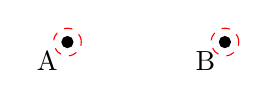
\begin{tikzpicture}
	\draw[dashed,red] (0,0) circle (5pt); 
	\filldraw (0,0) node[below left] {A} circle (2pt);
	\draw[dashed,red] (2,0) circle (5pt); 
	\filldraw (2,0) node[below left] {B} circle (2pt);
\end{tikzpicture}
\end{center}

{\textbf{Metric Space: Distance}}
In a metric space the element have a concept of distance to each other.
You can induce a neighbourhood by saying all points within a certain threshold distance to a point are in the neighbourhood of that point.
\begin{center}
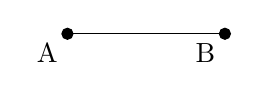
\begin{tikzpicture}
	\draw (0,0) -- (2,0);
	\filldraw (0,0) node[below left] {A} circle (2pt);
	\filldraw (2,0) node[below left] {B} circle (2pt);
\end{tikzpicture}
\end{center}

{\textbf{Normed Space: Length}}
In a normed space there is a concept of length of a point.
Shown here as their distance to some origin.
A distance can be induced by getting the length of an arrow going from A to B.
\begin{center}
\begin{tikzpicture}
	\draw[->] (0,0) -- (0,3.8);
	\draw[->] (0,0) -- (1.9,2.9);
	\filldraw (0,0) node[below] {O} circle (2pt);
	\filldraw (0,4) node[left] {A} circle (2pt);
	\filldraw (2,3) node[right] {B} circle (2pt);
\end{tikzpicture}
\end{center}


{\textbf{Inner-product Space: Projection}}
An inner product space has a concept of projecting one element on another.
You can induce a length by projecting an object onto itself.
\begin{center}
\begin{tikzpicture}
	\draw[->] (0,0) --(0,4.8);
	\draw[->] (0,0) -- (1.9,1.9);
	\draw[red,dashed] (2,2) -- (0,4);
	\draw (1.7,2.3) -- (1.4,2) -- (1.7,1.7);
	\filldraw (0,0) node[below] {O} circle (2pt);
	\filldraw (0,5) node[left] {A} circle (2pt);
	\filldraw (2,2) node[right] {B} circle (2pt);
	\filldraw (0,4) node[left] {B$'$} circle (2pt);
\end{tikzpicture}
\end{center}

\subsection{Euclidean}
Euclidean space is a normed space on $\mathbb{R}^n$ where the inner product is given by $\sum_k A_kB_k$.
This naturally induces a metric on $\mathbb{R}^n$.

The reason we care about the metric of Euclidean space is because all normed spaces have a form of the Pythagorean theorem.
Making metric space the most endowed space we can easily start thinking about non-Euclidean space.

This sucks because most talk about non-Euclidean space talks about "parallel lines" which makes one naturally think about angles and hence an inner product.
But no, instead we have the concept of a geodesic.
A geodesic is a curve that is locally distance minimizing.
This locality comes from the topology, and means that for all points $\gamma(t_1)$ and $\gamma(t_0)$ on the curve $\gamma$ such that they are in the same neighbourhood satisfy:
\[ d(\gamma(t_1),\gamma(t_0)) = k|t_1-t_2|\]

\subsection{non-Euclidean}
Quick rundown of some attempts of non-Euclidean geometries:

Pseudo-Euclidean: Like how we defined Euclidean Space was defined with an inner product we define a new structure with a different quadratic form.
\\

Riemann Manifold: A Manifold is a space that is "locally Euclidean". And a Riemann Manifold is one where this inner-product in the local Euclidean space is always positive.\\

Pseudo-Riemann Manifold: Like A Riemann Manifold but the inner-product is only required to be non-degenerate. I think this includes Pseudo-Euclidean space, but haven't put much thought into it.

% Copyright 2023 Kieran W Harvie. All rights reserved.

\section{p-adic numbers}
\subsection{Valuation}
A function $v$ of a field is called a valuation if:
\begin{equation*}
\begin{aligned}
	v(x) =& \infty \text{\quad iff } x = 0 \\
	v(xy) =& v(x)+v(y) \\
	v(x+y) \geq& \min(v(x),v(y)) \text{\quad with equality if } v(x) \neq v(y) \\
\end{aligned}
\end{equation*}
(Note that the codomain is only required to be an abelian totally ordered group extended with $\infty$,
But I will treat is as the natural numbers.)
\\

There are three immediate corollaries of the definitions.

{\textbf{1:}}By induction on the inequality we have:
\[v\left(\sum_k x_k\right) \geq \min\left(\bigcup_k \{v(x_k)\}\right)\]

{\textbf{2:}} By setting $x=y=1$ in the second equality we have $v(1)=2v(1)$ and hence $v(1) = 0$.

{\textbf{3:}} By setting $xy=1$ in the second equality we have $v(1/x)=-v(x)$.

\subsection{p-adic numbers}
Interestingly, the amount of times a prime $p$ divides a rational number $x$ is a valuation.
Let $x = p^n\frac{a}{b}$ where $a$ and $b$ are coprime, then $v_p(x) = n$ is a valuation.
(Assuming you set $v_p(0) = \infty$).
This is easy to prove, if you need help remember that for a prime $p$ we have: $p | ab \Rightarrow p|a$ or $p|b$.
\\

The reason this is interesting is because $|x|_p = p^{-v_p(x)}$ is a metric on $\mathbb{Q}$.
Meaning we can make a new field $\mathbb{Q}_p$ by taking all the limits in $\mathbb{Q}$ as we would nomarlly do to make $\mathbb{R}$ with $|\cdot|$.
And through something called Ostrowski's theorem becomes a lot more motivated and less arbitrary way to complete $\mathbb{Q}$.
\\

But the valuation alone also provides two cool proofs that simplify previous proofs.


\subsection{Irrationality of $\sqrt{2}$}
Consider the equation:
\[x^2 = 2\]
Valuating both sides gives:
\[2v_2(x) = 1\]
But $v_2(x)$ is an integer for all rational $x$ hence the LHS is always even but the right is odd.
Hence there is no $x$ satisfying the equation and $\sqrt{2}$ is irrational.

\subsection{Valuation of the Harmonic Numbers}
The valuation of harmonic numbers is given by $v_2(H_n) = -\lfloor \log_2(n) \rfloor$.
\\

{\textbf{Lemma:}}
Let $k$ be the power of the largest power of $2$ less than $n$, i.e. $k = \lfloor \log_2(n) \rfloor$.
Let $S$ be the set $[1,n]$ excluding $2^{k}$, then from the maximality of $k$ we have:
\[\max(v_2(S)) \leq k-1\]
Since if we assume there is an $s\in S$ such that $v_2(s) > k-1$ with the codomain of $v_2$ being integers means $v_2(s) \geq k$.
This means there exists an integers $a$ and $b$ coprime to each other and $2$ such that $s= 2^k\frac{a}{b}$.
$s$ being a positive integer means $b=1$. 
$a\neq1$ since it would make $s=2^k$, which was excluded from $S$.
But $a\geq2$ would means $2^{k+1} \in S$, contradicting the maximality of $k$.
\\

Now $H_n$ can be written as the following sum:
\[H_n = \sum_{s\in S} \frac{1}{s} + 2^{-k}\]

Where the valuation of  first term is bound by:
\begin{equation*}
\begin{aligned}
	v_2\left(\sum_{s\in S}\frac{1}{s}\right) \geq& \min\left\{v_2(1/s)\,|\,s\in S\right\} \\
	=& \min\left\{-v_2(s)\,|\,s\in S\right\} \\
	=& -\max\left\{v_2(s)\,|\,s\in S\right\} \\
	=& -k+1 \\
\end{aligned}
\end{equation*}

Hence the valuations are not equal since:
\[v_2(2^{-k}) = -k < -k+1 \leq v_2\left(\sum_{s\in S}\frac{1}{s}\right)\]

Hence

\begin{equation*}
\begin{aligned}
	v_2(H_n) =& \min\left\{ v_2\left(\sum_{s\in S}\frac{1}{s}\right) , v_2(2^{-k})\right\} = -k\\
\end{aligned}
\end{equation*}

As required.
\\

Note that for $n \geq 2$ we have $k \geq 1$ and hence $v_2(H_n) \leq -1$ meaning $H_n$ isn't an integer for $n\neq1$

\subsection{Valuation of the Harmonic Numbers v2}
I think the lemma's of the previous proof can be separated and cleaned up.

{\textbf{Lemma:}} Let $S$ be a subset of the $v$'s domain with an element $s_0\in S$ such that:
\[v(S\textbackslash\{s_0\}) > v(s_0)\]
Then:
\[v\left(\sum_{s\in S}s\right) = v(s_0)\]
{\textbf{Proof:}} Plugging the inequality into the valuation inequality axiom gives:
\[ v\left(\sum_{s\in S\textbackslash\{s_0\}}s\right) \geq v(S\textbackslash\{s_0\}) > v(s_0)\]
Hence the term of the far left and far right are not equal meaning:
\begin{equation*}
\begin{aligned}
	v\left(\sum_{s\in S}s\right) =& v\left(s_0+\sum_{s\in S\textbackslash\{s_0\}}s\right) \\
	=& \min\left\{v(s_0),v\left(\sum_{s\in S\textbackslash\{s_0\}}s\right)\right\} \\
	=&v(s_0)\quad \square\\
\end{aligned}
\end{equation*}

{\textbf{Lemma:}} If $n \in \mathbb{N}$ then $v_p(n) \leq \log_p(n)$ with equality iff $n$ is a power of $p$.

{\textbf{Proof:}} Equality in the case of $n$ being a power is trivial.
Now consider $n$ not a power of $2$ meaning $n = a\,p^{v_p(n)}$ where $a > 1$, hence:
\[p^{v_p(n)} <  n = p^{\log_p(n)} \]
$\log_p$ is strictly monotonic, hence:
\[{v_p(n)} < {\log_p(n)} \]

{\textbf{Lemma:}} If $n \in \mathbb{N}$ then $v_2(n) \leq \lfloor \log_2 (n) \rfloor$ with equality iff $n$ is a power of $2$.

{\textbf{Proof:}} Equality in the case of $n$ being a power is trivial.
Assume $n$ isn't a power of $2$ then:
\[n \geq 3\cdot 2^{v_2(n)}\]
Hence:
\begin{equation*}
\begin{aligned}
	\log_2(n) \geq& \log_2(3)+v_2(n) \\
	\log_2(n)-\log_2(3) \geq& v_2(n) \\
	\lfloor\log_2(n)-\log_2(3)\rfloor \geq& \lfloor v_2(n) \rfloor \\
\end{aligned}
\end{equation*}

Since $\log_2(3) > 1$ we have:
\[\lfloor \log_2 (n) \rfloor > \lfloor\log_2(n)-\log_2(3)\rfloor\]
And $v_2(n)$ is an integer, hence:
$\lfloor \log_2 (n) \rfloor > v_2(n)\quad \square$
\\

Note that this can't be generalized to larger $p$ since the logarithm being less than one isn't guaranteed.
Compare with $p=3$ with $v_3(6) = 1 = \lfloor \log_3(6) \rfloor$ because $\log_3(2) < 1$.
Note to the previous note, in this case you can say $v_3(n) \leq \lfloor \log_p(n) \rfloor$ iff $n$ is a power of $3$ or even, which is still \emph{kind of} cool.

{\textbf{Lemma:}} Let $S_n = \left\{k^{-1} | 1 \leq k \leq n\right\}$ and $k_0 = \lfloor\log_2 n\rfloor$.
Then $2^{-k_0} \in S$ and satisfies:
\[v_2(S_n\textbackslash\{2^{-k_0}\}) > v_2(2^{-k_0})\]

{\textbf{Proof:}} $2^{k_0} = 2^{\lfloor \log_2 n \rfloor} \leq 2^{\log_2 n} = n$ hence $2^{-k_0} \in S$.
Now consider $s\in S$ then $s^{-1} \in \mathbb{N}$ which from the previous lemma means:
\[ v_2(s^{-1}) \leq \lfloor \log_2(s^{-1})\rfloor \leq \lfloor \log_2(n)\rfloor = k_0\]
With equality iff $s^{-1}$ is a power of $2$.
It's can't be a larger power than $2^{k_0}$ since $2^{\lfloor \log_2 (n) \rfloor}$ is the largest power less than or equal to $n$.
But from the definition of $S_n\textbackslash\{2^{-k_0}\}$ it can't be the same power.
Hence $s^{-1}$ can only be a lower power making the final inequality strict anyway.
Hence:
\[ v_2(s^{-1}) < k_0 \Rightarrow v_2(s) > -k_0 = v_2(2^{-k_0})\quad \square\]

Noting that $H_n = \sum_{s\in S_n}s$ means the proof that $v_2(H_n) = -\lfloor \log_2 (n) \rfloor$ follows immediately from the first and last lemmas.

%% Induction is a bad way to prove this so it has been commented out %%
%This can be proved by induction on $k$.
%\\
%
%{\textbf{Base Case:}} The base case is quite direct:
%\begin{equation*}
%\begin{aligned}
%	k=0 \Rightarrow\, & n \in [1,2) \\
%	\Rightarrow\, & n = 1 \\
%	\Rightarrow\, & H_1 = 1 \\
%	\Rightarrow\, & v_2(H_1) = 0 \\
%\end{aligned}
%\end{equation*}
%
%{\textbf{Induction:}}
%Assume that $v_2(H_n) = -k'$ when $n\in[2^{k'}, 2^{k'+1})$ for $k' < k$:
%Hence $2^{k}-1$ is in the previous step, giving $v_2(H_{2^{k}-1}) = -k+1$.
%Which is clearly not equal to $v_2(2^k)$ meaning applying the second valuation property gives:
%
%\begin{equation*}
%\begin{aligned}
%	v_2(H_{2^k}) =& v_2(H_{2^k-1} + 2^{-k}) \\
%	=& \min\big(v_2(H_{2^k-1}),v_2(2^{-k}\big)) \\
%	=& \min(-k+1,-k)\\
%	=& -k\\
%\end{aligned}
%\end{equation*}
%
%Now assume $n \in (2^k,2^{k+1})$ then $v_2(\frac{1}{n}) > -k$ since $n$ is divisible by $p$ less then $k$ times.
%
%\begin{equation*}
%\begin{aligned}
%	v_2(H_n) =& v_2(H_{2^k} + \sum_{l=2^k+1}^{n}\frac{1}{l}) \\
%\end{aligned}
%\end{equation*}

% Copyright 2023 Kieran W Harvie. All rights reserved.

\section{Padé Approximant}
We wish to approximate a function $f$ by creating a rational function that agrees with $f$'s first $N$ derivatives at zero.

Let $T_N$ be the $N$th degree Maclaurin series of $f$.
Consider the steps of finding the polynomial greatest common division by the extended Euclid algorithm of $T_N$ with $x^{N+1}$ where we prematurely stop:
\begin{equation*}
\begin{aligned}
	x^{N+1} =& 1\cdot x^{N+1} +& 0\cdot T_N(x) \\
	T_N(x) =& 0\cdot x^{N+1} +& 1\cdot T_N(x) \\
	r_1(x) =& 1\cdot x^{N+1} + & -q_1(x)\cdot T_N(x) \\
	& \vdots &\\
	P(x) =& K(x)x^{N+1} + & Q(x) T_N(x) \\
\end{aligned}
\end{equation*}

By inspection we get the useful relation:
\[P(x)/Q(x) \equiv T_N(x) \mod x^{N+1}\]

Hence satisfying the original objective.
Note that we can chose decrease the degree of $P$ by simply continuing the algorithm.

\subsection{The Reverse}
Say I want to do the reverse, that I have $f = g/h$ where I have the power series for $g$ and $h$ but want to effectively find $f$
We have:

\begin{equation*}
\begin{aligned}
	x^{N+1} =& 0\cdot f(x) + &1\cdot x^{N+1}\\
	g(x) =& h(x)\cdot f(x) +& 0\cdot x^{N+1} \\
\end{aligned}
\end{equation*}

You can remove some higher term of $f$ into a residue function $K$ on $x^{N+1}$, since we don't really care about it.

\subsection{Differential}
What if $g$ and $h$ are related buy a differential equation?
We can use it like how we used the quotient-remainder equation.
The derivative is linear after all.



\subsection{Chinese Remainder Theorem}
Since I have modulo relations can I combine them with the Chinese Remainder Theorem?
The moduli will have to be pairwise coprime $(x-a_i)^n$ stand out.

% Copyright 2023 Kieran W Harvie. All rights reserved.

\section{Isosets}
Consider the function $f: \mathbb{R}^n \rightarrow \mathbb{R}$ let the isosets\footnote{Not the proper name, but I can't recall the proper name right now.} be sets $S$ in the domain of $f$ such that $f(S)$ is constant.
\\

Given some isoset $S$ and point $x \in \mathbb{R}^n$ of $f$ we want some kind of function that returns some type of measure $d \in \mathbb{R}$ of the distance of $x$ to $S$.
This function will be used in fragment shader rendering, which is why the mission statement is so vague.
We only need some general measure since it's better to efficiently get that measure and tweak coefficients then to get something perfectly accurate.
\\

A particular application is the $n=2$ case where we are looking to find the distance for the contour line.

\subsection{Naïve Solution}
The first idea is to compare the distance of $f(x)$ to $f(S)$ to $d$:
\[ d = |f(x)-f(S)|  \]
The problem with this solution is that the measure changes as a function of $|\nabla f(x)|$.
That is to say that the faster $f$ changes at $x$ the closer $x$ has to be to $S$ to get the same value of $d$.
\\

This method might work for some shader effects but not others.
For example it won't work to draw a constant width contour as the width would be inversely proportional to $|\nabla f(x) |$

\subsection{Better Solution}
If the underestimation is proportional to $|\nabla f(x)|$ the obvious solution is to divide by $|\nabla f(x)|$:
\[ d = \frac{|f(x)-f(S)|}{|\nabla f(x)|}\]
This is the solution currently used but deserves more analysis.
\\

For starters consider the case that $x$ is near the point $s \in S$.
Then $\nabla f(s)$ points away from $S$, that is that if a tangent to $S$ exists at $s$ then $\nabla f(s)$ is at orthogonal to the tangent, by definition of $S$ being a set such that $f$ is constant.
The combination of orthogonality and closeness lets us recover the original expression by use of the tangent surface:
\begin{equation*}
\begin{aligned}
	f(x) =& f(s)+(x-s)\cdot \nabla f(s) \\
	|f(x)-f(s)| =& |(x-s) \cdot \nabla f(s) |\\
	=& |x-s||\nabla f(s)| \\
	\frac{|f(x)-f(s)|}{|\nabla f(s) |} =& |x-s| \\
\end{aligned}
\end{equation*}
\\

Now consider the case where $x$ is not close to $S$ and the use case of drawing a constant width contour line.
Under what conditions do we avoid a false positive?
(That is the function thinks $x$ is closer than it is.)
Well we need some constraints on the rate at which $\nabla f(x)$ can grow.
To see this consider a point far away from $S$ but whose rate of change is very slow between most of $x$ and $s$, so that $|f(x) - f(s)|$ is small, but suddenly increases at $x$, such that $|\nabla f(x)|$ is large.
This causes their ratio to be small despite $|x-s|$ being large, false saying $x$ should be colored as part of the contour line.
If we reverse the set up, rate of change is large at first then slow, we will get a false negative.
(That the point is further than we think it is) 
\\

To see how a constraint would be useful, consider the following one: 
\[ |\nabla f(x+d)| \leq k|d||\nabla f(x)|\]
\begin{equation*}
\begin{aligned}
	|f(x)-f(s)| =& \left|\int_{0}^{1}\nabla f(x + (s-x)t) \cdot (s-x) \,dt\right| \\
	=& \left|(s-x)\cdot\int_{0}^{1}\nabla f(x + (s-x)t) \,dt\right| \\
	\leq& |(s-x)|\left|\int_{0}^{1}\nabla f(x + (s-x)t) \,dt\right| \\
	&\text{Cauchy-Schwartz} \\
	\leq& |(s-x)|\int_{0}^{1}\left|\nabla f(x + (s-x)t) \right|\,dt \\
	&\text{ML Bound} \\
	\leq& |(s-x)|\int_{0}^{1}k|(s-x)t||\nabla f(x)|\,dt \\
	\frac{|f(x)-f(s)|}{|\nabla f(x)|} \leq& \frac{k}{2}|s-x|^2 \\
\end{aligned}
\end{equation*}

This avoids a false negative as $x$ must be at least $ \sqrt{\frac{2d}{k}}$ away.

To-do: we need a inequities like $d \geq p(|x-s|)$ to get a bound on false positives.
\\
The condition:
\[ |\nabla f(x+d)| \leq k|d|+|\nabla f(x)|\]
Gives:
\[d \leq |x-s|\left(1+\frac{|x-s|}{|\nabla f(x)|}\right)\]

% Copyright 2023 Kieran W Harvie. All rights reserved.

\section{Lagrange Multiplier}
Recall that local extrema $x$ of the function $f :\mathbb{R}^n \rightarrow \mathbb{R}$ subject to contrasts $g_i$ satisfy:
\[\nabla f(x) = \sum_i \lambda_i \nabla g_i(x)\]

The core observation is that if $\nabla f$ has a component outside the span of ${\nabla g_i}$ then you can move in that direction while keeping $g_i$'s constant, contradicting the point being an extrema.
\\

But the actual constants $\lambda_i$ have a useful interpretation as the rate the value of $f$ at the extrema changes as the constant $g_i$ changes.
To see this pick a particular $g_j$ and construct a $d$ such that:
\[d\cdot \nabla g_i = D\delta_{i,j}\]
You can achieve this by iteratively removing components in some matter like the following:
\[d_0 = \nabla g_0,\, d_{n+1} = d_n -d_n\cdot\nabla g_n\]

Now scale $d$ down such that functions around the extrema can be approximated through targets\footnote{Those so inclined are free to chase $\epsilon - \delta$'s}.
We have:
\begin{equation*}
	\begin{aligned}
		g_i(x+d) =& g_i(x)+d\cdot\nabla g_i(x)\\
		=& g_i(x) + D\delta_{i,j} \\
		f(x+d) =& f(x)+d\cdot\nabla f(x) \\
		=& f(x) + \sum_i \lambda_i d \cdot \nabla g_i(x) \\ 
		=& f(x) + D\lambda_j \\
		\nabla f(x+d) =& \nabla(f(x)+D\lambda) \\
		=& \nabla f(x) \\
		=& \sum_i \lambda_i \nabla g_i(x) \\
		=& \sum_i \lambda_i \nabla \big(g_i(x+d) - D\delta_{i,j}\big) \\
		=& \sum_i \lambda_i \nabla g_i(x+d)\\
	\end{aligned}
\end{equation*}
From the these equation we can see that $x+d$ satisfy the requirement to be an extrema.
We can also see that a change of $D$ in $g_i$ created a change of $\lambda_j D$ in the value at the extrema, hence giving a rate of change of $\lambda_j$.
\\

To-Do: Add and example of minimizing height when the two contrasts are parabolic and linear.
(You will need to use logs to get the change for the parabola to be a change in it's width and not height.)

% Copyright 2023 Kieran W Harvie. All rights reserved.

\section{Interest Identities}
Let $P$ be the principle invested at a rate of $r$.
Consider four different investment scenarios:
\begin{itemize}
	\item Not invested: $P_0 = P$.
	\item Fully Invested at the beginning, one instalment at the end:
		\[P_1 = (1+r)P\]
	\item Continuously invested, continuous installments:
		\[P_2 = \lim_{n\rightarrow\infty}\sum_{k=0}^n\frac{P}{n}\left(1+\frac{r}{n}\right)^k = \frac{\exp(r)-1}{r}P\]
	\item Fully Invested at the beginning, continuous instalments: 
		\[P_3 = \lim_{n\rightarrow \infty}P\left(1+\frac{r}{n}\right)^n = \exp(x)P\]
\end{itemize}

Interestingly the relative size of $P_2$ and $P_1$ depend on $r$.
$P_1$ starts on $P_2$ but switches as $r$ increases.\\

$P_3$ is always the best, the proof for $P_1$ and $P_0$ are obvious.
$P_3 > P_2$ follows from:
\[0 < \int_0^rt\exp(t)\,dt = \big[(t-1)\exp(t)\big]_0^r = (r-1)\exp(r)+1\] \\

The following interesting identities hold:
\[P_3 = rP_2+P_0\]
\[P_3-P = r(P_2-P) + (P_1-P)\]
The breaks first neatly breaks $P_3$ into a nice linear sum.
The second does similar for the profit of the investment, total yield minus principle.


\chapter{Pre 2023}
% Copyright 2023 Kieran W Harvie. All rights reserved.

\section{Hermite Generating Functions}
\subsection{General}
\begin{equation*}
\begin{aligned}
	\sum_{n=0}^{\infty}\frac{H_n(x)}{n!}t^n =& \exp(2xt-t^2) \\
	=&\left(\sum_{n=0}^{\infty}\frac{(2x)^n}{n!}t^n\right)\left(\sum_{n=0}^{\infty}\frac{(-1)^n}{n!}(t^2)^n\right)\\
	=&\left(\sum_{n=0}^{\infty}\frac{(2x)^{2n}}{(2n)!}t^{2n}+2xt\sum_{n=0}^{\infty}\frac{(2x)^{2n}}{(2n+1)!}t^{2n}\right)\left(\sum_{n=0}^{\infty}\frac{(-1)^n}{n!}(t^2)^n\right)\\
	\frac{H_{2n}(x)}{(2n)!} =& \sum_{k=0}^{n}\frac{(4x^2)^k}{(2k)!}\frac{(-1)^{n-k}}{(n-k)!} \\
	H_{2n}(x)=& (-1)^n\sum_{k=0}^{n}(-4x^2)^k\frac{(2n)!}{(2k)!(n-k)!} \\
	=& (-1)^n\sum_{k=0}^{n}(-4x^2)^k\frac{(2n)!}{(2k)!(2(n-k))!}\cdot2^{n-k}\prod_{l=1}^{n-k}(2l-1)\\
	=& \sum_{k=0}^{n}x^{2k}2^{n+k}\binom{2n}{2k}\prod_{l=1}^{n-k}(1-2l)\\
	=& \sum_{k=0}^{n}x^{2k}2^{n+k}\binom{n}{k}\prod_{l=k+1}^{n}(1-2l)\\
%	=& (-1)^n(2n)!\sum_{k=0}^{n}\frac{(-4x^2)^k}{(2k)!(n-k)!} \\
%	=& \frac{(-1)^n(2n)!}{n!}\sum_{k=0}^{n}(-x^2)^k\binom{n}{k}\frac{4^kk!}{(2k)!}\\
%	=& (-1)^n\sum_{k=0}^{n}(-x^2)^k\binom{n}{k}\binom{2n}{n}\binom{2k}{k}^{-1}\frac{4^krn!}{k!}\\
\end{aligned}
\end{equation*}

\subsection{Multidimensional}
Let $T_0 = \sum_{i\in\mathbb{Z}\backslash n\mathbb{Z}}t_i $ and  $T_1 = T_0^2-\sum_{i\in\mathbb{Z}\backslash n\mathbb{Z}}t_i^2 = \sum_{(i,j)\in(\mathbb{Z}\backslash n\mathbb{Z})^2,i\neq j}t_it_j $

\begin{equation*}
\begin{aligned}
	&\sum_{\sigma \in \mathbb{N}^n}\left(\prod_{i\in\mathbb{Z}\backslash n\mathbb{Z}}\frac{t_i^{\sigma_i}}{\sigma_i!}\right)\int_{-\infty}^{\infty}\exp(-x^2)\left(\prod_{i\in\mathbb{Z}\backslash n\mathbb{Z}}H_{\sigma_i}(x)\right)\,dx\\
	=&\int_{-\infty}^{\infty}\exp(-x^2)\sum_{\sigma \in \mathbb{N}^n}\left(\prod_{i\in\mathbb{Z}\backslash n\mathbb{Z}}H_{\sigma_i}(x)\frac{t_i^{\sigma_i}}{\sigma_i!}\right)\,dx\\
	=&\int_{-\infty}^{\infty}\exp(-x^2)\prod_{i\in\mathbb{Z}\backslash n\mathbb{Z}}\left(\sum_{\sigma \in \mathbb{N}^n}H_{\sigma_i}(x)\frac{t_i^{\sigma_i}}{\sigma_i!}\right)\,dx\\
	=&\int_{-\infty}^{\infty}\exp(-x^2)\prod_{i\in\mathbb{Z}\backslash n\mathbb{Z}}\exp(2xt_i-t_i^2)\,dx\\
	=&\int_{-\infty}^{\infty}\exp(-x^2)\exp\left(2x\sum_{i\in\mathbb{Z}\backslash n\mathbb{Z}}t_i-\sum_{i\in\mathbb{Z}\backslash n\mathbb{Z}}t_i^2\right)\,dx\\
	=&\int_{-\infty}^{\infty}\exp\left(-x^2+2xT_0-T_0^2+T_1\right)\,dx\\
	=&\exp(T_1)\int_{-\infty}^{\infty}\exp(-(x-T_0)^2)\,dx\\
	=&\exp(T_1)\sqrt{\pi}\\
\end{aligned}
\end{equation*}

For $n\geq 4$ we have 
\[t_0t_1t_2t_3=(t_0t_1)(t_2t_3)=(t_0t_2)(t_1t_3)\]
But for $n = 3$ we have a unique way to get each term in the generating function from the final product as any two pairs share an element.
On the condition that $s \geq t_n$ and is an integer, this uniqueness is given by:

\begin{equation*}
\begin{aligned}
	t_0^{p_0}t_1^{p_1}t_2^{p_2} =& (t_0t_1)^{\frac{p_0+p_1-p_2}{2}}(t_0t_2)^{\frac{p_0+p_2-p_1}{2}}(t_1t_2)^{\frac{p_1+p_2-p_0}{2}}\\
	=&(t_0t_1)^{s-p_2}(t_0t_2)^{s-p_1}(t_1t_2)^{s-p_0}\\
\end{aligned}
\end{equation*}
Where $s = \frac{1}{2}(t_0+t_1+t_2)$

Using this result for $n=3$ and reading of the terms of the generating function gives:
\begin{equation*}
\begin{aligned}
	\int_{-\infty}^{\infty}H_{t_0}(x)H_{t_1}(x)H_{t_2}(x)\exp(-x^2)\,dx=&\frac{\sqrt{\pi}2^st_0!t_1!t_2!}{(s-t_0)!(s-t_1)!(s-t_2)!}\\
	\int_{-\infty}^{\infty}H_{t_0}(x)H_{t_1}(x)\exp(-x^2)\,dx=&\delta_{t_0,t_1}\sqrt{\pi}2^{t_0}t_0!\\
\end{aligned}
\end{equation*}

\newpage
For a cool application: $H_n^2(x) = \sum_{k\in\mathbb{N}}c_kH_k(x)$:
\begin{equation*}
\begin{aligned}
	c_k=&\frac{2^{-k}}{\sqrt{\pi}k!}\sum_{l\in\mathbb{N}}2^k\sqrt{\pi}k!\delta_{k,l}c_l\\
	=&\frac{2^{-k}}{\sqrt{\pi}k!}\sum_{l\in\mathbb{N}}\int_{-\infty}^{\infty}H_k(x)H_l(x)c_l\exp(x)\,dx\\
	=&\frac{2^{-k}}{\sqrt{\pi}k!}\int_{-\infty}^{\infty}H_k(x)H_n^2(x)\exp(x)\,dx\\
	=&\frac{2^{-k}}{\sqrt{\pi}k!}\frac{\sqrt{\pi}2^{n+k/2}n!^2k!}{(k/2)!^2(n-k/2)!}\\
	c_{2k}=&\frac{2^{n-k}n!^2}{k!^2(n-k)!}\\
	H_n^2(x)=&2^nn!\sum_{k=0}^{n}\binom{n}{k}\frac{H_{2k}(x)}{k!2^k}
\end{aligned}
\end{equation*}

\newpage
Let:
\[I(n.m) = \int_{\mathbb{R}}x^mH_n(x)\exp(-x^2)\,dx\]
A general relation:
\begin{equation*}
\begin{aligned}
	&\int_{\mathbb{R}}x^mH_n(x)\exp(-x^2)\,dx\\
	=&\frac{1}{2(n+1)}\int_{\mathbb{R}}x^mH_{n+1}^{(1)}(x)\exp(-x^2)\,dx\\
	=&\frac{1}{2(n+1)}\left(\left[H_{n+1}(x)x^m\exp(-x^2)\right]^{\infty}_{-\infty}-\int_{\mathbb{R}}H_{n+1}(x)(mx^{m-1}-2x^{m+1})\exp(-x^2)\,dx\right)\\
	I(n,m)=&\frac{1}{2(n+1)}\left(2I(n+1,m+1)-I(n+1,m-1)\right)\\
\end{aligned}
\end{equation*}

\begin{equation*}
\begin{aligned}
	&\sum_{(n,m)\in\mathbb{N}^2}\frac{(2i\tau)^m}{m!}\frac{t^n}{n!}\int_{\mathbb{R}}x^mH_n(x)\exp(-x^2)\,dx\\
	=&\int_{\mathbb{R}}\exp(2ix\tau)\exp(2xt-t^2)\exp(-x^2)\,dx\\
	=&\exp(2t\tau-\tau^2)\int_{\mathbb{R}}\exp(-(x-t-i\tau)^2)\,dx\\
	=&\sqrt{\pi}\exp(2t\tau-\tau^2)\\
	H_m(t)=&(2i)^m\sum_{n\in\mathbb{N}}\frac{t^n}{n!}\int_{\mathbb{R}}x^mH_n(x)\exp(-x^2)\,dx
\end{aligned}
\end{equation*}

\newpage
\begin{equation*}
\begin{aligned}
	\sum_{n=0}^{\infty}\frac{H_n(x)}{n!}t^n =& \exp(2xt-t^2) \\
	\sum_{n=0}^{\infty}H_n(x)t^n =&\int_{0}^{\infty} \exp(2xt\tau-t^2\tau^2)\,d\tau \\
	=&\frac{\exp(-x^2)}{2}\sqrt{\frac{\pi}{t}}\\
\end{aligned}
\end{equation*}


% Copyright 2023 Kieran W Harvie. All rights reserved.

\section{Special Relativity}
The plan:
Special Relativity is the study of affine transformations in a hyperbolic pseudo-Riemann space.
It makes sense to study hyperbolic Riemann space to get a foot hold.
In particular perspective space and the technique of homogeneous coordinates. 

Kids running at constant speed in a field (special) and hill (general)
Use electromagnetism as a testing device.

\subsection{Homogeneous coordinates}
\subsubsection{Basics}
First start with affine transforms.
Consider the composition of a rotation and translation in the Cartesian plane.
\[\begin{bmatrix} x'\\y' \end{bmatrix} = \begin{bmatrix}\cos(\theta) & -\sin(\theta)\\ \sin(\theta) & -\cos(\theta)\end{bmatrix}
	\begin{bmatrix} x\\ y\end{bmatrix}+ \begin{bmatrix}T_x\\T_y\end{bmatrix}\]
With the addition of an extra bit of information we can encode all this information in one matrix:
\[\begin{bmatrix} 1\\x'\\y' \end{bmatrix} = \begin{bmatrix}1&0&0 \\ T_x & cos(\theta) & -\sin(\theta) \\ T_y & \sin(\theta) & -\cos(\theta) \end{bmatrix}
\begin{bmatrix} 1\\x\\y \end{bmatrix}
\]
The top row stores projective information, the left column stores translational information, and the rest stores rotational information.

The benefit to this formalism is that it is also easy to do perspective calculations, that is figure out what someone standing at the origin sees.
I forget the form of the 2D projection matrix, but rest easy that it has a different top row then the rest.
\subsubsection{Lorentz force}
Consider the Lorentz force law:
\[F = q(E+v\times B)\]
Remembering that the cross product can be expressed as a matrix multiplication as:
\[v\times B = \begin{bmatrix}0 & B_z & -B_y \\ -B_z & 0 & B_x \\ B_y & -B_x & 0 \end{bmatrix}\begin{bmatrix}v_x \\ v_y \\ v_x \end{bmatrix}\]
Using homogeneous coordinates we can combine this with the electrical component to obtain.
\[ F= q\begin{bmatrix}1 & 0 & 0 & 0 \\E_x & 0 & B_z & -B_y \\ E_y & -B_z & 0 & B_x \\ E_z & B_y & -B_x & 0 \end{bmatrix}\begin{bmatrix}1 \\v_x \\ v_y \\ v_x \end{bmatrix}\]
This is remarkably close to the correct Electromagnetic tensor.

\subsection{pseudo-Riemann space}
Three main changes occurs when converting this idea to pseudo-Riemann form.
The first two are easy.
Firstly constant we chose at the start of the vector is $c$ and the whole vector is multiplied by the Lorentz factor 
Secondly the first element has a different sign then the rest.

These first two corrections are easily fixed:
\[ F= q\gamma\begin{bmatrix}1 & 0 & 0 & 0 \\-E_x/c & 0 & B_z & -B_y \\ -E_y/c & -B_z & 0 & B_x \\ -E_z/c & B_y & -B_x & 0 \end{bmatrix}\begin{bmatrix}c \\v_x \\ v_y \\ v_x \end{bmatrix}\]

The correct tensor is this:
\[ F= q\gamma\begin{bmatrix}0 & E_x/c & E_y/c & E_z/c \\-E_x/c & 0 & B_z & -B_y \\ -E_y/c & -B_z & 0 & B_x \\ -E_z/c & B_y & -B_x & 0 \end{bmatrix}\begin{bmatrix}c \\v_x \\ v_y \\ v_x \end{bmatrix}\]

And we can see that the new tensor is the same as the old one bar perspective information.
This should also be a clue that the speed of light being constant is related to perspective.

This new perspective information is because a four force the zeroth component is the change of energy with time.
Which is:
\[v\cdot E\]
Which matches the given expression, if you expand it.

\subsection{Running in a field}
Imagine people running in a flat field.
All at the same speed abut in different directions.
The runner preserves their direction at time and the perpendicular axis of time.

The runner doesn't preserves their own motion in space but only in time, at the constant speed.
This is analogous to how the world line when traveled in proper time, is always at the speed of light.

The fastest a runner can see another runner run is if that runner runs perpendicularly to the first runner.
In this case the second runner is running at the constant speed, according to the first runner.
This is analogous to there being a maximum speed of light.

Now put a hill in the field.
Imagine someone far away from the hill and a second person running up the hill such that from a birds eye perspective the runners velocities are collinear (line up).
The far runner doesn't see the deflection up the hill so from their perspective they only see the smaller birds eye view projection.
To them the hill runners local time is running slow.

If the hill runner is smart they won't run directly up the fill, they will instead by slightly deflected by it.
This is analogous to how geodesic works.

To the far runner the hill runner is experience a force.
This is analogous to a local time gradient causing a force on the hill.

% Copyright 2023 Kieran W Harvie. All rights reserved.

\section{Cool Chebyshev Generating Functions}

\subsection{Elementary Generating Functions}

\begin{equation*}
\begin{aligned}
	\sum_{i=0}^{\infty}T_n(x)t^n =& \frac{1-xt}{1-2xt+t^2} \\
	\sum_{i=0}^{\infty}U_n(x)t^n =& \frac{1}{1-2xt+t^2} \\
	\text{With}&\\
	T_n(\cos(\theta)) =& \cos(n\theta)\\
	U_n(\cos(\theta))\sin(\theta) =& \sin((n+1)\theta)\\
\end{aligned}
\end{equation*}
For example:
\begin{equation*}
\begin{aligned}
	\sum_{n=0}^\infty t^n\sum_{k=0}^nT_k(\cos(\theta))
	=& \frac{1}{1-t}\cdot\frac{1-\cos(\theta)t}{1-2\cos(\theta)t+t^2} \\	
	=& \frac{1-t\cos(\theta)}{\sin(\theta)(1-t)}\cdot\frac{\sin(\theta)}{1-2\cos(\theta)t+t^2} \\	
	=& \frac{1-t\cos(\theta)}{\sin(\theta)(1-t)}\sum_{n=0}^{\infty}t^n\sin((n+1)\theta) \\
\end{aligned}
\end{equation*}

\subsection{Complex Exponential}
There's some stuff you can do with the complex exponential.
\\
First is an explanation for the generating function forms:
\begin{equation*}
\begin{aligned}
	\sum_{n=0}^\infty t^n\exp(in\phi) 
	=&\frac{1}{1-t\exp(i\phi)} \\
	=&\frac{1-t\exp(-i\phi)}{1+t^2-2t\cos(\phi)} \\
	=&\frac{1-t(\cos(\phi)-i\sin(\phi))}{1+t^2-2t\cos(\phi)} \\
	=&\sum_{n=0}^\infty t^n\cos(n\phi)+i\sum_{n=0}^\infty t^{n+1}\sin((n+1)\phi)\\ 
\end{aligned}
\end{equation*}
But also stuff like:
\begin{equation*}
\begin{aligned}
	\sum_{n=0}^{\infty}nt^n\exp(in\phi) 
	=& \frac{t\exp(i\phi)}{(1-t\exp(i\phi))^2}\\
	=& \frac{t\exp(i\phi)(1-t\exp(-i\phi))^2}{(1+t^2-2t\cos(\phi))^2} \\
	=& \frac{t\cos(\phi)(1-2t\cos(\phi)+t^2)+t\sin(\phi)(1-2t\sin(\phi)-t^2)}{(1+t^2-2t\cos(\phi))^2} \\
\end{aligned}
\end{equation*}
The notes kind of end here and I don't remember what I was cooking.
The denominator and the $t\cos(\phi)$ factor resemble the generating function but need more massaging.

\subsection{Orthogonality}

Let:
\[f(x,t) = \frac{1-t^2}{1-2tx+t^2} \]
We have:
\[\int_{-1}^1T_n(x)f(x,t)\frac{dx}{\sqrt{1-x^2}}\ = \pi t^n \]

Let $P$ be some polynomial:
\[ P(x) = \sum_{n}p_nT_n(x) \]
Then:
\[ P(x) = (1-2tx+t^2)Q(x,t)+P\left(\frac{1+t^2}{2t}\right) \]
For some polynomial $Q$ with coefficients dependent on $t$.
\\
Let $q(t)$ be the coefficient from polynomial $T_0(x)$.
\\
Then:
\[\pi\sum_np_nt^n = \int_{-1}^1P(x)f(x,t)\frac{dx}{\sqrt{1-x^2}} = \pi q(t)(1-t^2) + P\left(\frac{1+t^2}{2t}\right) \]

Derive and sub $t=\pm1$ to get:
\[\sum_nnp_n = -2q(1)\]
\[\sum_nnp_n(-1)^n = 2q(-1)\]

Might work for some general function, not sure.

% Copyright 2023 Kieran W Harvie. All rights reserved.

\section{Cosine Transform}
Let $A(\xi)$ and $\phi(\xi)$ be given amplitudes and phase offset for a cosine transform:
\[\int_{-\infty}^{\infty}A(\xi)\cos(2\pi(t\xi+\phi(\xi)))\,d\xi \]
I like that the functions are fully real,
but we can convert this form to a regular Fourier transform through:
\begin{equation*}
\begin{aligned}
	&\int_{-\infty}^{\infty}A(\xi)\cos(2\pi(t\xi+\phi(\xi)))\,d\xi \\
	=&\int_{-\infty}^{\infty}A(\xi)\frac{1}{2}\big[\exp(2\pi i(t\xi+\phi(\xi)))+\exp(-2\pi i(t\xi+\phi(\xi)))\big]\,d\xi \\
	=&\int_{-\infty}^{\infty}\frac{A(\xi)\exp(2\pi\phi(\xi))-A(-\xi)\exp(2\pi\phi(-\xi))}{2}\exp(2\pi i t \xi)\,d\xi \\
\end{aligned}
\end{equation*}
\\
Addition of exponentials:
\begin{equation*}
\begin{aligned}
	\exp(a)+\exp(b) =& \bigg[\exp(xa)+\exp(xb)\bigg]_{x=1} \\
	=&2\pi\bigg[\int_{-\infty}^{\infty}\big(\delta(k-a)+\delta(k-b)\big)\exp(-ixk)\,dk\bigg]_{x=1} \\
	&\text{By letting $k = k' + \frac{a+b}{2}$} \\
	=&\exp\left(\frac{a+b}{e}\right)\left(\exp\left(\frac{a-b}{e}\right)+\exp\left(\frac{b-a}{e}\right)\right)\\
\end{aligned}
\end{equation*}
\\
Observe how the second line's form resembles the conversion between Fourier and cosine transforms.

% Copyright 2023 Kieran W Harvie. All rights reserved.
\section{Old Geometry}
Bellow are are collection of proofs from high school that I saved under "geometry".
It includes triangle groups and two (half complete) geodesics.
\subsection{Triangle Groups}
Are a way of understanding the rotations of platonic solids.
Fill in latter
\subsubsection{Subgroup chain}
Let:
\[\iota^2 = \lambda^4 = \kappa^3 = 1\]
With and those be the lowest powers that do so.
Additionally have:
\[\lambda = \iota\kappa\]
This is a cube, $\iota$ rotates around a edge, $\kappa$ rotates around a vertex, $\lambda$ rotates around a face.

Let:
\[i = \lambda^2,\,k=\lambda\iota,\,k=\kappa^2\]
We have:
\begin{equation*}
\begin{aligned}
i^2 =& \lambda^4\\
	=& 1 \\
k^3 =& \kappa^6\\
	=&1\\
l^3 =& (\lambda\iota)^3\\
	=&(\iota\kappa\iota)^3\\
	=&\iota\kappa^3\iota\\
	=&1\\
\end{aligned}
\end{equation*}
These are the lowest powers to do so.
Minimality is trivial for $i$ and $k$ by the minimality of $\kappa$ and $\iota$.
For $l$ assume $l^2 = 1$ then:
\begin{equation*}
\begin{aligned}
l^2 =& 1\\
\lambda\iota\lambda\iota =& 1\\
\iota\lambda\iota =& \lambda^3\\
\kappa\iota =& \lambda^3\\
\kappa\iota\lambda =& \lambda^4\\
=&1\\
\kappa^2 =& 1\\
\end{aligned}
\end{equation*}
We have the relation:
\begin{equation*}
\begin{aligned}
ik =& \lambda^3\iota\\
	=&\lambda^3\iota\kappa^3\\
	=&\lambda^3\lambda\kappa^2\\
	=&\kappa^2\\
\end{aligned}
\end{equation*}
Hence the rotations of a regular tetrahedron are a subgroup of the rotations of a cube.
\subsection{Torus}
Let a torus be parametrized by:
\begin{equation*}
\begin{aligned}
	r =&\,(x,y,z) \\
	x =&\, (R+r\cos(\theta))\cos(\phi)\\
	y =&\, (R+r\cos(\theta))\sin(\phi)\\
	z =&\, r\sin(\theta) \\
\end{aligned}
\end{equation*}
The partials of r are given by:
\begin{equation*}
\begin{aligned}
	\frac{\partial r}{\partial \phi} =&\, (-(R+r\cos(\theta))\sin(\phi),(R+r\cos(\theta))\cos(\phi),0) \\
	\frac{\partial r}{\partial \theta} =&\, (-r\sin(\theta)\cos(\phi),-r\sin(\theta)\sin(\phi),r\cos(\theta)) \\
	\frac{\partial r}{\partial \phi}\cdot\frac{\partial r}{\partial \phi} =&\, (R+r\cos(\theta))^2 \\
	\frac{\partial r}{\partial \theta}\cdot\frac{\partial r}{\partial \theta} =&\, r^2 \\
	\frac{\partial r}{\partial \theta}\cdot\frac{\partial r}{\partial \phi} =&\, 0 \\
\end{aligned}
\end{equation*}
Use the partial to get the line element:
\begin{equation*}
\begin{aligned}
	\dot{r}^2 =&\, \left(\frac{\partial r}{\partial \phi}\dot{\phi} + \frac{\partial r}{\partial \theta}\dot{\theta}\right)^2 \\
	=&\, \frac{\partial r}{\partial \phi}\cdot\frac{\partial r}{\partial \phi}\dot{\phi}^2+ \frac{\partial r}{\partial \theta}\cdot\frac{\partial r}{\partial \theta}\dot{\theta}^2+2\frac{\partial r}{\partial \theta}\cdot\frac{\partial r}{\partial \phi} \dot{\phi}\dot{\theta} \\
	=&\, (R+r\cos(\theta))^2\dot{\phi}^2+ r^2\dot{\theta}^2\\
\end{aligned}
\end{equation*}
Treating the line element as the integrand in Lagrangian integral:
\[ L = \frac{1}{2}\dot{r}^2\]
\begin{equation*}
\begin{aligned}
	\frac{\partial L}{\partial \phi} =& \frac{d}{d t}\frac{\partial L}{\partial \dot{\phi}}\\	
	0 =& \frac{d}{d t}(R+r\cos(\theta))^2\dot{\phi} \\
	=& \left[\dot{\theta}\frac{\partial}{\partial \theta} + \ddot{\phi}\frac{\partial}{\partial \dot{\phi}}\right](R+r\cos(\theta))^2\dot{\phi} \\
	=& (R+r\cos(\theta))^2\ddot{\phi}-2r\sin(\theta)(R+r\cos(\theta))\dot{\phi}\dot{\theta} \\
	\ddot{\phi} =& \frac{2r\sin(\theta)}{R+r\cos(\theta)}\dot{\phi}\dot{\theta} \\
\end{aligned}
\end{equation*}
And again:
\begin{equation*}
\begin{aligned}
	\frac{\partial L}{\partial \theta} =& \frac{d}{d t}\frac{\partial L}{\partial \dot{\theta}}\\	
	-r\sin(\theta)(R+r\cos(\theta))\ddot{\phi}^2 =& r^2\frac{d}{dt}\dot{\theta} \\
	-r\sin(\theta)(R+r\cos(\theta))\ddot{\phi}^2 =& r^2\ddot{\theta} \\
\end{aligned}
\end{equation*}
\subsection{Sphere}
Let a sphere be parametrized by:
\begin{equation*}
\begin{aligned}
	r =&\,(x,y,z) \\
	x =&\, \cos(\theta)\cos(\phi)\\
	y =&\, \cos(\theta)\sin(\phi)\\
	z =&\, \sin(\theta) \\
\end{aligned}
\end{equation*}
The partials of r are given by:
\begin{equation*}
\begin{aligned}
	\frac{\partial r}{\partial \phi} =&\,(-\cos(\theta)\sin(\phi),\cos(\theta)\cos(\phi),0)\\
	\frac{\partial r}{\partial \theta} =&\, (-\sin(\theta)\cos(\phi),-\sin(\theta)\sin(\phi),\cos(\theta)) \\
	\frac{\partial r}{\partial \phi}\cdot\frac{\partial r}{\partial \phi} =&\, \cos(\theta)^2 \\
	\frac{\partial r}{\partial \theta}\cdot\frac{\partial r}{\partial \theta} =&\, 1 \\
	\frac{\partial r}{\partial \theta}\cdot\frac{\partial r}{\partial \phi} =&\, 0 \\
\end{aligned}
\end{equation*}
Use the partial to get the line element:
\begin{equation*}
\begin{aligned}
	\dot{r}^2 =&\, \left(\frac{\partial r}{\partial \phi}\dot{\phi} + \frac{\partial r}{\partial \theta}\dot{\theta}\right)^2 \\
	=&\, \frac{\partial r}{\partial \phi}\cdot\frac{\partial r}{\partial \phi}\dot{\phi}^2+ \frac{\partial r}{\partial \theta}\cdot\frac{\partial r}{\partial \theta}\dot{\theta}^2+2\frac{\partial r}{\partial \theta}\cdot\frac{\partial r}{\partial \phi} \dot{\phi}\dot{\theta} \\
	=&\, \cos(\theta)^2\dot{\phi}^2+ \dot{\theta}^2\\
\end{aligned}
\end{equation*}
Geodesic Equations:
\begin{equation*}
\begin{aligned}
	\ddot{\theta} =& -\sin(\theta)\cos(\theta)\dot{\phi}^2\\
	0 =& \frac{d}{dt}\cos(\theta)^2\dot{\phi} \\
	=& \cos(\theta)^2\ddot{\phi}-2\cos(\theta)\sin(\theta)\dot{\phi}\dot{\theta} \\
\end{aligned}
\end{equation*}
Consider the function:
\begin{equation*}
\begin{aligned}
	f(t) =& z + \alpha x + \beta y \\
	f(t) =& \sin(\theta) + \alpha\cos(\theta)\cos(\phi) + \beta\cos(\theta)\sin(\phi) \\
	\dot{f}(t) =& \dot{\theta}\cos(\theta)+\alpha(-\dot{\theta}\sin(\theta)\cos(\phi)-\dot{\phi}\cos(\theta)\sin(\phi)) + \beta(-\dot{\theta}\sin(\theta)\sin(\phi)+\dot{\phi}\cos(\theta)\cos(\phi))\\
\end{aligned}
\end{equation*}

\begin{equation*}
\begin{aligned}
\end{aligned}
\end{equation*}

% Copyright 2023 Kieran W Harvie. All rights reserved.
\section{Rational Tangent}
Consider the following relation:
\begin{equation*}
\begin{aligned}
	\cos(n\phi)+i\sin(n\phi) =& (\cos(\phi)+i\sin(\phi))^{n} \\
	=&(\cos(\phi)(1+i\tan(\phi)))^n\\
	=&\cos(\phi)^n(1+i\tan(\phi))^n\\			
\end{aligned}
\end{equation*}
The product of two complex numbers with rational real and imaginary part is a complex number with rational real and imaginary part.

To see this observe that we only use multiplication, addition, and subtraction to get the real and imaginary components of the product from the component of the factors and that these operations between from rational numbers produce rational numbers.

Hence, if $\tan(\phi)$ is rational the there exists some rational numbers $p,q$ such that:
\[(1+i\tan(\phi))^n = p+qi\]
Substituting this into the original formula:
\[\cos(n\phi)+i\sin(n\phi) = \cos(\phi)^n(p+qi)\]
And equating real and imaginary components gives:
\[\tan(n\phi) = \frac{\sin(n\phi)}{\cos(n\phi)} = \frac{\cos(\phi)^np}{\cos(\phi)^nq} = \frac{p}{q}\]

Hence $\tan(\phi)$ being rational implies $\tan(n\phi)$ is as well.
\\

I think this result was meant to be part of a larger argument,
but I have forgotten what the larger one is.
One point that I think will be relevant is using similar arguments with:
\[\frac{1}{\cos(\phi)+i\sin(\phi)}= \cos(\phi)-i\sin(\phi)\]

\subsection{Brute Force}
Another proof of the same result, 
done by brute force,
was in the same notes on my hard-drive.
Presumably done as a sanity check before figuring out the better method:
\\

$\tan(\phi)$ being rational is the same as saying that $r\sin(\phi) = \cos(\phi)$ for some rational number $r$.
\begin{equation*}
\begin{aligned}
	\sin(n\phi)+i\cos(n\phi) =& \exp(in\phi)\\
	=& \exp(i\phi)^n \\
	=& (\sin(\phi)+i\cos(\phi))^n\\
	=& \sum_{k=0}^{n}\binom{n}{k}i^k\cos(\phi)^k\sin(\phi)^{n-k}\\
	=& \sum_{k=0}^{n}\binom{n}{k}i^kr^k\sin(\phi)^n\\
	=&\sin(\phi)^n\left(\sum_{k=0}^{2k \leq n}\binom{n}{2k}(-1)^kr^{2k}+i\sum_{k=0}^{2k+1 \leq n}\binom{n}{2m+1}(-1)^kr^{2k+1}\right)\\
\end{aligned}
\end{equation*}
Hence:
\[\tan(n\phi) = \frac{\sum_{k=0}^{2k \leq n}\binom{n}{2k}(-1)^kr^{2k}}{\sum_{k=0}^{2k+1 \leq n}\binom{n}{2k+1}(-1)^kr^{2k+1}}\]


\section{Winquist's identity}
The following form of the Winquist's identity was on an old hard drive:
\begin{equation*}
\begin{aligned}
	\prod_{n \geq 1}&(1-ax^{n-1})(1-a^{-1}x^n)(1-bx^{n-1})(1-b^{-1}x^{n}) \\
	&\times(1-ab^{-1}x^{n-1})(1-abx^{n-1})(1-a^{-1}b^{-1}x^{n})(1-x^n)^2 \\
	=& \sum_{i \in \mathbb{N}_{\geq 0}}\sum_{j\in\mathbb{Z}} (-1)^{i+j}(b^{-3j}-b^{3j+1})(a^{-3i}-a^{3i+3}) \\
	&\times(b^{-3i+2}-b^{3i-1})(a^{-3j+1}-a^{3j+2})x^{\frac{j(3j+1)}{2}+\frac{3i(i+1)}{2}} \\
\end{aligned}
\end{equation*}

A quick Google make the identity verifies that the identity looks right.
With the exception of the ranges of the RHS summation, maybe $i$ and $j$ should be switched.
\\

Either way this is a cool identity and captures something interesting.
And that would definitely be helpful in generating functions.
In particular reciprocating the relation and multiplying by the RHS give a weighted partition that has a relatively sparse recursive relation.

\section{Unit Fraction}
\textbf{Theorem:}
Consider a function $f:X \rightarrow \mathbb{R}$ where $\cl(\im(f))$ is bounded and countable.
Then for any $n\in\mathbb{N}$ and interval $U\subset \mathbb{R}$ we have $n\im(f) \not\supseteq\mathbb{Q} \cap U$.
\footnote{In this section $nS$ means $\{\sum_i s_i | s\in S^n\}$ and not $\{ns | s\in S\}$} 
\\

\textbf{Proof:}
If we assume that $n\im(f) \supseteq \mathbb{Q} \cap U$ we get:
\[|\cl(n\im(f))| \geq |\cl(\mathbb{Q} \cap U)| = |U| = \aleph_1 \]
However by the compactness of $\cl(\im(f))$:
\[\cl(n\im(f))= n\cl(\im(f))\]
Hence by the countability of $\cl(\im(f))$:
\[|\cl(n\im(f))| = |n \cl(\im(f))| \leq |\cl(\im(f))|^n = \aleph_0^n = \aleph_0\]
This contradicts $|\cl(n\im(f))| \geq \aleph_1$ and hence $n\im(f) \not\supseteq\mathbb{Q} \cap U$.
\\

\textbf{Corollary:}
The function $f:\mathbb{N}_{>0} \rightarrow \mathbb{R}$ where $f(x) = 1/x$ meets the function requirements.
Hence for every interval there is a rational number that can't be represented with $n$ unit fractions.
\\

I want to try a more aesthetically pleasing formulation by separating out the set theory from the topology from the $\mathbb{Q}$ specifics. 
\\

\textbf{Theorem:} Let $X$ and $Y$ be sets. 
Then $|Y| > |X|^n$ implies $nX \not\supseteq Y$.

\textbf{Proof:} By contradiction on set size.
\\

\textbf{Theorem:} If $X$ is countable and $Y$ is non-countable then $nX \not\supseteq Y$ for all $n\in\mathbb{N}_{>0}$.

\textbf{Proof:} The previous theorem using $\aleph_1 > \aleph_0^n$ for all $n\in\mathbb{N}_{>0}$
\\

\textbf{Theorem:} If $X$ is compact, $\cl(X)$ countable, and $Y$ non-countable then $\cl(nX) \not\supseteq Y$ for all $n\in\mathbb{N}_{>0}$.

\textbf{Proof:} The previous theorem using $\cl(nX) = n\cl(X)$ from compactness.
\\

Now just rework the corollary a bit for it to fit here. 

%\documentclass[12pt]{article}
%\usepackage{amsmath}
%\usepackage{amssymb}

\section{Wave Equation}
\subsection{Symmetry}
Given some function $u(\vec{x},t)$ on space and time we want to understand it's dynamics under the following assumptions:
\begin{enumerate}
	\item {\textbf{Reversible}}, the dynamics should be symmetric in respect to reversing time.
	\item {\textbf{Isotropic}}, the function should be symmetric in respect to all directions.
	\item {\textbf{Relative}}, the absolute value doesn't matter, only changes.
	\item {\textbf{Perturbation}}, the changes should be small.
\end{enumerate}

The wave equation is a natural conclusion from from these constraints:
\[\frac{\partial^2}{\partial t^2}u = c\sum_i \frac{\partial^2}{\partial x_i^2} u\]

Because the change change is small we start by considering a Taylor expansion and try to get the lowest order terms.
Because it's relative we ignore the $0^\text{th}$ order terms.
Because it's reversible we ignore the $1^\text{st}$ order terms
Giving:
\[\frac{\partial^2}{\partial t^2}u = \sum_{i,j} w_{i,j}\frac{\partial^2}{\partial x_i \partial x_j} u\]
Because it's isotropic all the $\frac{\partial^2}{\partial x_i^2}$ coefficient need to be equal.
And without loss of generality we can assume a basis where the cross terms vanish, giving:
\[\frac{\partial^2}{\partial t^2}u = \sum_i cu\frac{\partial^2}{\partial x_i^2} = c\sum_i \frac{\partial^2}{\partial x_i^2} u\quad \square\]

\subsection{Old Symmetry Attempt}
(Not sure what I was doing here, lol. Seems like I went on the wrong path by not including $t$)
Lets start with with a function of space $u(\vec{x})$.
Lets assume it is continuous such that:
\[u(\vec{x} +\vec{r}) = u(\vec{x}) + \sum_{i}r_i\frac{\partial}{\partial x_i}u(\vec{x})+\frac{1}{2}\sum_{i,j}r_ir_j\frac{\partial^2}{\partial x_i\partial x_j}u(\vec{x}) \]
Lets remove all terms that aren't reversible:
\[u(\vec{x} +\vec{r}) = u(\vec{x}) + \frac{1}{2}\sum_{i}r_i^2\frac{\partial^2}{\partial x_i^2}u(\vec{x}) \]
Lets impose localization:
\[c^2r_0^2 = \sum_{i>0}r_i^2\]
Not sure exactly how this part works but we get the sign we need one example is to only keep terms that have $c^2r_0^2 = r_i^2$

\subsection{1-D}
I need to remind myself how to solve the 1-D case as a stepping stone for something else.
Reminder that the 1-D form, with unitary speed, is:
\[ \frac{\partial^2}{\partial t^2} u = \frac{\partial^2}{\partial x^2}u\]
Observe that plane waves where angular frequency and wave number have the same magnitude solve this:
\[ \exp(ik(x\pm t))\]
This suggests the use of Fourier transform, where the $\pm$ is used to fit the solution to initial value and derivative:
\[ u = \frac{1}{\sqrt{2\pi}}\int_\mathbb{R}(a_+(k)e^{ikt}+a_-(k)e^{-ikt})e^{ikx}\,dk\]
Assume $f(x) = u(x,0)$ and $h(x) = \left[\frac{\partial}{\partial t}u\right](x,0)$.
Equating Fourier transforms gives:
\begin{equation*}
\begin{aligned}
	\hat{f}(k) =& a_+(k)+a_-(k) \\
	\hat{h}(k) =& ik(a_+(k)-a_-(k)) \\
\end{aligned}
\end{equation*}
Hence:
\[ u = \frac{1}{\sqrt{2\pi}}\int_\mathbb{R}(\hat{f}(k)\cos(kt)+\hat{h}(k)k^{-1}\sin(kt))e^{ikx}\,dk\]
\\

This can be processed further through the convolutions theorem.
(Because of the table of transforms I have it will be easier $\sin$ is turned into normalized $\sinc$ and $\rect$ cuts off at $\frac{1}{2}$):
\[ u = \frac{1}{\sqrt{2\pi}}\int_\mathbb{R}\left(\hat{f}(k)\cos(kt)+\hat{h}(k)t\sinc\left(\frac{kt}{\pi}\right)\right)e^{ikx}\,dk\]

\begin{equation*}
\begin{aligned}
	u =& \left[f(\tau)\ast\frac{1}{2}(\delta(\tau-t)+\delta(\tau+t))\right](x) + \frac{\sgn(t)}{2}\left[h(\tau)\ast\rect\left(\frac{\tau}{2t}\right)\right](x)\\
	 =&  \frac{1}{2}(f(x-t)+f(x+t)) + \frac{\sgn(t)}{2}\left[h(\tau)\ast\rect\left(\frac{\tau}{2t}\right)\right](x)\\
	 =&  \frac{1}{2}(f(x-t)+f(x+t)) + \frac{\sgn(t)}{2}\int_{x-t}^{x+t}h(\tau)\,d\tau\\
\end{aligned}
\end{equation*}

Which is such a cool equation!
It shows the reversibility and isotropic nature of the solution but the evenness of $x$ and $t$.
It shows the limit on how fast information travels by the convolution with $\rect$.

I don't really like the $\sgn$ function there and I'm not convinced it isn't some kind of error. 
So ignoring it for the following bit (it's mostly $\pm 1$ anyway),
see how we can recover the conditions on $f$ and $h$:
\begin{equation*}
\begin{aligned}
	u(x,0) =&  \frac{1}{2}(f(x-0)+f(x+0)) + \frac{1}{2}\int_{x-0}^{x+0}h(\tau)\,d\tau \\
	=& f(x) \\
	\left[\frac{\partial}{\partial t}u\right](x,t) =&  \frac{1}{2}-(f(x-t)+f(x+t)) + \frac{1}{2}(h(x-t)+h(x+t)) \\
	\left[\frac{\partial}{\partial t}u\right](x,0) =&  h(x) \\
\end{aligned}
\end{equation*}
It almost seems obvious! 
Like I should have gone straight to this and not bothered with the Fourier stuff.
At least I learn something, I guess.

% Copyright 2023 Kieran W Harvie. All rights reserved.

\newcommand{\uline}[1]{|\text{#1}|}

\section{Causal Metric}
\subsection{Basic Geometry}
Consider two points A and B that we wish to find the area of the rectangle between them in terms of their coordinates on an axis at a $45^\circ$ angle.
\\

\begin{center}
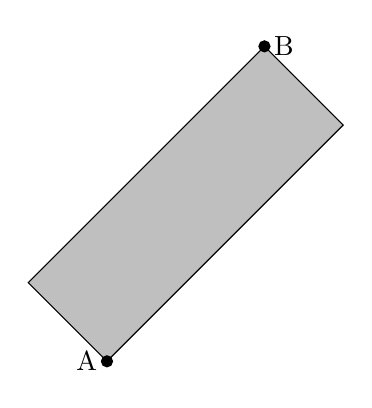
\begin{tikzpicture}
\fill [fill=lightgray] (0,0) -- (-1,1) -- (2,4) -- (3,3) -- cycle;
\draw  [latex-latex](0,0) -- (-1,1) -- (2,4)-- (3,3) -- cycle;

\filldraw (0,0) node[left] {A} circle (2pt);
\filldraw (2,4) node[right]{B} circle (2pt);
\end{tikzpicture}
\end{center}

Drop an altitude from B to line up horizontally with A and label the end-point D.
The length |AD| and |BD| are the coordinates.

\begin{center}
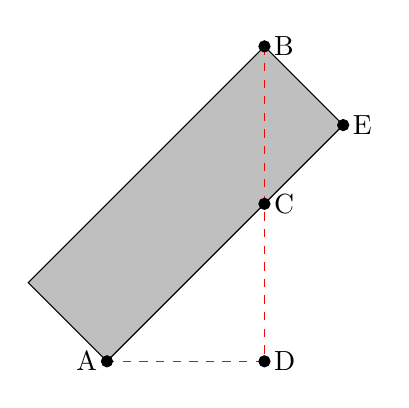
\begin{tikzpicture}
\fill [fill=lightgray] (0,0) -- (-1,1) -- (2,4) -- (3,3) -- cycle;
\draw  [latex-latex](0,0) -- (-1,1) -- (2,4)-- (3,3) -- cycle;

\draw[dashed,red] (2,4)-- (2,2)--(2,0) -- (0,0);

\filldraw (0,0) node[left] {A} circle (2pt);
\filldraw (2,4) node[right]{B} circle (2pt);
\filldraw (2,2) node[right]{C} circle (2pt);
\filldraw (2,0) node[right]{D} circle (2pt);
\filldraw (3,3) node[right]{E} circle (2pt);
\end{tikzpicture}
\end{center}

The triangles $\triangle$ACD and $\triangle$BCE are $45^\circ-90^\circ-45^\circ$ triangles meaning:
\begin{equation*}
\begin{aligned}
	\uline{AC} =& \sqrt{2}\uline{AD} \\
	\uline{BE} =& \frac{1}{\sqrt{2}}\uline{BC} \\
	=& \frac{1}{\sqrt{2}}(\uline{BD}-\uline{CD}) \\
	=& \frac{1}{\sqrt{2}}(\uline{BD}-\uline{AD}) \\
\end{aligned}
\end{equation*}

Hence the (signed) area of the rectangle is:
\begin{equation*}
\begin{aligned}
	\uline{BE}\cdot\uline{AE} =&\uline{BE}\cdot(\uline{AC}+\uline{CE}) \\
	=&(\uline{BD}-\uline{AD})(\uline{BD}+\uline{AD})\\
	=&\uline{BD}^2-\uline{AD}^2\\
\end{aligned}
\end{equation*}

\subsection{Causal Metric}
This construction supplies some intuition for Minkowski Metric.
Since if we interpret the plane as the set of events where the horizontal component is space-like and the vertical is time-like.
The reason the rectangle is at a $45^\circ$ is because that's the maximum speed of propagation.
The rectangle's area is a measure of the amount of events in-between the two.
And the sign of the area is the type of causal connection.
Wether the points are in the way (space-like), or another events are a means by which the earlier effect the later (time-like).

\let\uline\undefined

% Copyright 2023 Kieran W Harvie. All rights reserved.

\section{Integrals and Symmetry}

\subsection{Domain Symmetry} 
Let $U$ be a subset of $\mathbb{R}^n$ and let $\phi: U \rightarrow U$ be a function such that:
\begin{equation*}
\begin{aligned}
	\phi(U) &= U \\
	|\det\phi'(\mathbf{u})| &= 1 \\
\end{aligned}
\end{equation*}
Basically $\phi$ is a linear permutation\footnote{
	Note that $\phi$ being a permutation requires that if the magnitude of the determinate is constant it must be unity, this can be seen by setting $f$ to a constant.
}
on $U$, this is a symmetry in the most direct sense.
We obtain the following:
\\
\begin{equation*}
\begin{aligned}
	\int_{U}f(\mathbf{v})\,d\mathbf{v} =& \int_{\phi(U)}f(\mathbf{v})\,d\mathbf{v} \\
	=& \int_Uf(\phi(\mathbf{u}))|\det\phi'(\mathbf{u})|\,d\mathbf{u} \\
	=& \int_Uf(\phi(\mathbf{u}))\,d\mathbf{u} \\
\end{aligned}
\end{equation*}
\\

In particular we get:
\[0=\int_{U}\big(f(\mathbf{u})-f(\phi(\mathbf{u}))\big)\,d\mathbf{u}\]

This integral is important since a function can be split into a vanishing and non-vanishing part:
\begin{equation*}
\begin{aligned}
	f(\mathbf{u}) =& \frac{1}{2}\big(f(\mathbf{u})+f(\phi(\mathbf{u}))+\frac{1}{2}\big(f(\mathbf{u})-f(\phi(\mathbf{u}))\big) \\
	\int_Uf(\mathbf{u})\,d\mathbf{u} =& \frac{1}{2}\int_U\big(f(\mathbf{u})+f(\phi(\mathbf{u}))\,d\mathbf{u}+\frac{1}{2}\int_U\big(f(\mathbf{u})-f(\phi(\mathbf{u}))\big)\,d\mathbf{u} \\
	=& \frac{1}{2}\int_U\big(f(\mathbf{u})+f(\phi(\mathbf{u}))\,d\mathbf{u}\\
\end{aligned}
\end{equation*}
\\

For example, consider the classic odd function on an integral centered at $0$.
\[\phi(x) = -x \]
\[U = [-1,1]\]

We get the familiar:
\[\int_{-1}^{1}f(x)\,dx = \frac{1}{2}\int_{-1}^{1}\big(f(x)+f(-x)\big)\,dx\]
\\

The utility of this relation can be seen by applying it to the basis of a class of function.
Let $V = \langle 1,x,x^2 \rangle$, this is a basis for all parabolas.
Notice that $x$ base element vanishes, simplify the evaluation of integrals.
\\

For a 2-D example recall that for two dimensional change of variables:
\[ (x,y) = \phi(u,v) \]
We have:
\[|\det\phi'(\mathbf{v})| = \frac{\partial x}{\partial u}\frac{\partial y}{\partial v} - \frac{\partial x}{\partial v}\frac{\partial y}{\partial u} \]

The rotation symmetry for a regular triangle is:
\[(x,y) = \frac{1}{2}(-u-\sqrt{3}v,\sqrt{3}u-v)\]
\\

Obviously the symmetries act like a group and with functions being a vector space we can use group representations.

\subsection{Function Symmetry}
Let $f$ and $\phi$ be functions such that:
\[f(t) = \phi'(t)f(\phi(t))\]
Then for arbitrary $x_0$ and $x_1$ we have:
\begin{equation*}
\begin{aligned}
	\int^{x_1}_{x_0}f(t)\,dt =& \int^{\phi(x_1)}_{\phi(x_0)}\phi'(t)f(\phi(t))\,dt \\ 
	=& \int^{\phi(x_1)}_{\phi(x_0)}f(t)\,dt \\ 
	=& \int^{\phi(x_1)}_{x_1}f(t)\,dt+\int_{\phi(x_0)}^{x_1}f(t)\,dt \\ 
	\int^{\phi(x_0)}_{x_0}f(t)\,dt =& \int^{\phi(x_1)}_{x_1}f(t)\,dt \\ 
\end{aligned}
\end{equation*}
Hence the integral value is independent of $x_n$, in particular if $\phi$ has a fixed point then the integral is zero.

% Copyright 2023 Kieran W Harvie. All rights reserved.

\section{Discontinuities in a Non-decreasing Function}

Let $f$ be a non-decreasing function.

Define the jump function $J$ as:
\[ J(x) = \inf\{f(t) | t > x\} - \sup\{f(t) | t < x\}\]

This function is well defined since the sets are appropriately bound by $f(x)$. And it is clear that $J(d) \neq 0$ iff $d$  is a discontinuity and that $J$ is non-negative.
\\

Let $U = (x_0,x_1)$. For $d_n \in U$ with $n < m \Rightarrow d_n < d_m$ we have:
\[f(x_1)-f(x_0) \geq \sum_{k}J(d_k)\]

Proof:
\begin{equation*}
\begin{aligned}
	&\sum_{k}J(d_k) \\
	=& \inf\{f(t) | t > d_n\} - \sup\{f(t) | t < d_0\} + \sum_k\big[\inf\{f(t) | t > d_{k-1}\} - \sup\{f(t) | t < d_k\}\big] \\
	\leq & f(d_n)-f(d_0) + \sum_k\big[f(d_{k-1})-f(d_k)\big] \\
	\leq & f(d_n)-f(d_0)\\
	\leq & f(x_n)-f(x_0)\\
\end{aligned}
\end{equation*}

Let $ S_n = \{d \in U | J(d) > \frac{1}{n}(f(x_1)-f(x_0)) \}$
From the previous inequality there are at most $n$ elements in $S_n$.
Hence:
\[\{d\in U | J(d) > 0\} = \bigcup_{n}\left\{d \in U | J(d) > \frac{1}{n}(f(x_1)-f(x_0))\right\}\]
Is countable, hence the number of discontinuities of $f$ on $U$ is countable.
\\

By corollary the discontinuities of a non-decreasing function on $\mathbb{R}$ are countable:

Let $f$ be a non-decreasing function on $\mathbb{R}$.
Let $X_n = (n-1,n+1)$, clearly $\mathbb{R} = \bigcup_{n}X_n$\footnote{Having them overlap simplify the proof by avoiding literal edge-cases.}.
Assume $f$ has an uncountable number of discontinuities then at least one $X_n$ contains uncountable discontinuities.
Otherwise there would be a countable set of countable sets of discontinuities, making them countable.
But $f$ being non-decreasing function and having an uncountable number of discontinuities in $X_n$ is a contradiction.

% Copyright 2023 Kieran W Harvie. All rights reserved.

\section{Mean and Variance, and the arbitrariness thereof}
For some time I have wondered about the arbitrariness around the mean and variance.
For example why the arithmetic mean instead of the geometric or root-mean-squared?
And why square root the variance to give the standard deviation?

Well the strictness of Markov's and Chebyshev's might provide a reason.
Both rely of the conditional expected value, so just to reiterate:
\[E[X | X \geq a] \geq a \]
Since everything $X$ can be is greater then $a$ it's expected value must be greater than $a$. 
Notice the strictness of the inequality, this will be used to make the following inequalities much stricter.

\subsection*{Markov}
\begin{equation*}
\begin{aligned}
	\mu =& E[X]\\
	=& P(X \leq a)E[X|X \leq a] + P(X \geq a)E[X|X \geq a] \\ 
	\geq& 0\cdot E[X|X \leq a] + P(X \geq a)a \\ 
	\frac{\mu}{a}\geq& P(X \geq a) \\
\end{aligned}
\end{equation*}
% What if we move zero around?
% try Y = m X+c and see what happens.

\subsection*{Chebyshev}
\begin{equation*}
\begin{aligned}
	& E[(X-a)^2] \\
	=&P(|X-a| \leq b)E[(X-a)^2 | |X-a| \leq b] + P(|X-a| > b)E[(X-a)^2 | |X-a| > b]\\
\end{aligned}
\end{equation*}

\subsection*{A General Relation}
Assume:
\[f(S') \geq 0,\quad g(S) \geq 0\]
Then through:
\begin{equation*}
\begin{aligned}
	E[f(X)] =& P(X \in S)E[f(X) | X \in S] + P(X \in S' )E[f(X) | X \in S']\\
\end{aligned}
\end{equation*}
We have:
\begin{equation*}
\begin{aligned}
	1 - \frac{E[g(X)]}{E[g(X) | X \in S']} \leq P[X \in S] \leq \frac{E[f(X)]}{E[f(X) | X \in S]}\\
\end{aligned}
\end{equation*}
With dual equality if:
\[f = 1_S,\quad g = 1_{S'}\]

\subsection*{Covariance}
Lets try to find the lest squares regression between $X$ and $Y$ such that:
\[E[X] = E[Y] = 0, E[X^2] = E[Y^2] = 1\]
Since the expected values are both zero the line is through the origin
\begin{equation*}
\begin{aligned}
	\sum_{n}(mx_n+c-y_n)^2 =& nE[(mX+c-Y)^2] \\
	=& n \bigg(E[m^2X^2]+E[c^2]+E[Y^2]+E[2cmX]+E[-2mXY]+E[-2cY]\bigg)\\
	=& n(m^2+c^2+1-2mE[XY])\\
\end{aligned}
\end{equation*}
Trying to minimize this value by our selection of trivially gets:
\[c = 0,\quad m = E[XY]\]
Just expanding the definitions gives:
\[COV[X,Y] = E[(X-E[X])(Y-E[Y])] = E[XY] = m\]
Hence the covariance can `naturally' be interpreted and the first order function between the valuables.

\[E[f(X)] \approx E[f_0 + f_1X + f_2X^2/2] = f_0 + \mu f_1 + \sigma^2f_2/2\]
\[E[f(X)] \approx E[f(\mu) + (X-\mu)f'(\mu) + (X-\mu)^2/2f''(\mu)] = f(\mu) + \frac{f''(\mu)}{2}\sigma^2\]

% Consider a mention of Bessel's correction and the sum((x-(mu+a)^2) = sigma^2+a^2, general relation (square through AM-GM inequality)


\end{document}
